% !TeX encoding = UTF-8
\documentclass[bind,a4paper,table]{mythesis}

\usepackage{booktabs}
\usepackage{xcolor}
\usepackage{tabularx}
\usepackage{ltablex}
\usepackage{thesis}
%\usepackage[full,round]{harvard}%
\usepackage{natbib}%\bibpunct{(}{)}{;}{a}{,}{,}
\usepackage{pgfplots}
\usepackage{graphicx}
\usepackage{latexsym}
\usepackage{verbatim}
%\usepackage[latin1]{inputenc}
\usepackage[brazilian]{babel}
\usepackage[utf8]{inputenc}
\usepackage{amssymb}
\usepackage{amsmath}
\usepackage{amstext}
\usepackage{amscd}
\usepackage{amsthm}
\usepackage{fancyhdr,fancybox}
\usepackage{psfrag}
\usepackage{rotating}
\usepackage{url}
%\usepackage[colorlinks]{hyperref}
%\usepackage{listings}
\usepackage{epstopdf}
\usepackage{makeidx}
\usepackage{authorindex}
\usepackage{multirow}
\usepackage{picture}
\usepackage[algochapter,algoruled,linesnumbered,lined,portuguese]{algorithm2e}
%\usepackage{algorithmic2e}
%\usepackage[ruled,vlined,portuguese]{algorithm2e}
%\usepackage{algorithm}
%\usepackage{algorithmic}
%\usepackage[noend]{algpseudocode}
%\usepackage{rotating}
\usepackage{tocbibind}
\usepackage{array}
\usepackage{lscape}
\usepackage{caption}
%\usepackage{ragged2e}

\usepackage{rotating}
\usepackage{longtable}
\usepackage{listings}
\usepackage{graphicx}
\usepackage{url}
\usepackage{cancel}
\usepackage{scalefnt}
\usepackage{makecell}
\usepackage{todonotes}
\usepackage{wrapfig}

\usepackage{float}
\restylefloat{figure}
\newcommand{\specialcell}[2][c]{\begin{tabular}[#1]{@{}c@{}}#2\end{tabular}}

\usepackage{pifont}% http://ctan.org/pkg/pifont
\newcommand{\cmark}{\ding{51}}%
\newcommand{\xmark}{\ding{55}}%


%\input{tex/defs.tex}
\makeindex

\newcommand{\listofalgorithmes}{\tocfile{\listalgorithmcfname}{loa}}

\newcommand{\hardware }{\textit{hardware}}
\newcommand{\Hardware }{\textit{Hardware}}
\newcommand{\software }{\textit{software}}
\newcommand{\Software }{\textit{Software}}
\newcommand{\hardwares}{\textit{hardwares}}
\newcommand{\Hardwares}{\textit{Hardwares}}
\newcommand{\softwares}{\textit{softwares}}
\newcommand{\Softwares}{\textit{Softwares}}

\newcommand{\hs}{\textit{hardware}\ e\ \textit{software}}
\newcommand{\HS}{\textit{Hardware}\ e\ \textit{Software}}

\newcommand{\wearable} {\textit{wearable}}
\newcommand{\Wearable} {\textit{Wearable}}
\newcommand{\wearables}{\textit{wearables}}
\newcommand{\Wearables}{\textit{Wearables}}


\newcommand{\design}   {\textit{design}}
\newcommand{\designer} {\textit{designer}}
\newcommand{\Design}   {\textit{Design}}
\newcommand{\Designer} {\textit{Designer}}
\newcommand{\designs}  {\textit{designs}}
\newcommand{\designers}{\textit{designsers}}
\newcommand{\Designs}  {\textit{Designs}}
\newcommand{\Designers}{\textit{Designers}}
\newcommand{\assembly} {\textit{assembly}}
\newcommand{\profile}  {\textit{profile}}
\newcommand{\Profile}  {\textit{Profile}}
\newcommand{\speedup}  {\textit{speedup}}
\newcommand{\Speedup}  {\textit{Speedup}}
\newcommand{\core}     {\textit{core}}
\newcommand{\cores}    {\textit{cores}}
\newcommand{\codesign} {\textit{codesign}}
\newcommand{\mobile}   {\textit{mobile}}
\newcommand{\benchmark}   {\textit{benchmark}}
\newcommand{\benchmarks}   {\textit{benchmarks}}
\newcommand{\Benchmark}   {\textit{Benchmark}}
\newcommand{\Benchmarks}   {\textit{Benchmarks}}
\newcommand{\titulo}{Uma Abordagem do Problema de Particionamento \Hardware\ e \Software\ para \Design\ de Sistemas Computacionais \Wearables}

\newcommand{\A}{$\mathcal{A}$}
\newcommand{\B}{$\mathcal{B}$}
\newcommand{\C}{$\mathcal{C}$}

\newenvironment{VarDescription}[1]%
  {\begin{list}{}{\renewcommand{\makelabel}[1]{\hspace{0cm}\hfil\textbf{##1}  :}%
    \settowidth{\labelwidth}{\hspace{0cm}\textbf{#1} :}%
    \setlength{\leftmargin}{\labelwidth}\addtolength{\leftmargin}{\labelsep}}}%
  {\end{list}}

\newcounter{matriz}
\newenvironment{matriz}{\refstepcounter{matriz}\equation}{\tag{M\thematriz}\endequation}


%\input{macros}

%% PDF metadata
\makeatletter
\@ifpackageloaded{hyperref}{%
  \hypersetup{%
  colorlinks=false,
  pdftitle = {Uma Abordagem do Problema do Particionamento \Hardware\ e \Software\ para \Design\ de Sistemas Computacionais \Wearables},
  pdfsubject = {Rodolfo Labiapari Mansur Guimarães's MsC thesis},
  pdfkeywords = {Wearable, FPGA, Hardware Software Partitioning},
  pdfauthor = {\textcopyright\ Rodolfo Labiapari Mansur Guimarães}}
}{}
\makeatother

%Hyphenations
\hyphenation{XHSTT}
%\hyphenation{res-tri-ções}
\hyphenation{co-nhe-ci-do}
\hyphenation{co-nhe-ci-da}
\hyphenation{re-a-li-za}
\hyphenation{vi-zi-nho}
\hyphenation{clim-bing}
\hyphenation{ran-king}
\hyphenation{me-lhor}
\hyphenation{ou-tras}
\hyphenation{ge-ra-das}
\hyphenation{ex-pe-ri-men-tos}
\hyphenation{pro-ble-ma}
%\hyphenation{su-ges-tões}
\hyphenation{pos-te-rior-men-te}


%% Define the thesis title and author
\begin{document}
\let\cleardoublepage\clearpage
\title{\titulo}
\author{Rodolfo Labiapari Mansur Guimarães}%% Start the document

%% Define the un-numbered front matter (cover pages, rubrik and table of contents)
\begin{frontmatter}
	\selectlanguage{brazilian}
	% !TeX spellcheck = pt_BR
%!TEX root = ../main_text.tex
\let\cleardoublepage\clearpage
\titlepage[Universidade Federal de Ouro Preto]{

\vspace{-21cm}
\textbf{UNIVERSIDADE FEDERAL DE OURO PRETO}

\vspace{13cm}

Orientador: Dr. Ricardo Augusto Rabelo Oliveira \\ \vskip8pt

\vspace{3cm}

\hspace{7.5cm}
\parbox{0.5\textwidth}{
Dissertação submetida ao Instituto
de Ciências Exatas e Biológicas da Universidade
Federal de Ouro Preto para qualificação ao
título de Mestre em Ciência da Computação
}

\vspace{2.8cm}

\begin{center}
Ouro Preto, Setembro de 2018 \todo{alterar}
\end{center}
}

\let\cleardoublepage\clearpage

\titlepage[Universidade Federal de Ouro Preto]{
\vspace{-21cm}
\textbf{}
\vspace{13cm}

Orientador: Dr. Ricardo Augusto Rabelo Oliveira \\ \vskip8pt

\vspace{3cm}

\begin{figure}[h!]
  \begin{center}
    
\includegraphics[width=1.0\textwidth]{img/logo.png}
    \label{fig:goal}
  \end{center}
\end{figure}

}

%\begin{figure}[h]
 % \begin{center}
  %  \includegraphics[width=1.0\textwidth]{img/ataDefesa.pdf}
   % \label{fig:ataDefesa}
  %\end{center}
%\end{figure}

\begin{comment}

\dedication{\vspace{4cm}
\begin{flushright}
Dedico este trabalho a você que sempre me fez acreditar na realização dos meus sonhos e trabalhou muito para que eu pudesse realizá-los, \emph{Mãe}. A minha \emph{família} e \emph{amigos} que sempre me apoiaram nas horas difíceis. Ao meu \emph{pai}, que mesmo distante influenciou para que pudesse chegar até aqui.

\end{flushright}

}
\end{comment}

%% Abstract in portuguese
\begin{abstract}[\smaller \titulo\\ \vspace*{1cm} \smaller Resumo]
  %\thispagestyle{empty}
%1) Contextualização: É a parte que está lá, onde vc passa a ideia geral da área.
%2) Gap: O que ainda falta na área que foi contextualizada? (especificamente o problema no qual vc "toca").
%3) Propósito: O que o seu artigo faz? Que tipo de problema vc está endereçando?
%4) Metodologia: O que vc utilizou no desenvolvimento do seu artigo.
%5) Resultados: Qual foi o principal (ou os principais resultados) obtidos?
%6) Conclusões: Qual a sua conclusão mais relevante?


%1) Contextualização: É a parte que está lá, onde vc passa a ideia geral da área.
As tecnologias em microeletrônica, sensores e comunicação móvel têm sido constantemente melhoradas à medida que a informação torna-se mais necessária. 
Tornam-se um estímulo para o desenvolvimento de sistemas computacionais inteligentes e conectados como sistemas embarcados, IoTs ou \wearables,\ visto pelo rápido desenvolvimento desses para o mercado.
Tais dispositivos utilizam vários sensores e necessitam de um serviço autônomo, o que implica numa grande demanda de desempenho somado com o baixo consumo de energia. 
Entretanto ainda com a dificuldade de satisfazer os requisitos de aumento de desempenho e redução de consumo energético das várias aplicações autônomas modernas.
%Utilizam de um conjunto de sensores e necessitam de um serviço autônomo, o que implica numa demanda de desempenho somado com o baixo consumo de energia.
%
%2) Gap: O que ainda falta na área que foi contextualizada? (especificamente o problema no qual vc "toca").
Análise de desempenho no uso de FPGA com particionamento em \hardware\ para sistemas embarcados têm sido fortemente abordada pela comunidade acadêmica. 
Entretanto, não há trabalhos científicos que trabalham o particionamento para sistemas \wearable.
%
%3) Propósito: O que o seu artigo faz? Que tipo de problema vc está endereçando?
Esta pesquisa tem como objetivo o aprimoramento de desempenho de dispositivos computacionais \wearables\ em \hardwares\ reconfiguráveis, visando alocação de recursos em \hardware\ e reduzindo o consumo energético%
%
%4) Metodologia: O que vc utilizou no desenvolvimento do seu artigo. Deve ser curto.
, isso utilizando particionamento \hs\ como meio.
%
%5) Resultados: Qual foi o principal (ou os principais resultados) obtidos? 
%6) Conclusões: Qual a sua conclusão mais relevante?
Os resultados mostram que é possível obter maior desempenho em sistemas \wearables\ utilizando plataforma FPGA apenas com a realocação de algoritmos candidatos em \hardware.


Palavras-chave: Particionamento \hs, Sistema \Wearable, FPGA, Performance.



\begin{comment}
Este trabalho constitui-se de uma abordagem do problema de particionamento \hs\ para dispositivos vestíveis com foco em aumento de performance, visando o gasto de recursos em seu \textit{trade-off}.
A tecnologia digital de fatores como microeletrônica, sensores e comunicação móvel são constantemente melhoradas à medida que a informação torna-se cada vez mais sem-fio, tornando-a um grande estímulo para o desenvolvimento de dispositivos inteligentes e conectados como sistemas embarcados IoT ou vestíveis (do inglês \wearables). 
Isso é visto no rápido desenvolvimento de dispositivos para comércio, entretanto, ainda com a dificuldade de satisfazer os requerimentos das várias aplicações modernas. 
Tais dispositivos utilizam de um leque enorme de sensores e necessitam de um serviço autônomo, o que implica numa grande demanda de performance somado com o baixo consumo de energia sem deixar design, segurança e confiabilidade a desejar. 
Para obter um produto de alta qualidade, atendendo aos requisitos solicitados, esta pesquisa consiste na análise de projetos para sistemas \wearables\ utilizando plataformas FPGA como meio na realização de particionamentos \hs\ obtendo um bom \speedup\ e eficiência em comparação a outros sistemas como \textit{in-software}. 
%Com mais pesquisas voltadas para saúde e conforto humano, os dispositivos \wearables\ estão possuindo cada vez mais habilidades para detectar e identificar pessoas ou seus comportamentos e assim tornar um complemento/auxílio para as atividades cotidianas.

%To adequately address these demands, sophisticated embedded computing and embedded design technologies are needed. After an introduction to modern mobile systems, this paper discusses the huge heterogeneous area of these systems, and considers serious issues and challenges in their design. Subsequently, it discusses the embedded computing and design technologies needed to adequately address the issues and overcome the challenges in order to satisfy the stringent requirements of the modern mobile systems.
Palavras-chave: Particionamento \hs, Sistema \Wearable, Sistemas Embarcados.
\end{comment}
\end{abstract}
\let\cleardoublepage\clearpage


%% Abstract
\begin{abstract}[\smaller An Approach of Hardware and Software Partitioning for the Design of Wearable in Reconfigurable Hardware\\ \vspace*{1cm} \smaller Abstract]

  %\thispagestyle{empty}
 
This work consists of an approach \todo[inline]{a}of the hardware and software partitioning problem for wearable devices focused on performance enhancement, aiming at the expense of resources in their trade-off.
The digital technology of factors such as microelectronics, sensors and mobile communication are constantly improved as information becomes increasingly wireless, making it a great stimulus for the development of intelligent and connected devices like embedded IoT or wearable systems.
This is seen in the rapid development of devices for commerce, however, still with the difficulty of satisfying the requirements of the various modern applications.
Such devices use a wide range of sensors and require autonomous service, which implies a great demand for performance coupled with low power consumption without leaving design, security and reliability to be desired.
In order to obtain a high-quality product, meeting the requested requirements, this research consists of the analysis of designs for wearables systems using FPGA platforms as a means of realizing hardware and software partitions obtaining good speedup and efficiency compared to other systems such as in-software.

Keywords: Hardware and Software Partitioning, Wearable System, Embedded System.
\end{abstract}


\let\cleardoublepage\clearpage
%% Declaration
\begin{declaration}
Esta dissertação é resultado de minha própria pesquisa, exceto onde referência explícita é feita ao trabalho de outros, e não foi submetida para outra qualificação nesta nem em outra universidade.
\vspace*{1cm}
\begin{flushright}
Rodolfo Labiapari Mansur Guimarães
\end{flushright}
\end{declaration}

\begin{comment}
%% Acknowledgements
\let\cleardoublepage\clearpage
\begin{acknowledgements}

Primeiramente agradeço à Deus por me amparar nos momentos difíceis e me dar força para superar as dificuldades.

Aos meus pais, Hudson e Márcia Inês, à minha irmã Rúbia e minha namorada Olívia, pelo incentivo, apoio e afeto.

À minha madrinha Lucianara, por sempre acreditar nos meus sonhos.

À toda minha família, pelo carinho e força.

Agradeço ao meu orientador Ricardo Augusto Rabelo Oliveira pela oportunidade concedida, orientação e apoio no desenvolvimento do trabalho. 

Aos meus amigos do laboratório iMobilis Breno Keller, Mateus Coelho, Maurício Silva, Michael Pacheco, Rafael Ferreira, Renato Vilarinho, Ricardo Câmara, Thiago D'Angelo e Vicente Amorim pela ajuda, pelas longas horas de trabalho, amizade, carinho e força, fundamentais para que eu conseguisse chegar até aqui.

À República Dominakana, moradores e ex-alunos, por me acolherem, pelo companheirismo e amizade, tornando esta minha segunda casa.

Ao CNPq, à FAPEMIG, à CAPES e à UFOP pelo apoio recebido no desenvolvimento deste trabalho.

Ao PPGCC/UFOP, professores e técnicos pela ajuda sempre que fez-se necessário.

Enfim, agradeço a todos que, de alguma forma, acreditaram e torceram por mim, participaram de minha vida e ajudaram na realização deste trabalho.

\end{acknowledgements}
\end{comment}


%% Preface
%\begin{preface}
%
%\end{preface}

% ToC
\tableofcontents
\listoffigures
\let\cleardoublepage\clearpage
\listoftables
%%\listofalgorithms
\listofalgorithmes

\begin{comment}

%% Strictly optional!
\frontquote%
{Talvez não tenha conseguido fazer o melhor, mas lutei para que o melhor fosse feito. Não sou o que deveria ser, mas Graças a Deus, não sou o que era antes.}%
{Marthin Luther King}

\end{comment}

\end{frontmatter}

%% Start the content body of the thesis
\begin{mainmatter}
  \selectlanguage{brazilian}
  	%!TEX root = ../main_text.tex

\chapter*{Nomenclaturas}
\addcontentsline{toc}{chapter}{Nomenclatura}
\markboth{Nomenclaturas}{Nomenclaturas}

%% Nomenclature
\begin{tabular*}{20cm}{lp{12cm}}
ASIC  & \textit{Application-Specific Integrated Circuit} \\
CI    & \textit{Circuito Integrado} \\
CUDA  & \textit{Compute Unified Device Architecture} \\
CPU   & \textit{Central Processing Unit} \\
CSoC  & \textit{Configurable System on a Chip} \\
DRES  & \textit{Dynamically Reconfigurable Embedded Systems} \\
FPGA  & \textit{Field-Programmable Gate Array} \\
FPLD  & \textit{Field-Programmable Logic Device} \\
GA    & \textit{Genetic Algorithm} \\
GC    & \textit{Grafo de Chamada} \\
GFC   & \textit{Grafo de Fluxo de Controle} \\
GPU   & \textit{Graphical Processing Unit} \\
HDL   & \textit{Hardware Description Language} \\
HLS   & \textit{High-Level Synthesis} \\ 
IoT   & \textit{Internet of Things} \\
LED   & \textit{Light-Emitting Diode} \\
LUT   & \textit{Look-Up Table} \\
NRE   & \textit{Nonrecurring Engineering} \\
PLD   & \textit{Programmable-Logic Device} \\
RAM   & \textit{Random-Access Memory} \\
\end{tabular*}

\begin{tabular*}{20cm}{lp{12cm}}
   SRAM  & \textit{Static Random-Access Memory} \\
   VGA   & \textit{Video Graphics Array} \\
   VHDL  & \textit{VHSIC Hardware Description Language} \\
   VHSIC & \textit{Very High Speed Integrated Circuits} \\
\end{tabular*}

%se tiver mais de uma página usar outra tabela
%\begin{tabular*}{20cm}{lp{12cm}}
%$\emph{fem}$ & Força eletromotriz\\
%\end{tabular*}

	\let\cleardoublepage\clearpage
	% !TEX root = ../main_text.tex
% !TeX encoding = UTF-8
\chapter{Introdução} \label{chap:introducao}

   %\todo[inline]{contextualização lógica}
	%intro geralzona
	O recente progresso na obtenção e manipulação de informações, em conjunto com a ascensão da tecnologia da microeletrônica, comunicação e sensores, proporcionou um enorme estímulo no desenvolvimento de sistemas computacionais inteligentes de comunicação e \wearables, todos sendo dispositivos embarcados \citep{Jozwiak2017}.
	%
	O projeto de sistemas computacionais está mais complexo que nunca. A demanda por curto tempo para disponibilidade ao mercado, somado ao fato dos produtos exigirem propriedades de corretude, rapidez, confiabilidade e preço acessível, representam um desafio para projetistas de sistemas embarcados em geral.
	Sistemas computacionais embarcados (também nomeados pela literatura como sistemas embarcados ou sistemas embutidos) possuem muitos componentes implementados tanto em \hs\ e esta decisão de escolha de local de implementação será o tema principal abordado neste documento com foco em dispositivos \wearable.

	% embedded 
   %\todo[inline]{A parte de wearable vc tem q explorar mais no capitulo 1 tb, como construcao da motivacao. Uma introducao tem q ser a sequinte sequencia}
	Os sistemas computacionais embutidos são produtos que utilizam processadores ou controladores e podem estar desde fornos de microondas, até sistemas de controle de aeronaves.
   São computadores situados em dispositivos e que sua presença não é imediatamente óbvia.
	Requerem técnicas na qual difere das utilizadas para \design\ de computadores de propósito geral ou aplicações de \software\ dessas máquinas \citep{Wolf1994}.  
	Em 2015, foi previsto um total de 6,5 bilhões de dispositivos ativamente conectados para o ano de 2016, segundo notícias da empresa de pesquisa e consultoria Gartner \citep{RobvanderMeulen2015}.
	
	% wearable
	No âmbito de sistemas embutidos, existe um subconjunto na qual possui o propósito de integrar-se ao sistema corporal expandindo suas capacidades. 
	Esses dispositivos `vestíveis', chamados de sistemas \wearables, envolvem grande volume de dados de múltiplos sensores ou outros sistemas e são requeridos para prover serviço autônomo, contínuo, em um longo período de tempo.
   Diferentemente de \textit{smartphones} e \textit{tablets}, os \wearables\ são tecnologias eletrônicas ou computadores que são incorporados ao vestuário dos usuários criando uma integração cada vez mais intensa entre tecnologia e ser humano. 
   Sua tendência é superar os dispositivos manuais como computadores e telefones pois são dispositivos mais sofisticados pela existência de recursos sensoreais e escaneamento.
   %
   Cerca de 20\% da população possui pelo menos um dispositivo sendo que 10\% utiliza-o todos os dias \citep{lee2016information}.
   São dispositivos que permitem benefícios como um estilo de vida inspirado em dados \textit{fitness} até realidade aumentada preenchida por objetos virtuais.
	Tais dispositivos demandam de uma alta performance e/ou baixo consumo de energia, sem apresentar \textit{trade-off} de confiabilidade e segurança entre outros. % \citep{Jozwiak2017}.
	%
	Segundo o trabalho de \citet{Jozwiak2017}, com computação de alta performance e estudos em gasto energético eficiente, foi possível a facilitação do rápido progresso da computação móvel e autônoma.
	%Tudo isso deve-se à possibilidade de comunicar-se com a rede global de comunicação, combinada com o progresso de sensores e atuadores, criando novas oportunidades importantes de projeto.
	%%Exemplos disso são indústrias inteligentes, cidades e casas, bem como setores de IoT, sistemas móveis como automóveis inteligentes, computação móvel como \textit{smartphones}, comunicação e, não menos importante, os sistemas computacionais \wearable.
	Sistemas computacionais \wearables\ podem ser definidos como `embutidos que foram inseridos em ambiente \mobile\ de seus usuários, não exercendo a mesma atividade' e seu propósito é criar dispositivos com acesso constante, conveniente, portátil e principalmente \textit{hands-free}, aplicando não só na área de saúde e esportiva, mas também em entretenimento e assim por diante.

   %\todo[inline]{1- Apresnetar o problema:}
   \section{Problema}
	% intro particionamento
	A redução do ciclo de comercialização de um produto e o aumento de sua eficiência de desenvolvimento de projeto tem se tornado uma preocupação na área de \design\ de sistemas embarcados, incluindo também os \wearables.
	E por este motivo, a técnica de particionamento \hs\ tem sido uma das principais tecnologias para o desenvolvimento de sistemas embarcados em geral, desde que, este afeta a performance do sistema como um todo. 
   Para \citet{Hassine2017}, uma das soluções mais elegantes na computação que provê otimizações sistêmicas sobre essas circunstâncias é por meio do particionamento \hs.
	Segundo \citet{Wolf1994}, sistemas embutidos gerais são considerados únicos pelo fato da necessidade de um \codesign\ de \hs. 
   As pesquisas em \codesign\ de \hs\ têm como objetivo o \design\ de sistemas heterogêneos, visando performance, custo e metas de confiabilidade \citet{Edwards1994}.
	
   \begin{comment}
   
   Um exemplo simbólico de \codesign\ para o particionamento pode ser ilustrado na Figura \ref{fig:rt-edwards_partitioning} no qual um módulo em \software\ é substituído por um componente em \hardware\ executando a mesma tarefa mas com maior performance.
   
   \begin{figure}[h] \centering
   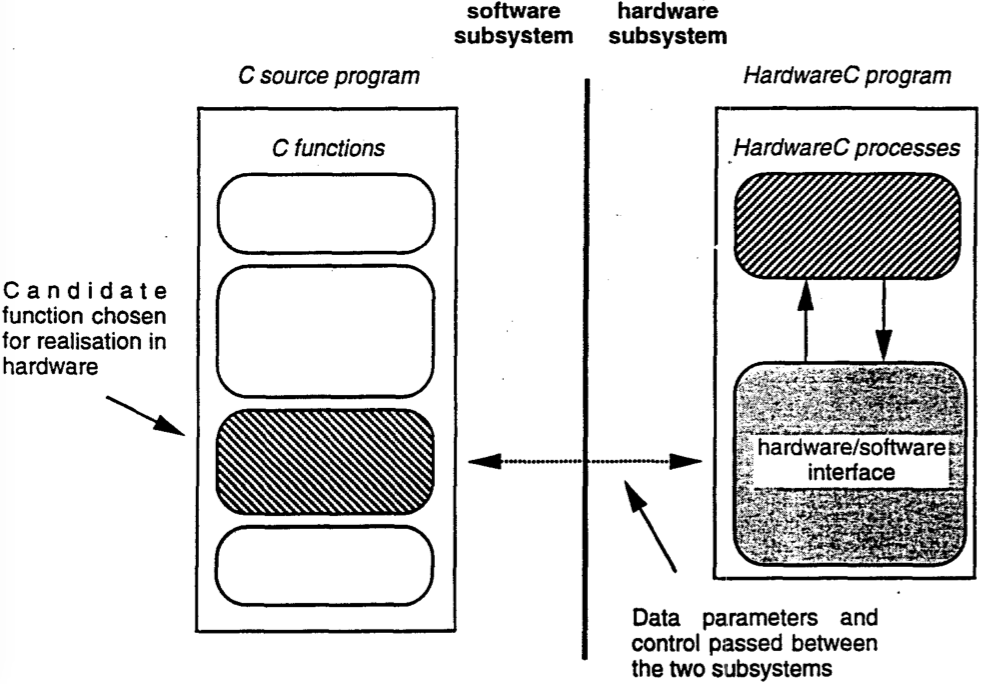
\includegraphics[width=0.7\textwidth]{img/rt-edwards_partitioning.png}
   \caption{Ilustração de um particionamento no \codesign\ de um sistema embarcado. Fonte: \citet{Edwards1994}.}
   \label{fig:rt-edwards_partitioning}
   \end{figure}
\end{comment}

	\citet{Hidalgo1997} dizem que o objetivo principal é o balanceamento de todas as tarefas de forma a otimizar alguns objetivos de sistema sobre determinadas restrições.
	Agrupar específicos conjuntos de instruções de uma aplicação e então mapear esses grupos tanto em \hs.
	%Os grupos designados ao \software\ são executados sequencialmente pelo respectivo processador do sistema enquanto os mapeados em \hardware\ são implementados por uma combinação customizada ou por circuitos sequenciais \citep{Sass2010}.

	% particionamento
	%Quando necessita de performance ao realizar o \codesign\ (termo referente ao inglês \textit{Participatory Design}) de \hs\ para sistemas embutidos, o problema de qual função do sistema deverá ser implementada em \hardware\ ou em \software\ emerge e esse problema é conhecido por particionamento \hs\ (\textit{hardware/software partitioning}).
	%Um significante esforço foi posto nesta área nos últimos dez anos, segundo \citet{Trindade2016}.
   
   Um desafio de \design\ é combinar a flexibilidade de demanda pelos vários ambientes e aplicações, e a alta performance exigida em tarefas com o baixo consumo de energia requerido para maximizar o tempo de uso da bateria.

   %\todo[inline]{3- Motivacao pra resolver este problema:}

	%Com o desenvolvimento de sistemas embutidos cada vez mais complexos, o particionamento \hs\ tornou-se um problema de otimização em \codesign\ de sistemas \citep{Yan2017}. 
   A motivação é que, tal problema que envolve \design\ colaborativo e multidisciplinar, é um passo-chave no \design\ de produtos modernos \citep{Trappey2016}. 
   Implementações que baseiam-se somente em módulos de \software\ possuem mais flexibilidade e menos custosos, entretanto, seu custo eleva-se em termos de tempo de execução. Uma implementação de \hardware\ customizada de um conjunto de computações proverá uma eficiência energética e \speedup\ maior relativa à implementações em \software\ \citep{Zhang2008, Hassine2017, Wolf1994, Canis2011, Stone2010}.

   % combinação de fpga com cpu
   A tendência hoje para \design\ é na combinação das funções do processador com os recursos dos arranjo de portas programáveis em campo (FPGAs, do inglês \textit{Field-Programmable Gates Array}) formando um sistema computacional híbrido. %, exemplo exibido na Figura \ref{fig:i-soc}. %\citep{Plessl2003}
   %O conceito de CSoC é importante quando necessita da construção de sistemas computacionais que podem utilizar de circuitos junto à um processador como é o caso de sistemas embutidos.
	Ao utilizar do FPGA para o problema de particionamento, é possível acelerar uma aplicação usando recursos de \hardware\ melhorando no desempenho e eficiência energética em comparação com o \software\ executado inteiramente em um processador \citep{Cong2009, Lo2009, Zhang2008a}. 
   %A Microsoft em \citeyear{Putnam2014} aceleraram o \textit{Bing Search} em duas vezes com a utilização de FPGAs em seus \textit{data centers} \citep{Putnam2014}.
   %além da aquisição da Altera, uma das duas maiores vendedoras de FPGAS no mundo, pela Intel em \citeyear{Maan2015} por cerca de $ 16.7 $ bilhões de dólares \citep{Maan2015}.


   %{4- Contribuicao ao resolver o problema:}

   %{5- Objetivos:}
   
   Este trabalho então, propõe o estudo e aplicação de técnicas de particionamento dentro do conjunto de aplicações e sistemas \wearable, na qual, possui restrições significativas como bateria, recursos e custo.

\section{Objetivos da Dissertação}
	Este trabalho tem como objetivo a abordagem do particionamento \hs\ bem como sua importância no mundo de sistemas computacionais embutidos, com foco em sistemas \wearables\ apresentando algumas soluções utilizadas atualmente.

    \begin{itemize}
      %\item Apresentação do tema de projeto de sistemas computacionais \wearable\ por meio do particionamento \hs;
      %\item Apresentação de uma abordagem metodológica criada para o uso ao problema aplicado no contexto desses sistemas \wearable, na qual possuem restrições relacionados ao custo energético e recursos.
      
         \item Introdução de sistemas computacionais \wearables\ e apresentação do problema de particionamento \hs\ no âmbito de de sistemas computacionais embutidos, com foco em sistemas \wearables;
         
         \item Apresentação das principais soluções apresentadas ao logo dos anos e as utilizadas atualmente, bem como as ferramentas HLS como LegUp e OpenCL para a geração de sistemas computacionais que usufruem de aceleradores em \hardware.
         
         \item Exposição da abordagem metodológica a ser utilizada para a procura da solução do problema de particionamento \hs\ apresentado.
    \end{itemize}

   \subsection{Justificativa}

   %{2- Justificativa pq eh um problema relevante:}
	A justificativa para a realização deste é que, além do tema de particionamento ser proposto recentemente, com o desenvolvimento de \designs\ mais complexos, esse problema de decisão torna-se cada vez mais desafiador para os \designers\ de projeto, no qual o grande requisito para eficiência necessariamente segue junto com a alta velocidade de processamento \citep{Trindade2016, Arato2005, Yan2017}.
	
	Dessa forma, pesquisá-lo com foco em sistemas \wearable\ torna-o ainda mais necessário pela pouca atenção dada pelo meio científico até o presente momento, como será demonstrado no decorrer do documento, principalmente pelo ampla utilização que este tipo de produto vem ganhando no espaço comercial.


   \subsection{Contribuição}
    
      O trabalho consiste numa busca sobre o aprimoramento de performance de um dispositivo computacional \wearable\ visando os respectivos gastos relativos ao uso de aceleradores em \hardware\ como recursos, gasto energético, área utilizada e outros itens que serão discutidos neste documento. 
       

\section{Organização da Dissertação}
	Os demais capítulos deste trabalho estão organizados da seguinte forma: 
   No Capítulo \ref{chap:revisao_bibliografica} é apresentada uma revisão bibliográfica do problema, abordando alguns métodos de fundamental importância para este trabalho. 
   No Capítulo \ref{chap:relacionados} são descritos alguns trabalhos relacionados ao tema abordado. 
   Nos Capítulos \ref{chap:design} e \ref{chap:met2} são apresentadas as metodologias, sendo a primeira a exibição do processo de \design\ e a segunda a metodologia proposta. 
   %No Capítulo \ref{chap:experimentos} \todo{são?} apresentados os resultados e suas considerações para o problema. 
   No Capítulo \ref{chap:conclusao} são apresentadas as conclusões parciais e propostas de trabalhos futuros.
	% !TeX spellcheck = pt_BR
% !TEX root = ../main_text.tex
% !TeX encoding = UTF-8
\chapter{Introdução} \label{chap:introducao}
    \todo[inline]{procurar por '?'}
    \todo[inline]{wearables sistemas wearables} % to querendo tudo para ou sistemas ou computação ou dispositivo wearable
    \todo[inline]{SEs}
    
    
    %\todo[inline]{1) Contextualização: Apresente uma visão da área identificando a importância do contexto q está trabalhando. Introduza os "termos" mais importantes.}
    
    %O projeto de Sistemas Embarcados (SE) está cada dia mais complexo \citep{Jozwiak2017}. 
    %
    O recente progresso na obtenção e manipulação de informação, em conjunto com a ascensão das tecnologias microeletrônica, comunicação e sensores proporcionaram um enorme estímulo no desenvolvimento de sistemas computacionais embarcados \citep{Jozwiak2017}.
    %
    A demanda por curto tempo para disponibilidade de produtos ao mercado somado em exigirem propriedades como alto desempenho, baixo consumo de energia e alocação de recursos, representam um desafio para projetistas de sistemas.% \wearables.
    
    % wearable
    Sistemas \Wearables,\ subcategoria de Sistemas Embarcados (SE), possuem o propósito de integrarem-se ao sistema corporal, expandindo suas capacidades e criando uma integração cada vez mais intensa entre ser humano e tecnologia, sendo sua presença não imediatamente óbvia.
    Envolvem múltiplos sensores ou outros sistemas e são requeridos para prover serviço autônomo, contínuo, em um longo período de tempo.
    
    Esses sistemas possuem diversos componentes implementados em \hs\ e ainda é um desafio combinar alto desempenho com baixo consumo de energia maximizando o tempo de uso \citep{Wolf1994, Edwards1994}.
    %
    Uma das maneiras de lidar com tais problemas consiste na combinação das funções do processador/controlador com os recursos dos Arranjo de Portas Programáveis em Campo (FPGAs, do inglês \textit{Field-Programmable Gates Array}) formando um sistema computacional híbrido.
    
    
    %particionamento
    A decisão tomada na escolha de nível de implementação de cada seção de código nesses sistemas é chamada de Particionamento \HS\ (também abreviado como particionamento). 
    Trata-se da escolha onde cada seção de código será implementada sendo ela em nível de \software\ por meio de execução pelos controladores ou em \hardware\ por meio de circuitos digitais dedicados à função e tem-se mostrado promissora aumentando o desempenho destes sistemas \citep{Sass2010, BenHajHassine2017}.
    %
    As pesquisas em \codesign\ de \hs\ têm como objetivo o \design\ de sistemas heterogêneos, visando desempenho, custo e metas de confiabilidade \citep{Edwards1994}.
    
    
    
    
    
    %\todo[inline]{3) Descreva o estado da arte atual, sempre referenciando trabalhos importantes.}
    
    Trabalhos como de \citet{Zhang2008, BenHajHassine2017, Wolf1994, Stone2010} mostram que, uma implementação customizada em \hardware\ pode prover maior eficiência energética e \speedup,\ sendo este a comparação de desempenho à implementações em \software.\ 
    %
    %\todo[inline]{2) Gap: Quais são as questões em aberto, restrições e limitações do estado atual dessa pesquisa.}
    %
    Entretanto, mesmo com vários estudos relacionados à desempenho com particionamento de SE em plataformas FPGA, não há estudos que avaliam a melhoria de desempenho especificamente para \wearables\ em plataformas FPGA.
    
    A motivação é que tal problema que envolve \design\ colaborativo e multidisciplinar, é um passo-chave no \design\ de produtos modernos \citep{Trappey2016}. 
    Com o desenvolvimento de \designs\ mais complexos, esse problema torna-se cada vez mais necessário, no qual o grande requisito para eficiência necessariamente segue junto com a alta velocidade de processamento \citep{Trindade2016, Arato2005, Yan2017}.
    Implementações que baseiam-se somente em módulos em nível de \software\ possuem mais flexibilidade e são menos custosos, entretanto, seu custo eleva-se em termos de tempo de execução. 
    Uma implementação de \hardware\ customizada de um conjunto de instruções proverá uma eficiência energética e \speedup\ maior relativa à implementações em \software\ \citep{Zhang2008, BenHajHassine2017, Wolf1994, Stone2010}.
    
    
    
    %\todo[inline]{4) Propósito+metodologia: Descreva o propósito do seu artigo utilizando para isso uma pitada da sua metodologia.}
    
    Dessa forma, esta pesquisa consiste no particionamento de alguns algoritmos candidatos do \wearable\ comparando o desempenho, alocação de recursos e gasto energético de ambas as implementações \hs.
    %
    % combinação de fpga com cpu
    Ao utilizar o FPGA é possível implementar um sistema e acelerá-lo usando recursos de \hardware\ por meio do particionamento, o que melhora o desempenho e eficiência energética \citep{Cong2009, Lo2009, Zhang2008a}.
    
    
    %\subsection{Contribuição}
    %parece mais objetivo que contribuição
    %Esta pesquisa consiste numa busca sobre o aprimoramento de desempenho de dispositivos computacionais \wearables\ em \hardwares\ reconfiguráveis, utilizando particionamento \hs\ como meio.
    %Visa gastos relativos ao uso de recursos em \hardware\ e gasto energético.
    A principal contribuição deste trabalho é exibir que particionamento \hs\ é uma excelente técnica para a melhoria de desempenho de \wearables,\ como será exibido.
    
    Adicionalmente, algumas contribuições específicas são listadas a seguir:
    
    \begin{enumerate}
        \item 
        %Apresentação da modelagem do problema de particionamento \hs\ aplicando tal técnica nessa classe de sistemas embarcados, buscando pelo aprimoramento de desempenho;
        
        Apresentação de uma modelagem do problema de particionamento aplicado à \wearables,\ buscando maior desempenho;
        
        \item 
        % wearables e particionamento
        %Introdução de sistemas computacionais \wearables\ na qual possuem restrições de consumo energético e recursos, utilizando uma plataforma FPGA como meio para análise de recursos alocados; 
        Utilização de plataforma FPGA em sistemas \wearables\ com restrições energéticas e de recursos;
        
        
        \item %Obtenção de pelo menos $9,6\%$ a mais de desempenho em três de quatros algoritmos avaliados, alocando $5,5\%$ de recursos de \hardware\ reconfigurável e aumento de $ 5,4\% $ de gasto energético;
        Análise de desempenho de quatro algoritmos utilizando particionamento em \hardware\ considerando alocação de recursos e consumo energético.
        
        \item 
        Análise de como as interfaces de comunicação entre \hs\ e otimizações influenciam no desempenho dos \wearables.
        
        %\item Os resultados mostram que com o uso da técnica de particionamento \hs\ em pedaços de código do \wearable,\ aumentou-se o desempenho do sistema pelo menos 2,2\%, chegando até em 41,6\% a mais em desempenho.
    \end{enumerate}
    
    A pesquisa selecionou vários algoritmos do \wearable,\ sendo eles o Estatístico \Ss$_{Es}$, Lagrange \Ss$_{La}$, Números Primos \Ss$_{NP}$ e Risco \Ss$_{Ri}$ e para cada um realizou-se verificações de desempenho e gasto de recursos e energia, e com isso obteve-se uma melhora de desempenho em relação à sua versão em \software\ de 2,2\%, 41,6\%, 9,6\% e 17,8\% respectivamente.
    
    
    
    \section{Organização da Dissertação}
        Os demais capítulos deste trabalho foram divididos da seguinte forma: 
        No Capítulo \ref{chap:revisao_bibliografica} é apresentada uma revisão bibliográfica do problema com informações relevantes para o compreendimento. 
        No Capítulo \ref{chap:relacionados} são descritos alguns trabalhos relacionados ao tema abordado. 
        No Capítulo \ref{chap:design} é apresentado a metodologia. 
        No Capítulo \ref{chap:prototipo} descreve o protótipo e o procedimento de testes.
        No Capítulo \ref{chap:results} exibe e analisa os resultados e o Capítulo \ref{chap:conclu} conclui e apresenta os trabalhos futuros.








\chapter{Referencial Teórico} \label{chap:revisao_bibliografica}

Neste capítulo serão descritos os principais conceitos necessários para o entendimento dos fundamentos do trabalho.%, além de suas tecnologias e metodologias.


\section{\textit{Field-Programmable Logic Device} (FPGA)}

    Microcomputadores e sistemas digitais de sinais são sistemas que seguem instruções especificadas pelo seu \design.
    Segundo \citet{tocci2003sistemas}, a maioria dos sistemas digitais convencionais do mercado atual não são implementados com portas lógicas individuais.
    Em seu lugar, usa-se dispositivos de lógica programável que contêm circuitos para criar funções lógicas digitais.
    Esses dispositivos não são programados da forma convencional seguindo uma lista de instruções estimuladas em suas entradas, mas em vez disso, seu sistema interno é configurado pelo ato de conectar e desconectar de forma eletrônica de pequenos circuitos.

	%lousa branca
	O FPGA de forma geral é um \hardware\ reconfigurável que permite ao \designer\ de SE ter uma lousa branca em que possa implementar \hardwares\ computacionais digitais personalizados tão facilmente como o desenvolvimento de um \software, como ilustra a Figura \ref{fig:rt-board}.
    
    \begin{figure}[h] \centering
        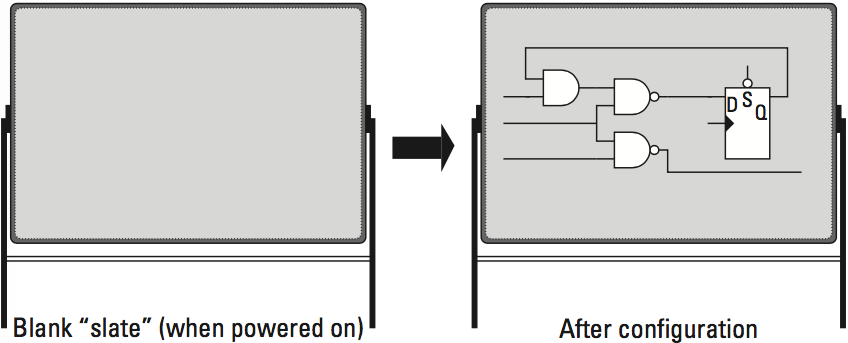
\includegraphics[width=0.9\textwidth]{img/rt-board.png}
        \caption{Ilustração em alto nível do funcionamento interno do FPGA. Fonte: \citet{Sass2010}.}
        \label{fig:rt-board}
    \end{figure}
    
    % o que é um fpga
    %LUTS
    O FPGA constitui-se de vários módulos lógicos pequenos, programáveis, independentes e interconectados para criar funções maiores.
    %Cada módulo lida, normalmente, com até quatro ou cinco variáveis de entrada.
    Utilizam de \textit{Lookup Table} (LuT) para criar as funções lógicas desejadas.
    Uma LuT funciona como uma tabela-verdade onde a saída é programada para representar a função combinacional, armazenando valores verdadeiros e falsos adequado a cada combinação de entrada.
    %Os recursos de roteamento de sinal programável dentro do chip tendem a ser bem variados, com extensões de caminhos diferentes disponíveis.
    %Os atrasos de sinal em um projeto dependem do roteamento real de sinal selecionado pelo \software\ de programação.
    %Os módulos lógicos também contêm registradores programáveis.
    %Eles não são associados a nenhum pino de entrada e saída (I/O, do inglês \textit{Input and Output}).
    %Cada pino de I/O é conectado ao bloco programável de entrada e saída que, por sua vez, é conectado aos módulos lógicos com linhas de roteamento selecionadas.
    Eles reduzem a lista de componentes necessários para o desenvolvimento do projeto, além de simplificar o protótipo, encurtar o ciclo de desenvolvimento e principalmente reduzem o tamanho e os requisitos de potência para o funcionamento do produto \cite{tocci2003sistemas}.
    
    
    
    \subsection{A Tecnologia Reconfigurável e a Plataforma de Manuseio}
    
        %arquitetura
        Uma arquitetura simples de FPGA é exibido na Figura~\ref{fig:rb-arch_fpga}. 
        Nela os quadrados menores situado nas laterais são blocos de I/O que podem ser configurados para fornecer recursos de entrada, saída ou bidirecionais.
        Os quadrados maiores situados no interior são as LuTs, usados para guardar dados que entram ou saem e realizar as operações lógicas.
        Os canais que interligam os blocos entre si são estabelecidas por meio de conexões que passam por linhas e colunas, e possuem a funcionalidade de serem interconexões programáveis \citep{tocci2003sistemas}.
        %A tecnologia interna de um FPGA consiste basicamente de um arranjo de blocos lógicos, canais de roteamento para interconexão de blocos lógicos e blocos de entrada e saída de sinais em torno do circuito.
        Hoje, esses dispositivos possuem milhões de portas de lógica programável, bilhões de transistores, além de outros blocos de \hardware\ dedicados como memórias embarcadas e multiplicadores de ponto-fixo, tornando-o um dos circuitos integrados (CI) mais densos existente \citep{Choi2016}.
        Um projeto terá sucesso de sintetização se ele conseguir ser acordado à quantidade de recursos disponíveis do FPGA e executar rápido o suficiente para concluir seus objetivos sistêmicos \cite{coffman1999real}.
    
        \begin{comment}
        \begin{wrapfigure}{O}{0.5\textwidth} \centering
        %\vspace{-10pt}
        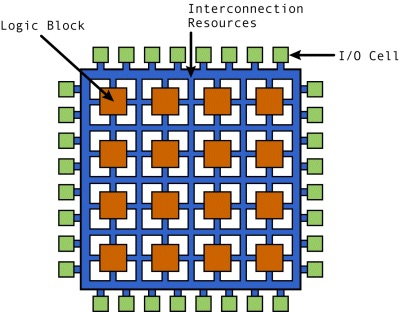
\includegraphics[width=0.5\textwidth]{img/rt-arch_fpga.jpg}
        %\vspace{-15pt}
        \caption{Exemplo em baixo nível da arquitetura internas de um FPGA. Fonte: \url{http://www.eetimes.com/document.asp?doc_id=1274496}. Acesso: 30/05/2018.}
        \label{fig:rb-arch_fpaga}
        \end{wrapfigure}
\end{comment}
        
        \begin{figure}[h] \centering
            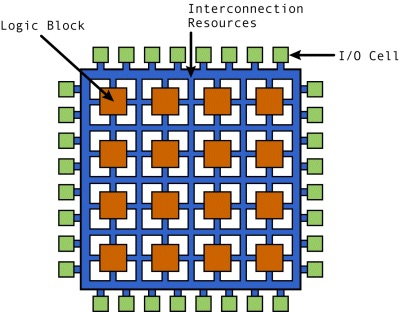
\includegraphics[width=0.65\textwidth]{img/rt-arch_fpga.jpg}
            \caption{Exemplo em baixo nível da arquitetura internas de um FPGA. Fonte: \url{http://www.eetimes.com/document.asp?doc_id=1274496}. Acesso: 30/05/2018.}
            \label{fig:rb-arch_fpga}
        \end{figure}
    
    
    
        % uso de fpga no mundo
        \Hardwares\ reconfiguráveis eram utilizados unicamente na prototipação de projetos de circuitos integrados de aplicação especifica (ASIC, do inglês \textit{Application-Specific Integrated Circuit} e produzido em baixo volume por causa de seu baixo desempenho e custo por unidade.
        Mas com a variedade desses dispositivos disponibilizados hoje no mercado em conjunto com a elevação do custo de pesquisa, \design,\ desenvolvimento e teste e exigências de mercado, houve um crescente interesse na utilização de FPGAs para SE devido suas vantagens sobre ASICs em geral em termos de flexibilidade de projeto e custo e dessa forma dispositivos reconfiguráveis são a tecnologia-chave para o futuro dos sistemas digitais \citep{Mei2000, tocci2003sistemas}.
        
        % Importancia
        \citet{tocci2003sistemas, Plessl2003} citam ainda que o motivo de \hardwares\ reconfiguráveis estarem dominando o mercado é o fato de que, como são dispositivos programáveis, a mesma funcionalidade pode ser obtida ao invés de diversos CI individuais.
        Isso significa maior confiabilidade, menor espaço ocupado na placa, consumo de energia, complexidade de desenvolvimento e, geralmente, menor custo de fabricação.
        
        
    
        % o que é lut
        Ao utilizar a tecnologia \lut,\ o FPGA torna-se versátil para comportar qualquer função digital e também ser eficiente para ser implementado em silício.
        %O controle de entrada de sinais é usado como entrada lógica e o multiplexador de entradas é ligado ao nível lógico para implementar a função desejada \citep{coffman1999real}.
        %
        % o que a sintetização faz
        A ferramenta de sintetização toma o HDL vindo do \designer\ e mapeia-o em \hardware.\ 
        Primeiro o sintetizador irá minimizar equações lógicas removendo termos lógicos redundantes de acordo com seu sistema de optimização e com isso, o \design\ final do projeto será um grande conjunto de equações Booleanas que representa o sistema descrito pelo projetista \citep{coffman1999real}.
       
        
        % tecnologia e energia
        Segundo \citet{tocci2003sistemas}, tais maravilhas de flexibilidade de projetos digitais podem fornecer uma série de opções de projeto sendo voltados para indústria e até mesmo educação.
        Ao utilizar tecnologia como CMOS e SRAM, o consumo de energia do chip é relativamente baixo comparado com outras tecnologias, podendo ser confeccionado em nível de tensão elétrica, frequências e cargas para os sinais de I/O.
        O mercado fornece diferentes FPGAs com graus de velocidade variados a fim de que o projetista utilize o mais adequado ao projeto.
        
        FPGAs rápidos ou com maior número de recursos consequentemente são mais caros e por isso, escolher o FPGA adequado ao projeto também é necessário para obter um bom produto \cite{coffman1999real}.
        %Entretanto, como um dispositivo FPGA pode ser configurado para um número infinito de projetos digitais, isso implica na não possibilidade de afirmar o montante de dissipação de energia para um dispositivo FPGA.
        %O \software\ Quartus II tem duas ferramentas para estimular o montante de uso de energia para uma aplicação.
        %O \textit{PowerPlay Early Power Estimator} é usado durante os estágios iniciais do projeto para estimar a magnitude de potência do dispositivo.
        Dessa forma, FPGAs são chips que podem ser programados instantaneamente para funções de qualquer circuito digital \citep{Choi2016}.
        
        
        
        
        % Plataforma FPGA
        Uma plataforma FPGA é um chip que além de conter o componente FPGA, está integrado à inúmeras interfaces e componentes, desde LEDs (do inglês \textit{Light-Emitting Diode}) e \textit{switchs} até porta Ethernet e interface vídeo VGA (do inglês \textit{Video Graphics Array}) com seus respectivos circuitos.
        Um exemplo de plataforma é exibido na Figura~\ref{fig:rb-arty}.
        Como possui recursos suficientes para circuitos digitais complexos é possível sintetizar por exemplo funções de processamento de imagem, algoritmos de redes de computadores, algoritmos criptográficos e \textit{soft}-processadores completos \citep{Plessl2003}.
        
        \begin{figure}[h] \centering
            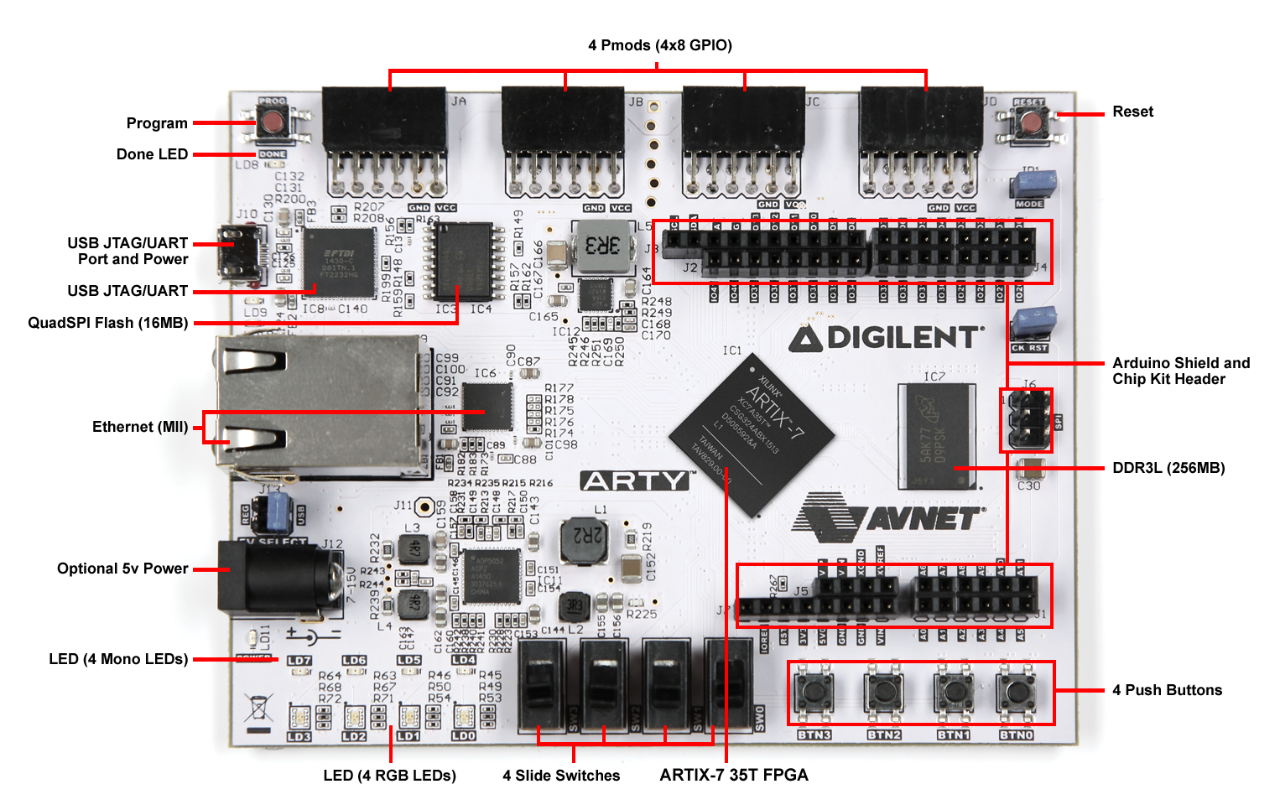
\includegraphics[width=0.99\textwidth]{img/arty.png}
            \caption{Exemplo de uma plataforma FPGA na qual constitui-se de uma placa com o FPGA e seus componentes de interação. Fonte: \url{http://www.xilinx.com/products/boards-and-kits/arty.html}. Acesso: 30/05/2018.}
            \label{fig:rb-arty}
        \end{figure}
   
   
   
    \subsection{Sintetização de Circuitos e Algoritmos no FPGA}
    
    %\subsection{\textit{Hardware Description Language} (HDL)}
        Uma das principais formas de sintetização é utilizando linguagens da classe de Linguagens de Descrição de \Hardware\ (HDL, do inglês \textit{Hardware Description Language}).
        HDL é uma das classes de linguagens de computação usados para descrever formalmente um circuito eletrônico por meio do comportamento temporal ou da estrutura espacial de circuito de um sistema eletrônico, originado pela necessidade de documentar o comportamento do \hardware\ \citep{Sass2010}.
        
        HDL é amplamente utilizada em \design\ de \hardware\ especificando os detalhes de \design\ para qualquer sistema digital, ou seja, tanto para desenvolvimentos de circuitos ASICs quanto para FPGAs.
        Especificado o modelo comportamental de um circuito específico, antes ser projetado e construído, ferramentas lógicas de sínteses são invocadas para gerar informações estatísticas e geométricas que são utilizadas para verificar sua viabilidade.
        %
        Feita as análises, o código é entregue ao compilador lógico chamado de ferramenta de síntese, e sua saída será carregada ao dispositivo reconfigurável, ou seja para suas \luts.\ 
        É possível alterar o código HDL, compilá-lo e fazer sua síntese no mesmo \hardware\ reconfigurável, quantas vezes forem necessárias, sem custo adicional, propriedade única fornecida pela tecnologia da lógica programável \citep{Smith1998}.
        
        Como a maioria dos FPGAs utilizam tecnologia SRAM, eles com isso tornam-se voláteis.
        Isso significa que ao ser energizado, todas as informações de sintetização anteriores se perdem.
        Para contornar este problema, exite também uma memória secundária que guarda as informações de programação que definem como cada bloco lógico comportará, quais blocos serão de entrada e saída, bem como como são as interconexões entre os blocos \cite{tocci2003sistemas}.
                
        Linguagens HDLs como \textit{VHDL} e \textit{Verilog} possuem um nível elevado de complexidade devido suas de naturezas serem linguagem de baixo nível \citep{Choi2016}.
        E para a facilitação do processo de \design,\ existe outra classe de linguagens que permite a sintetização de projetos utilizando linguagens de alto nível \citep{Sass2010}.
        Realizado uma especificação de \design\ em \software, uma Síntese em Alto Nível (HLS, do inglês \textit{High-Level Synthesis}) pode reduzir os longos ciclos do processo de \design\ de \hardware\ e ainda trazer melhoria em desempenho e eficiência energética \citep{Choi2016}.
        Essas linguagens convertem seus códigos em alto nível para HDL e assim realiza-se a sintetização do projeto no \hardware\ reconfigurável.
        
        
        %IP disponibilizados
        Outro item importante na consideração de utilização de FPGA para projetos é a disponibilidade de módulos com propriedade intelectual (IP).
        Este refere-se a projetos predefinidos de módulos complexos usados para satisfazer necessidades de funcionamento do projeto.
        Tais blocos são disponibilizados pelas empresas fabricantes de FPGA ou por fontes terceiras proprietárias destes.
        %
        Dessa forma é possível utilizar módulos completos disponibilizados ou adquiridos a fim de tornar o sistema mais fácil para utilização e robusto.
        Uma variedade de \cores\ IP são disponibilizados para uso em licenciamento barato, na qual são \citep{coffman1999real}:
        \begin{itemize}
            \item Microprocessadores, e \cores\ DSP;
            \item Conversores digitais, GSM e outras formatos e frequências de rádio;
            \item Codificações e decodificações de áudio e vídeo;
            \item Encriptadores e decriptadores PGP e outros algoritmos simétricos e assimétricos;\
            \item DCT, FFT, wavelet e outros cálculos de transformações;
            \item Jogos, \cores\ educacionais e vários outros.
        \end{itemize}
        
        Como o ciclo de vida para produtos está cada vez mais curto por causa do rápido desenvolvimento de tecnologia e recursos, é cada vez mais importante para os desenvolvedores encontrar maneiras de encurtar o ciclo de projeto e desenvolvimento de novos produtos.
        Dessa forma, utilizar de recursos de IP diminuem o tempo necessário ao projetista para concluir seu produto.
    
    
    
    \subsubsection{Otimizações Automáticas de Projeto}
    
        %area e delay optimization
        Segundo \citet{coffman1999real}, a sintetização também realiza otimizações com foco em \textit{delay} e área utilizada.
        O processo é representado como um construtor automático de rotas a partir do HDL, isso é, existe várias formas de fazer a rota de um determinado circuito.
        O processo de sintetização foca em realizar um roteamento que enquadra com os requisitos do \design,\ mesmo se existe a possibilidade de obter melhores resultados em tamanho de área consumida, recursos ou \textit{delay}.
        O resultado da sintetização gerada é avaliada comparando se o sistema gerado é suficiente para ser executado sem erros e isso não significa que o resultado sintetizado gerado será de baixa qualidade pois o \design\ continuará respeitando os requisitos de tempo para seu funcionamento.
        
        Como os conceitos de área e \textit{delay} são inversos entre si, a sintetização mais rápida não buscará ser a menor em espaço e recursos utilizados, da mesma forma que e a busca pela menor área não significará a mais rápida sintetização.
        O quão fácil será a tarefa de sintetização do projeto dependerá de vários fatores como a quantidade de recursos disponíveis do FPGA escolhido para uso, a tecnologia que o FPGA utiliza, os requisitos de velocidade sistêmicos e o \design\ descrito pelo projetista.
    
    
    \subsubsection{Manipulação de Tamanho de Projeto Sintetizável}
    
        %manipulação de tamanho do recurso
        A manipulação do projeto também é passo importante para a quantidade de recursos alocadas a este e qualquer mudança também é substancial.
        Módulos que utilizam grande quantidade de recursos podem ser obter resultados diferentes de sintetização ao quebrar uma rotina em sub-rotinas menores, podendo fazer com que o recurso em \hardware\ fique menor e mais fácil de ser implementado.
        %
        Há três momentos que agregar sub-rotinas também são estratégias inteligentes. 
        Se duas sub-rotinas tomam por exemplo, 25\% cada uma do tempo da aplicação, então elas são fortes candidatas para a implementação em \hardware\ pois usufruem de grande tempo de processamento e este pode ser trabalhado em nível de \hardware. 
        No entanto, se forem implementadas individualmente, cada uma também necessita do custo da sua interface de comunicação com os módulos subsequentes à ela. 
        Se há três sub-rotinas relacionadas (uma invocando a próxima), então a combinação delas pode reduzir o custo de invocações. 
        %Entretanto, o custo da interface não é sempre insignificante e vale a pena o esforço do usuário para investigar a situação.
        
        Da mesma forma, implementações em \hardware\ têm desempenho significativo em usar formatos de dados de dados específicos à sua finalidade. 
        %Para que o \software\ seja mais eficiente nos formato de dados não padronizados, programadores irão investir em estruturas de dados que não são bem mapeadas para o \hardware. 
        Assim, é possível realizar a consideração dos tipos de dados para melhor adaptação ao projeto sintetizado evitando conversões entre níveis \hs\ e com isso explorar melhor o potencial do FPGA visando seu desempenho e recursos utilizados \cite{Sass2010}.
        
        
    \subsubsection{Teste}
        %projedo deve ser pequeno para grande
        O projeto de circuito digital no FPGA deve ser feito a partir do seu modo mais simples, onde escreve-se os trechos de códigos, testá-lo e garantir que ele corresponda à seus requisitos básicos de funcionamento \citep{tocci2003sistemas}.
        
        %teste
        O projetista realiza testes nos módulos construídos visando abordar todos os estímulos possíveis e verificar se a resposta se adéqua às entradas.
        Dessa forma, ao garantir que as pequenas partes funcionam, ao conectá-los, tem-se que o conjunto deles também funcionarão \citep{tocci2003sistemas}.
    
    
    
    \subsection{CSoC}
        É possível também realizar a integração de um controlador/processador à tecnologia FPGA.
        Sistemas que possuem um sistema computacional integrado à uma única placa na qual inclui um FPGA possui o nome Sistema em Chip Configurável (CSoC, do inglês \textit{Configurable System on a Chip}).
        
        Ao utilizar deste sistema, a plataforma FPGA será constituída de uma arquitetura semelhante à exibida na Figura~\ref{fig:rb-soc} onde as setas representam os barramentos de comunicação entre os principais componentes.
        
        \begin{figure}[h] \centering
            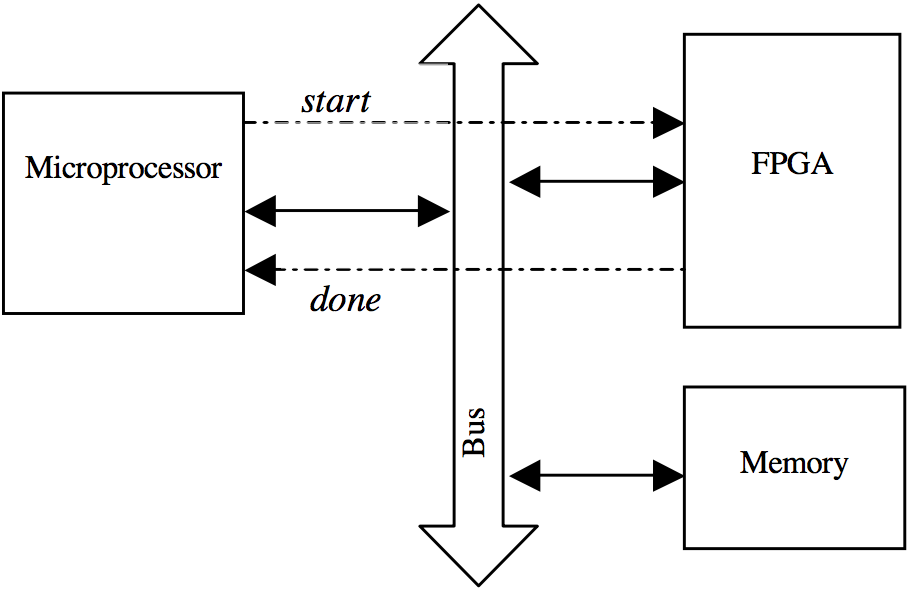
\includegraphics[width=0.7\textwidth]{img/into-soc.png}
            \caption{Visão geral de um SoC FPGA.}
            \label{fig:rb-soc}
        \end{figure}
    
    
        % Utilização de um processador sintético ou físico
        A unidade de processamento central nesses tipos de sistemas pode ser utilizada/implementada de duas formas, sendo estas \textit{hard} e \textit{soft} \cores.
        %
        %hard
        O processador \textit{hard core} é um \core\ fisicamente dedicado. Isso significa que é um um pedaço de CI que pode estar dentro do próprio circuito de um FPGA ou integrado à sua plataforma de componentes na qual possui um barramento para a comunicação.
        Este sistema não utiliza de recursos do FPGA para a utilização do processador.
        %soft
        Já o processador \textit{soft core} é implementado por meio da sintetização e mapeamento de um modelo de um processador no FPGA.
        Dessa forma, ao invés de ter um circuito de um processador independente dos componentes da plataforma, tem-se a sintetização deste dentro do FPGA por meio das \luts.\ 
        Assim, o FPGA deve realizar a construção do sistema completo utilizando seus recursos de construção de circuitos digitais na qual passam pelo mesmo processo das demais sintetizações sendo elas \design\ mapeamento e sintetização na placa.
        
        Cada um tipo de \core\ possui suas vantagens.
        Ao utilizar um \textit{hard} \core, é possível utilizar todos seus recursos obtendo máximo desempenho nas atividades executadas, a utilização de um \textit{soft} \core\ permite a extensão da arquitetura \citep{Plessl2003}.
    
    
        \subsubsection{Processadores \textit{Soft Core}}
        
            %geral
            Devido ao grande aumento do número de microprocessadores na qual podem ser integrados em vários SoC de grande porte que necessitam de robustez, percebeu-se que havia a necessidade de microprocessadores modificáveis. % \citep{kranenburg2010mb}.
            %
            Com o aumento da capacidade dos FPGAs foi possível a construção desses componentes tanto comerciais quanto \textit{open source} em sistemas SoC, utilizados em aplicações que variam desde computação paralela até rede de computadores \citep{kranenburg2010mb}.
            
            % hard e soft
            Um processador \textit{hard core} fabricado não possui nenhuma forma de reconfiguração da lógica de seus dispositivos ASIC.
            Qualquer mudança necessária num projeto desses dispositivos seria necessário realizar uma nova construção da máscara litográfica e uma nova fabricação deste, processo longo e custoso.
            E também quando o sistema baseado em processador com suas instruções customizadas já foi mapeado em um ASIC, a única possibilidade de mudança da aplicação deveria ser realizada em nível de \software,\ alterando seu código.
            %
            Já processadores \textit{soft cores} integram a instrução customizada completamente em suas unidades de execução e são úteis se um determinado \hardware\ não é moldável como são os ASICs.
            Utilizando FPGA como meio para esses SoC nos permite a reconfiguração da lógica interna de forma fácil rápida e barata, isso em qualquer estágio de construção do projeto \citep{rosinger2004connecting}.
        
            % vantagens do soft
            Uma das vantagens do uso de um processador \textit{soft core} é a sua flexibilidade.
            Essa propriedade de projetos de nível alto permite que projetista utilize apenas os recursos realmente necessários do processador para sua aplicação específica.
            Além disso, essa característica também permite que esses processadores sejam facilmente integrados com módulo de IP resultando num processo mais rápido no desenvolvimento de um projeto e um produto final sólido \citep{rosinger2004connecting}.
        
        
        
        
            %microblaze
            MicroBlaze\texttrademark\ é uma família de configurações comerciais predefinidas de um RISC de 32 bits utilizados como módulo IP em desenvolvimento de projetos em FPGA com \textit{soft}-processadores. 
            Ao adicionar o processador ao projeto, é possível utilizar \softwares\ de desenvolvimento que não necessitam de experiência prévia em \hardware\ reconfigurável para desenvolver aplicações para o processador MicroBlaze. 
            O processador MicroBlaze atende aos requisitos de diversas aplicações, incluindo os mercados Industrial, Médico, Automotivo, Consumidor e de Comunicações pois ele possui configurações que suportam o comportamento para classes de processadores em tempo-real, para aplicações em geral e microcontrolador.
            
            % arquitetura
            Ele possui um conjunto de instruções de 32-bit e registradores de propósito geral, além barramento de 32-bits, expansível par 64.
            É possível também incluir unidade de ponto flutuante, permitindo o uso do processador adequando melhor ao projeto.
            Possui suporte à \textit{pipeline} na decodificação de instruções, bem como suporte à interface de comunicação AXI \citep{obeidat2011microblaze}.
            
            
            %microblaze e open source
            Diferentemente de processadores \textit{open source}, MicroBlaze possui qualidade no componente disponibilizado, suporte e documentação disponíveis para o desenvolvedor.
            Muito dos \designs\ \textit{open source} são difíceis de serem modificados devido sua complexidade, além da falta de uma metodologia de \design\ ou a ausência de documentação clara.
            Além de que muitos destes processadores não são portáveis e funcionarão em modelos específicos de FPGAs.
            %
            Processadores comerciais são constantemente escolhidos para uso devido ao fato de terem um preço relativamente barato ao concorrentes e que estes podem ser facilmente acoplados à um projeto sintetizável em FPGA \citep{kranenburg2010mb, kranenburg2009reference, rosinger2004connecting}.
            
            Também é possível construir uma arquitetura básica de um MicroBlaze multi core.
            Instancia-se vários MicroBlazes cada um com memória local privada e todos conectados ao barramento \textit{Open Core Protocol} (OPB) e com isso cada processador tem uma conexão \textit{full-duplex} com os outros MicroBlaze, e uma descrição da arquitetura é exibida na Figura~\ref{fig:rb-multi}  \citep{xu2008multi}.
            
            \begin{figure}[h] \centering
                %\vspace{5pt}
                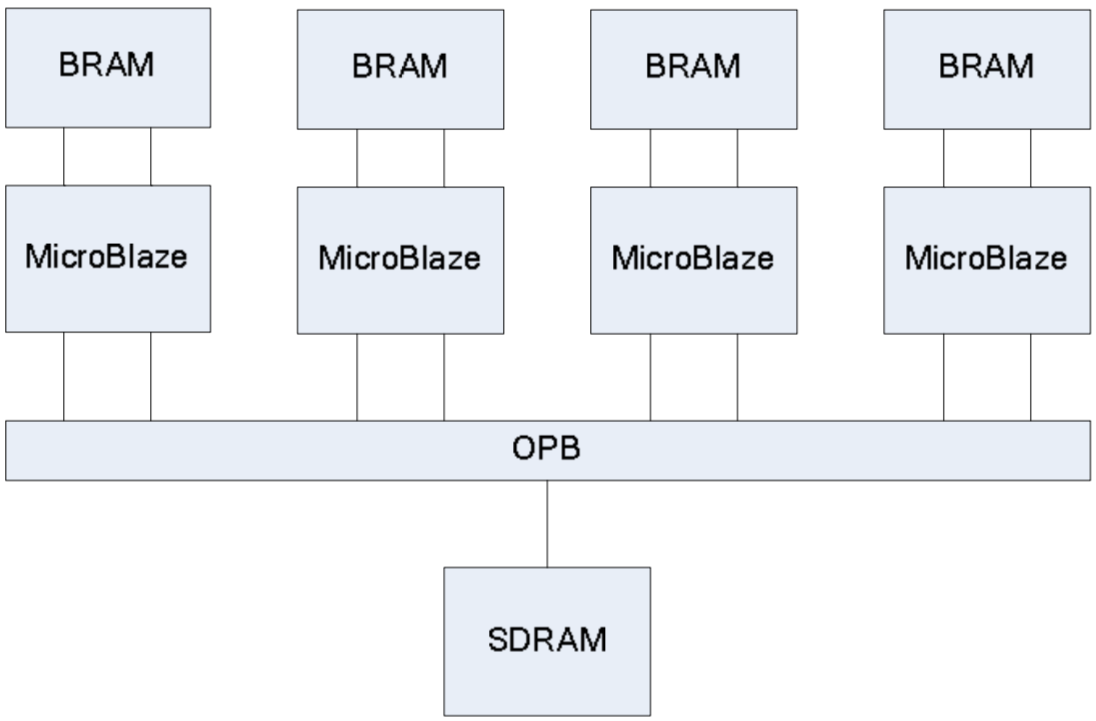
\includegraphics[width=0.7\textwidth]{img/rb-multi-microblaze.png}
                %\vspace{15pt}
                \caption{Esquema de multi-MicroBlazes. Fonte: \citep{xu2008multi}.}
                \label{fig:rb-multi}
            \end{figure}
            
            
            Há diferentes formas de conectar um módulo IP em um processador \textit{soft core}.
            Cada aplicação pode ser realizada e implementada tanto como um algoritmo em \software\ quanto num \hardware\ estrutural como é exibido na Figura~\ref{fig:rb-mb-hs}.
            Neste exemplo, uma mesma porção de código implementado tanto em \hs\ possui diferentes desempenhos.
            Ao utilizar uma implementação em \software\ tem-se seu código sequencial executado pelo processador e na transformação deste em um módulo de \hardware\ pode executá-lo como um módulo dedicado e ainda aplicar otimizações de \hardware\ \citep{rosinger2004connecting}.
            
            \begin{figure}[h] \centering
                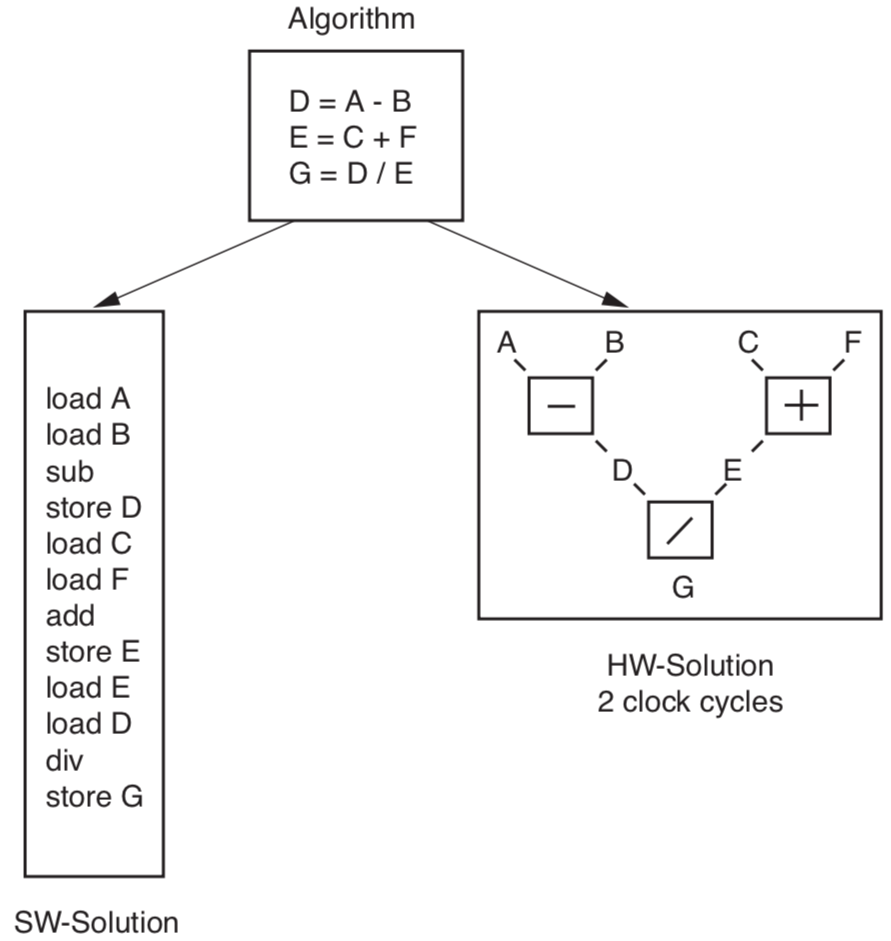
\includegraphics[width=0.67\textwidth]{img/mb-hs.png}
                \caption{Comparação hipotética de implementações em \software\ e \hardware\ com otimizações.}
                \label{fig:rb-mb-hs}
            \end{figure}
            
            Este também permite ao usuário escrever \textit{firmwares} customizados em Verilog e VHDL que atribui ao processador um barramento local permitindo que o projeto possua interface de comunicação com quase todos os dispositivos conectados como sensores, atuadores, sistemas heterogêneos providos externamente \citep{kranenburg2010mb}.
        
            Ao adicionar o processador \textit{soft core} MicroBlaze junto do barramento AXI, o projeto assistido pelo computado será semelhante ao circuito digital exibido pela Figura~\ref{fig:rb-mb}.
            Exibe-se os blocos formados por módulos IP e seus componentes complementares necessários para o funcionamento básico do projeto como memórias e \textit{clocks}.
            
            \begin{figure}[h] \centering
                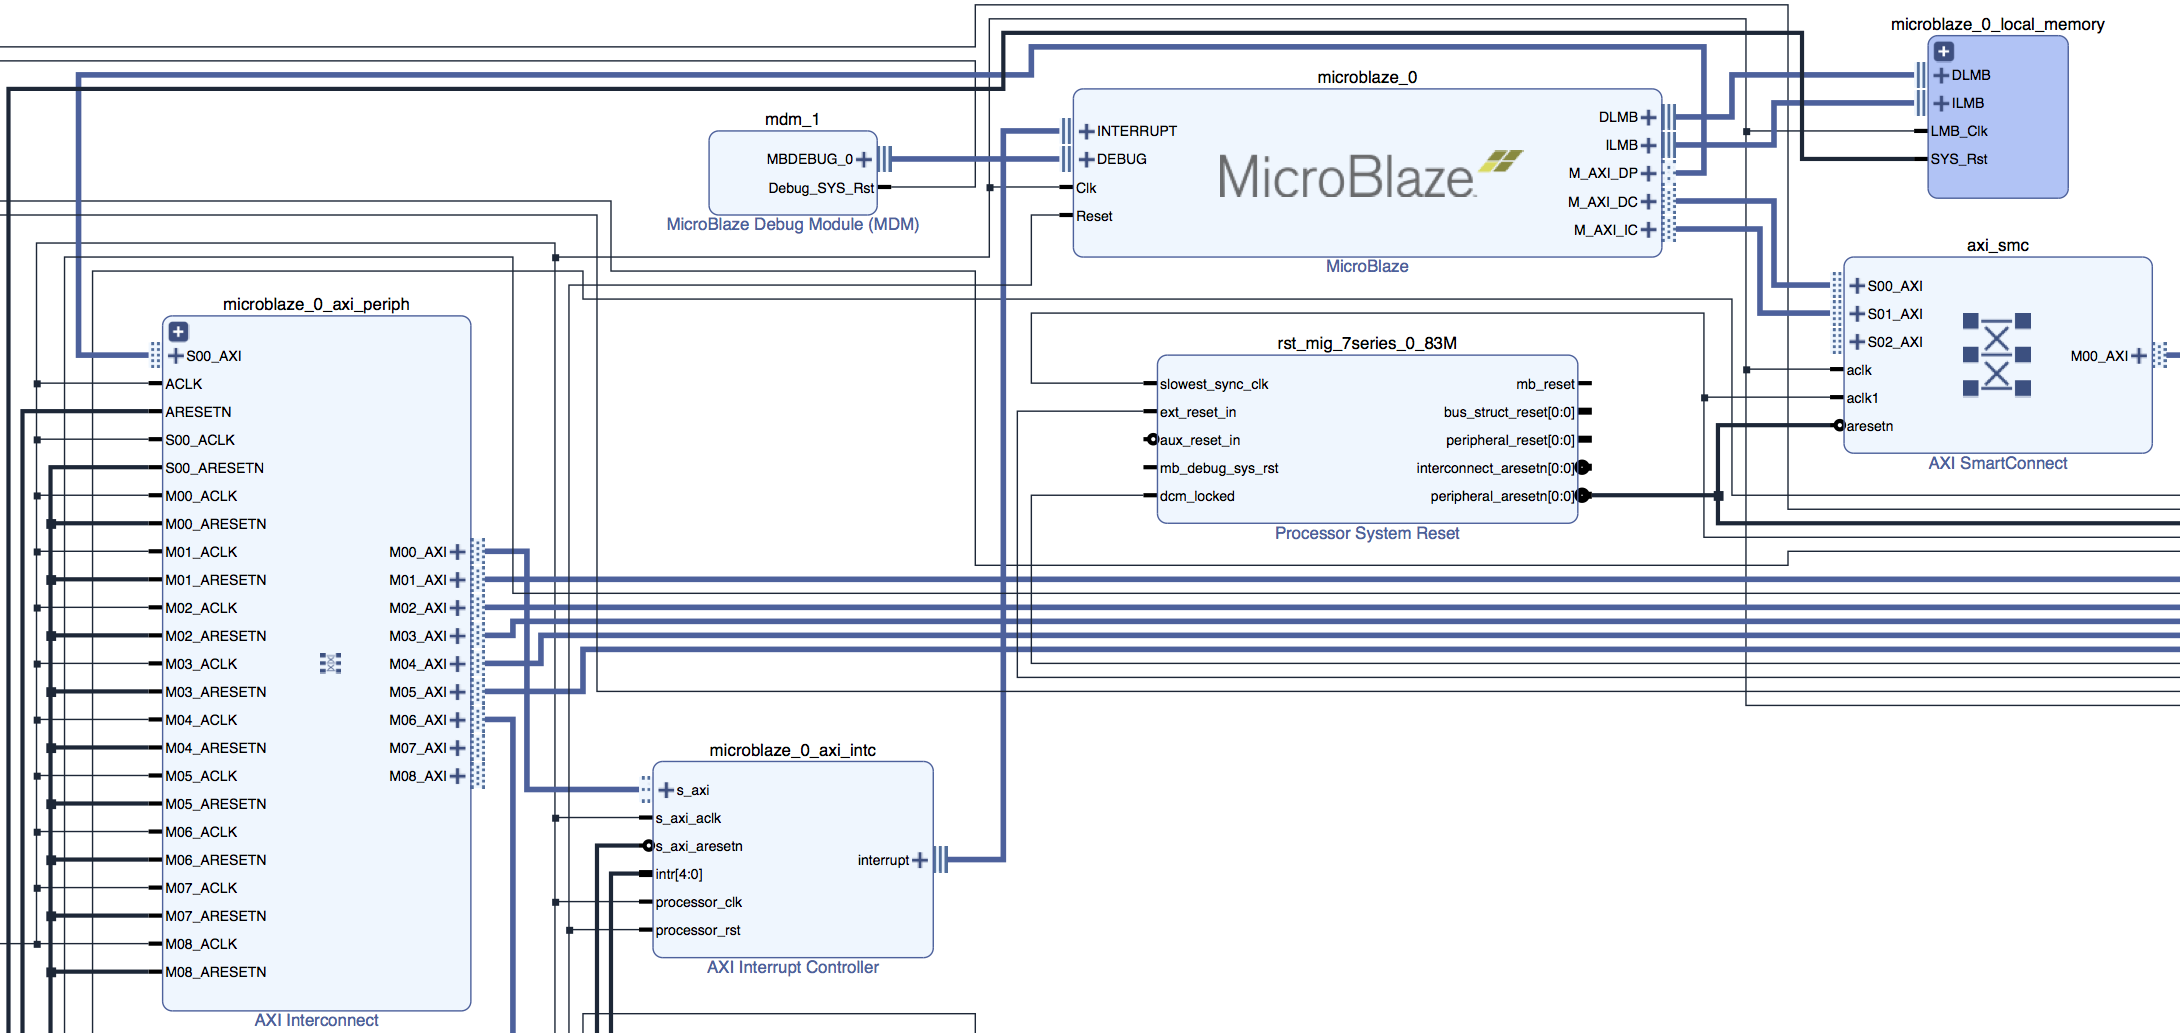
\includegraphics[width=1.0\textwidth]{img/1-microblaze-axi.png}
                \caption{Visão geral do MicroBlaze com o barramento AXI já integrado ao projeto.}
                \label{fig:rb-mb}
            \end{figure}
        
        



\begin{comment}
\section{\Profile} \label{sec:profile}

		\Profile\ é uma procedimento para auxiliar o usuário a coletar informações do \software\ em tempo de execução.
      Existem vários programas diferentes para adquirir essas informações e podem ser distinguidos em duas categorias.
      A primeira é aqueles que apresentam a quantidade de declarações e invocações de rotinas, e aqueles que exibem informações de tempo de declarações e rotinas \citep{nemeth2004manual}. Um exemplo de saída é exibida a seguir.

{ \footnotesize
      \begin{verbatim}
Flat profile:

Each sample counts as 0.01 seconds.
  %   cumulative   self              self     total
 time   seconds   seconds    calls  ms/call  ms/call  name
 33.34      0.02     0.02     7208     0.00     0.00  open
 16.67      0.03     0.01      244     0.04     0.12  offtime
 16.67      0.04     0.01        8     1.25     1.25  memccpy
 16.67      0.05     0.01        7     1.43     1.43  write
 16.67      0.06     0.01                             mcount
  0.00      0.06     0.00      236     0.00     0.00  tzset
  0.00      0.06     0.00      192     0.00     0.00  tolower
  0.00      0.06     0.00       47     0.00     0.00  strlen
  0.00      0.06     0.00       45     0.00     0.00  strchr
      \end{verbatim}
      \vspace{-3em}
}

      \begin{wrapfigure}{o}{0.56\textwidth} \centering
         %\vspace{15pt}
         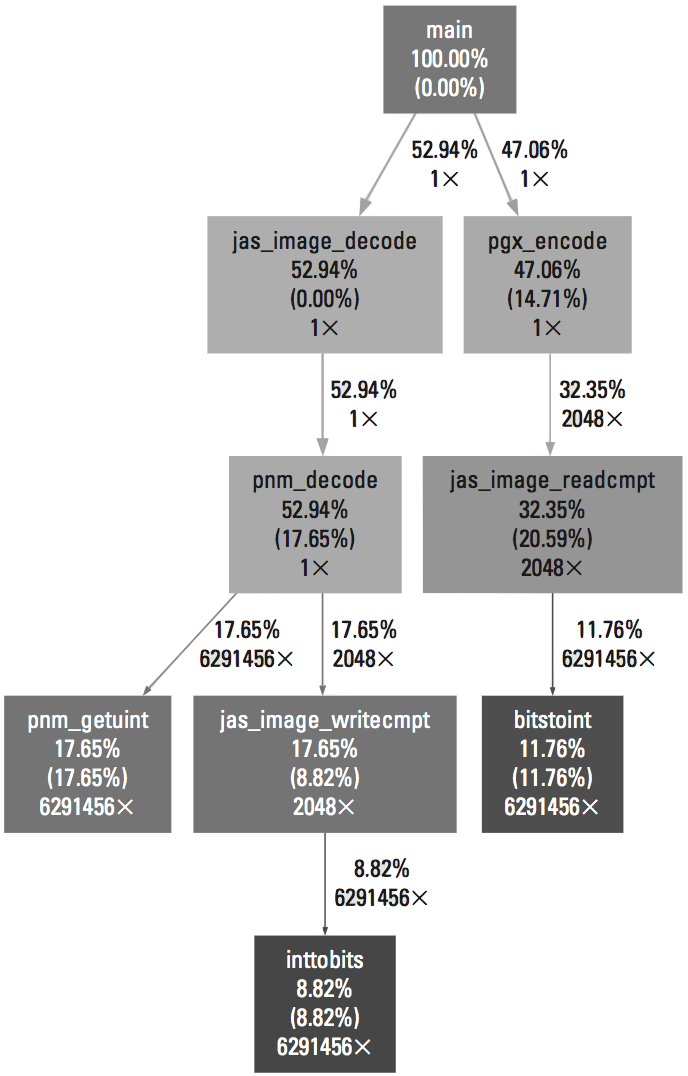
\includegraphics[width=0.48\textwidth]{img/f4-1-2.png}
         %\vspace{-1em}
         \caption{\Profile\ da codificação de imagem em formato JPEG. Fonte: \cite{Sass2010}. \vspace{-0em} }
         %\vspace{-3em}
         \label{fig:profile}
      \end{wrapfigure}

      A Figura \ref{fig:profile} exibe um exemplo gráfico de \profile\ de \software\ em um codificador de imagem em formato JPEG.
      O processo é feito ao colocar o \software\ referencial (programa a ser coletado) como entrada representativa na ferramenta e a coleta é realizada em várias partes da aplicação ao longo de sua execução neste.
		Uma das técnicas do \profile\ de mensurar uma aplicação é na realização de interrupções periódica no programa e amostrar o seu \textit{program counter}.
      Dessa forma, é possível utilizar um histograma para contar quando um programa é interrompido em um endereço particular e a partir dessa informação, calcular a fração aproximada do tempo total de execução gasto em suas partes.
      Distribuições GNU/Linux possuem a ferramenta \texttt{gprof} na qual avalia procedimentos enviados por parâmetro, realizando o cálculo de tais informações de \software\ \citep{Graham1982}.
\end{comment}



\section{Sistemas Computacionais \Wearables}

    %\subsection{Definição}
    
        \citeauthor{starner1996human} em \citeyear{starner1996human} descreveu sistemas computacionais \wearables\ como sistemas que são caracterizados pela sua habilidade de reconhecer o ambiente ao seu redor e comportamentos de seus usuários bem como a situação que os envolvem, e que com esse nível de acesso à informação computacional, revolucionará como os computadores seriam usados.
        Mesmo que esses sistemas ainda eram volumosos e inconvenientes por conta de vários fatores, vários cientistas sustentam essa definição base sobre dispositivos \wearables.\ 
    
        %computadores acoplado ao corpo
        %introdução de que são cheio de sensores e atuadores
        Segundo \citet{Amorim2017, billinghurst1999wearable}, sistemas computacionais \wearables\ são sistemas que com a possibilidade de ter um computador acoplado ao corpo, proporcionam ao usuário um nível superior de informações contextualizadas dentro de um ambiente interativo, podendo ser qualquer dispositivo desde sistemas integrados ao pulso do usuário até mochilas com computadores embutidos.
        Ou seja, são sistemas carregados de sensores e atuadores, acoplados ao corpo, e que proveem medição contínua de parâmetros fisiológicos do usuário ou do seu ambiente ao redor \citep{son2014multifunctional}.
        %
        %deve ser usado em roupa
        % locais que podem ser usados
        %tipo de informações coletadas
        \citet{arias2015privacy} cita que a tecnologia \wearable\ utiliza do pressuposto que deve ser usada em roupas ou acessórios e faz parte de um grande movimento também referenciado como auto quantificado (do inglês \textit{quantified self}).
        Isso refere-se ao autoconhecimento através de números, propriedade permitida pelo seu uso.
        
        Definições mais formais como a de \citet{Gemperle1998} diz que um produto só pode ser considerado \wearable\ se ter a propriedade chamada `\textit{wearability}', sendo esta definida como a interação entre o corpo humano e o objeto \wearable\ estendendo-o em movimento devido à necessidade de movimentação do usuário.
        Esta mesma propriedade está relacionada a objetos mundanos que usamos cotidianamente como roupas e acessórios que não são inteligentes.
        %
        \citet{VanLaerhoven2002} afirmam que a distribuição de elementos computacionais como sensores em objetos mundanos em nosso cotidiano adéqua-se à pesquisa denominada por computação ubíqua e que isso também aplica à computação \wearable,\ uma vez que superfícies de roupas também pode ser uma plataforma de suporte ideal para uma grande quantidade de sensores sendo que estes devem ser miniaturizados para que eles não obstruam seu usuário em seu uso.
        %
        Já \citet{Jozwiak2017} define e caracteriza um sistema computacional \wearable\ como um sistema \textit{cyber}-físico móvel autônomo.
        Em outras palavras \textit{cyber-} é uma combinação dos termos `dispositivo computacional', `rede de computadores' ou `realidade virtual' com um segundo termo, no caso o `físico' oriundo de circuitos.
        
        
        
        %falando + de sensores e atuadores
        Sensores provem um sistema nervoso para detectar sinais.
        Para dispositivos \wearables\ passivos, a existência de sensores é essencial.
        Já atuadores agem uma vez detectado sinais de forma autônoma ou a partir de uma unidade central de controle e assim sendo elementos essenciais para um dispositivo inteligente ativo \citep{starner1996human}.
        %
        Isso significa que tais dispositivos registram e reportam informações sobre o ambiente situado, podendo ser desde avaliação de atividades físicas até padrões de sono.
        Esses dispositivos podem educar e motivar indivíduos a fim de terem melhores hábitos, saúde e segurança, por exemplo \citep{patel2015wearable}.
        %
        As informações coletadas podem variar desde um simples batimento cardíaco e dados de temperatura e umidade até dados sensíveis como a localização atual do próprio usuário e seus hábitos cotidianos de vida.
        
        
        %sistema wearable
        É exibido na Figura~\ref{fig:into-wearable} uma ilustração de um sistema \wearable\ hipotético composto por vários itens como 
        sensores espalhados em seu corpo que ao movimento do usuário são estimulados e geram informações à central, ou 
        componentes atuadores \textit{piezo-electric} integrados ao sapato energizando o sistema \wearable\ com o caminhar \citep{VanLaerhoven2002, Kern2002, Kymissis1998}.
        
        \begin{figure}[h] \centering
            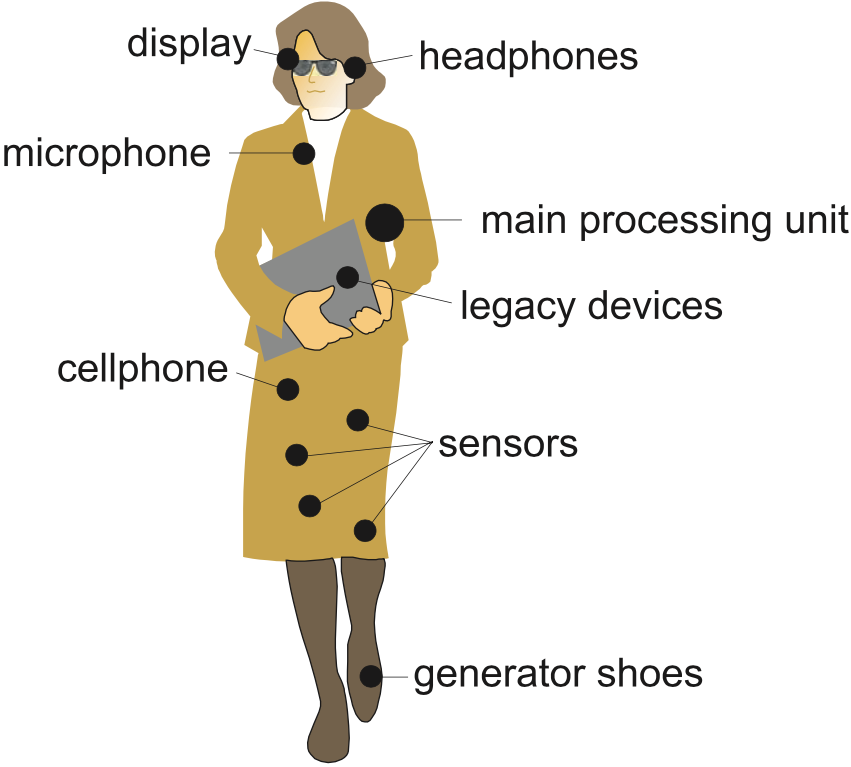
\includegraphics[width=0.66\textwidth]{img/into-wearable2.png}
            \caption{Exemplificação de alguns tipos de dispositivos \wearables.\ Fonte: \citet{Plessl2003}.}
            \label{fig:into-wearable}
        \end{figure}
        
        
        
        \begin{comment}
        %desempenho
        Sistemas \wearables\ executam de tarefas de computação intensiva que consideram restrições de tempo-real onde não realizando-as, o sistema torna-se inaplicável.
        Assim, requere-se um desempenho que seja viável para a execução de suas tarefas.
        % energia
        Da mesma forma, é essencial em um sistema manter-se ativo e funcional num certo período de tempo.
        O \design\ do gasto de energia de um sistema conduz inúmeros desafios e gerenciar esse gasto energético também é um item a ser considerado na construção de um produto.
        Ao alterar os padrões de desempenho de um sistema, seu padrão energético também é alterado \citep{Plessl2003}.
\end{comment}
     
    
    \subsection{Características Funcionais de um \Wearable}
    
        A caracterização de um dispositivo computacional \wearable\ é feita acordando as classificações pré-estabelecidas relacionadas à suas funcionalidades e requisitos de \hardware.
        
        O mercado possui um número considerável de dispositivos \wearables\ que são utilizados em inúmeras áreas, e mesmo que cada equipamento separado tenha suas próprias características, muitas soluções em \hardware\ compartilham uma arquitetura e organização interna de recursos implementados comum.
        Esses detalhes também podem ser expandidos às características relativas à recursos de sistemas operacionais, no qual dispositivos \wearables\ podem ser classificados além de seus componentes de \hardware\ internos como suas funções de desempenho \citep{Delabrida2016, Amorim2017}, como representado pela Figura \ref{fig:classification}.
        
        \begin{figure}[h] \centering
            %\vspace{5pt}
            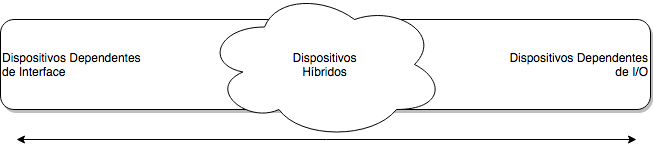
\includegraphics[width=0.97\textwidth]{img/rt-gradiente.png}
            %\vspace{15pt}
            \caption{Classificação de sistemas \wearables. 
                De um extremo existe os dispositivos dependentes de interfaces de usuário e do outro os dependentes de entrada e saída de sinais enquanto entre eles, a gama de combinações possíveis. Fonte: Adaptado de \citep{Amorim2017}.}
            \label{fig:classification}
        \end{figure}
        
        De um lado existem os dispositivos dependentes de interfaces de usuário que possuem alta dependência de operações que fazem referência à comunicação de informação e interação ao usuário sobre sua situação, dessa forma, tais dispositivos provê respostas sobre as interações do usuário.
        Focam principalmente em tarefas para renderização em \textit{displays} como por exemplo equipamentos de realidade virtual e aumentada para implementação de objetos tridimensionais.
        
        De outro lado, existem os dispositivos dependentes de entrada e saída de sinais. 
        Atuam principalmente com o estímulo por algum dado oriundo de outro dispositivo ou do ambiente situado, enviando este dado interpretado à uma nuvem respeitando restrições de tempo-real.
        Isso se da pela utilização de sensores acoplados ao \wearable\ que podem exigir uma boa vazão de dados e pequena latência como são os monitores de atividade remota, situação na qual cria-se o ambiente perfeito para o termo conhecido por IoT (do inglês \textit{Internet of Things}).
        
        Entre dispositivos dependentes de interfaces de usuário e dispositivos de entrada e saída de sinais existe os dispositivos que possui a característica de serem híbridos. 
        São dispositivos que sua natureza é executada sobre características de ambos os extremos citados.
        Dispositivos como \textit{smartwatches} e \textit{fitness trackers} são exemplos de tais dispositivos híbridos, onde possuem restrições de equalização à prioridade dada pelo dispositivo para ambas as operações de interface com o usuário e manipulação de sinais de entrada e saída.
        
        A separação dos conceitos computação \wearable\ e IoT ainda não estão claros segundo a bibliografia científica.
        Sistemas operacionais de propósito específico para ambientes \wearable\ são comumente focado em um único tipo de seguimento de produto como os \textit{smartwatches}, sendo que proporciona aos desenvolvedores um meio para sua aplicação final além de entregar um produto de alta qualidade.
        Também, atualmente, não existe nenhum sistema que satisfaça todos os requisitos apresentados \citep{Amorim2017}.
        
        

    
    \subsection{Miniaturização e Consumo Energético}
    
        %introdução
        O meio científico já estuda \wearables\ há várias décadas como é reportado em trabalhos científicos de \citet{Sutherland1968}, \citet{Mann1996} e \citet{Mann1997}.
        Entretanto, sua comercialização só foi realizada após a miniaturização dos componentes eletrônicos bem com a melhoria na eficiência energética dos mesmo.
        Esse fenômeno fica claro na percepção do crescente espaço ganho recentemente pelos \textit{smartwatches}, \textit{fitness trackers}, óculos inteligentes, equipamentos de realidade virtual e aumentada e outros nas indústrias e nas atividades pessoais de usuários.
        
        %tamanho e qualidade
        Essa restrição de tamanho geralmente significa que a própria qualidade do equipamento também está comprometida, o que leva ao projetista utilizar de muitos atuadores e sensores simplistas no \design\ de um novo produto \citep{VanLaerhoven2002}.
        
        Dispositivos móveis necessitam de sistemas de energização inteligente para seu funcionamento.
        %
        Entretanto, baterias adicionam ao seu projeto tamanho, peso e inconveniência.
        Sobre isso, várias pesquisas foram realizadas de forma a aproveitar o consumo de energia para que o produto possa operar por um período de tempo maior e com a interação mais fluída com o usuário \citep{starner1996human}.
        
        
        Também existe sistemas \wearables\ que são construídos por meio de \textit{electronic textiles}, também conhecidos como, \textit{e-textiles} na qual são fabricações que interconectam eletrônicos em tecidos.
        É possível entregar um produto fisicamente flexível e um tamanho que tipicamente não pode ser alcançado facilmente com outras técnicas de fabricação eletrônicas.
        Com esse tipo de construção, os componentes e suas interconexões são menos visíveis e não suscetíveis a se emaranhar em objetos ao seu redor ou atrapalhar a experiência do usuário.
        Também são facilmente adaptados às rápidas mudanças em tecnologias computacionais e sensoriais de aplicações específicas \citep{starner1996human}.
        
        
        %Comunicação
        Como seu sistema pode ser composto por um conjunto de nós distribuídos, utiliza-se de uma rede de comunicação centralizada num módulo principal realizando a troca de informações entre esses dispositivos.
        Quanto mais dispositivos e componentes como sensores e atuadores conectados no projeto, mais a comunicação torna-se necessária para projeto do sistema e consequentemente mais complexo ele fica.
        Com isso, tem-se então um computador embarcado em um ambiente \mobile\ interagindo com o ambiente ao seu redor, e caso o sistema possua vários nós, a comunicação sem-fio tende a ser a tecnologia predominante por causa da necessidade de mobilidade \citep{Plessl2003,VanLaerhoven2002, Kern2002, Kymissis1998}.

        
        % desempenho e gasto energético
        Como esses dispositivos representam uma parte da heterogeneidade da classe de SE, também estão sujeitos às várias restrições de \design\ relacionadas à classe maior, sendo elas desempenho e gasto energético consciente \citep{Plessl2003, Jozwiak2017}:
        
        \begin{description}
            \item[Desempenho:] 
            %desempenho
            Sistemas \wearables\ executam de tarefas de computação intensiva que consideram restrições de tempo-real onde não realizando-as, o sistema torna-se inaplicável.
            Assim, requere-se um desempenho que seja viável para a execução de suas tarefas;
            
            \item [Gasto Energético:]
            % energia
            Da mesma forma, é essencial em um sistema manter-se ativo e funcional num certo período de tempo.
            Como a eficiência energética está relaciona ao total de energia necessário para computar uma tarefa, o \design\ do gasto de energético de um sistema conduz inúmeros desafios.
            Gerenciar esse gasto também é um item a ser considerado na construção de um produto.
            Ao alterar os padrões de desempenho de um sistema, seu padrão energético também é alterado;
           
            \item [Flexibilidade:] Considera-se o fato de que o dispositivo por ter sua \textit{wearability}, deverá ser utilizado em situações altamente dinâmicas.
            Isso fica claro na necessidade na qual os requisitos de aplicação variam de acordo com as escolhas do usuário, mas também com o contexto e local utilizado.
            Outro, é no fato de que o usuário troca de roupas constantemente e com isso os dispositivos devem ter a capacidade de serem acoplados e removidos, neste caso.
            
            E também, deve-se lembrar de requisitos básicos de todos os embarcados, isso é, critérios como confiabilidade, disponibilidade e fatores dependentes de sua forma como volume e peso.
        \end{description}
        
    
    
    \subsection{Aplicações}
    
        %intro
        \Wearables\ eram utilizados inicialmente para fins de tecnologia militar.
        Ao serem introduzidos ao público, estes equipamentos começaram como itens de elegância e atualmente suas aplicações são voltadas para cuidados com a saúde e áreas da medicina, mostrando como o uso desses dispositivos é possível detectar ou auxiliar o usuário na melhora de hábitos quanto para auxílios na execução de tarefas específicas em uma empresa, por exemplo \citep{chan2012smart}.
        
        As áreas são as mais diversas como por exemplo para consumidores (computação móvel) que são extensões ou reposições de capacidades humanas, para sistemas sociais (\textit{health-care} inteligente), automotivo, industrial (monitoramento) e aplicações comerciais como realidade aumentada para informações turísticas.
        %
        Também é factível que \wearables\ possam ter mobilidade inerente ou ser transportados para outros sistemas, industriais ou naturais (incluindo humanos), sendo autônomos em termos de funcionalidade \citep{Jozwiak2017}.
    
        %ajuda em saúde    
        Algum dos dispositivos são fabricados para indivíduos que já são motivados pela mudança de hábito ou que são considerados para operarem em saúde e seguridade de organizações, empregados, segurança e clínicos com a motivação de melhorarem o desempenho dos respectivos usuários.
        Muito dos comportamentos para uma boa saúde e segurança poderiam ser direcionados para uma melhora significativa na saúde da população se tais dispositivos fossem utilizados com frequência e sem interrupções nas atividades \citep{patel2015wearable}.
        
        
        % podem trabalhar com smartphone
        Não só podem trabalhar de forma autônoma mas também podem serem um artefato de um sistema inteligente maior como computadores, \textit{smartphones} ou até mesmo computação na nuvem, criando cada vez mais um sistema mais inteligente, complexo e interativo com o usuário ou com a demanda da empresa \citep{Jozwiak2017}.
        Uma plataforma sensorial composta de uma luva inteligente para medições multiparamétricas do sistema nervoso, possibilitando o estudo de status cognitivo e físico é exibida na Figura~\ref{fig:health}.
        
        \begin{figure}[h] \centering
            %\vspace{5pt}
            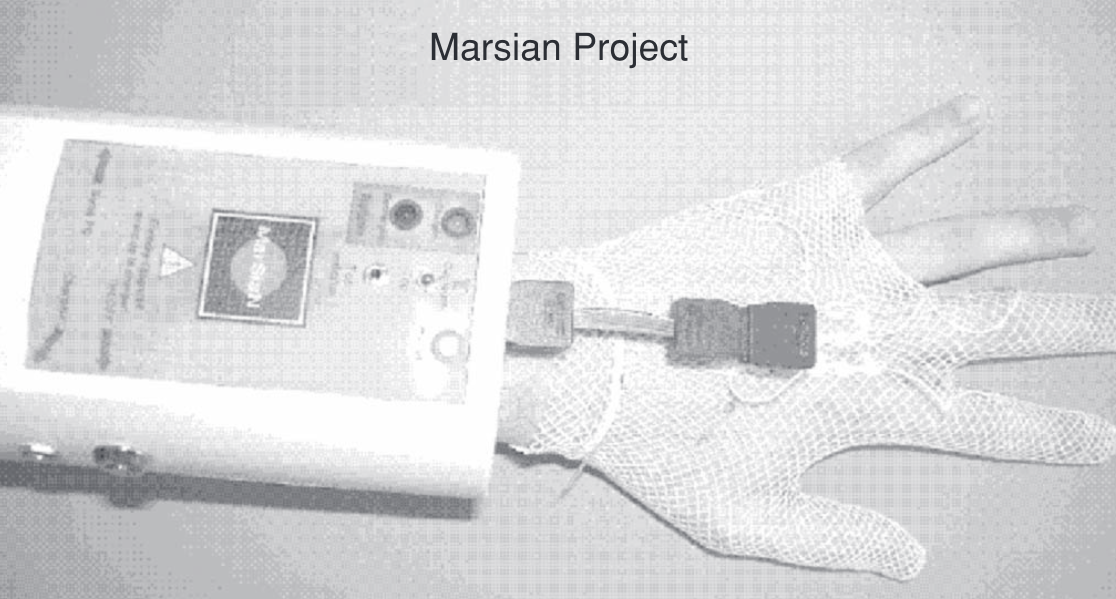
\includegraphics[width=0.8\textwidth]{img/rb-health.png}
            %\vspace{15pt}
            \caption{Ambulatório \Wearable.\ Uma instrumentação ambulatorial composta de roupas, luvas e dispositivo de pulso. Fonte: \citet{lmberis2007advanced}.}
            \label{fig:health}
        \end{figure}
    
        % ajuda em atividades
        Ao utilizar um dispositivo \wearable\ é possível também auxiliar e principalmente melhorar o desempenho de usuários nas mais diversas aplicações como por exemplo manutenção de aeronaves, assistência de navegação e inspeção veicular \citep{billinghurst1999wearable}.
        Um exemplo de interação que possível com o uso de \textit{smartphones} é exibido na Figura~\ref{fig:rb-routine} onde investigou-se o efeito de
        frequência de amostragem de auto-relatos de duas atividades de rotina, sendo elas sentar e andar.
        
        \begin{figure}[h] \centering
            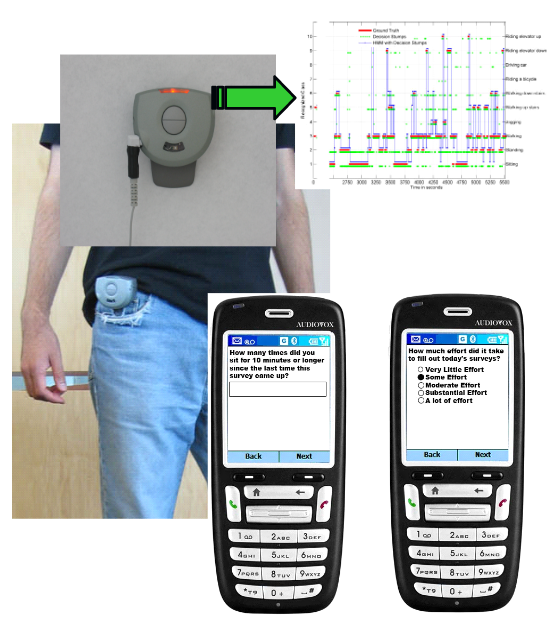
\includegraphics[width=0.7\textwidth]{img/rb-routine.png}
            \caption{Plataforma sensorial \wearable\ com a utilização de um telefone celular para interação. Fonte: \citet{Klasnja:2008:UWS:1409635.1409656}.}
            \label{fig:rb-routine}
        \end{figure}
        
        
        % industrial
        O estudo da computação \wearable\ no meio industrial foi motivado pela observação de que os sistemas móveis comuns não eram usáveis nas situações onde os usuários precisavam de foco em suas tarefas.
        Assim, a maioria das definições gerais de um sistema computacional industrial \wearable\ são definições funcionais de um sistema que pode ser usado em certo tempo, em qualquer lugar, e que não o distrai de suas interações com o mundo real para a realização de suas tarefas específicas \citep{lawo2007industrial}.
        Um exemplo é exibido na Figura~\ref{fig:industry}.
        
        \begin{figure}[h] \centering
            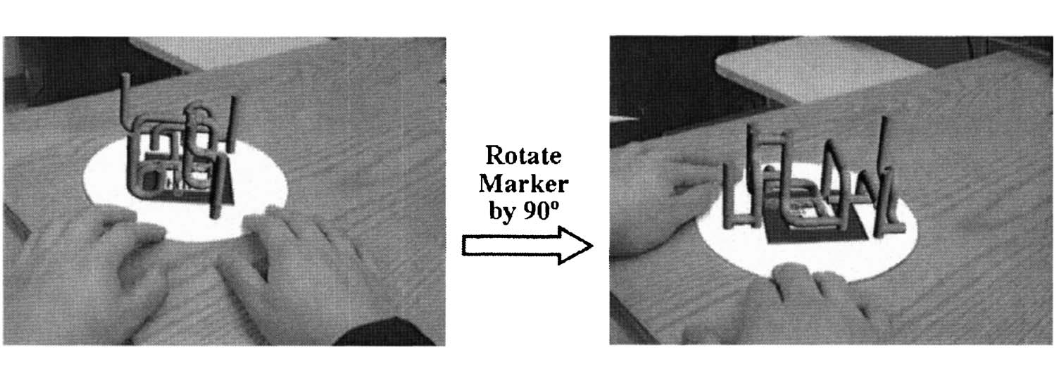
\includegraphics[width=0.97\textwidth]{img/rb-industry.png}
            \caption{\Wearable\ que permite a visualização e manuseio de projetos virtuais por meio de realidade aumentada. Fonte: \citet{dunston2005mixed}.}
            \label{fig:industry}
        \end{figure}
        
        % problemas
        \citet{patel2015wearable} aponta também quatro pontos que ainda representam problemas para o desenvolvimento e uso dos dispositivos \wearable\ e sua estabilização no cotidiano dos usuários.
        O primeiro é que uma pessoa deve ser motivada suficientemente para querer o dispositivo e estar disposta a utilizá-lo.
        Segundo, uma vez adquirido um dispositivo \wearable\ o usuário deve lembrar constantemente de utilizá-lo e ocasionalmente recarregá-lo.
        Terceiro empecilho é que a maioria dos dispositivos devem ser aptos a registrar de forma acurada os dados de seu ambiente utilizado sensores e aturadores.
        E por último, assumindo que a informação for lida com acurácia, os dados devem também serem apresentados ao usuários de forma compreensível para o seu entendimento das atividades realizadas e também motivando o uso contínuo do dispositivo.
        Dessa forma, mesmo que eles tenham grande potencial para facilitar a vida de usuários, a mudança não ocorre somente pelos dispositivos, necessitando uma grande demanda do hábito do usuário para seu uso.
        
        %cada vez mais usados
        Mas estudos como o de \citet{cornelius2014wearable} mostram que utilização de dispositivos eletrônicos inteligentes nas as redes de área corporal (do inglês \textit{body area network}) são cada vez mais usadas para monitoramento da saúde, assistência pessoal, entretenimento e automação residencial \citep{cornelius2014wearable}.
        
        
        % exemplo do crescimento 
        Um exemplo de seu potencial crescimento é no interesse cada vez mais de usuários tanto para uso quanto para desenvolvimento destes.
        \citet{merkouris2015introducing} em seu trabalho, avaliou experimentalmente a comparação dos benefícios da computação robótica e \wearable\ como plataforma meio no ensino de programação de dispositivos para crianças.
        Avaliaram atitudes e emoções dos estudantes antes e depois dos uso das plataformas de desenvolvimento e concluíram que utilizar computação obliqua como meio para aprendizagem de programação computadores é mais efetivo que o ensino de desenvolvimento para plataformas \textit{desktop} utilizadas geralmente.
        Citam também que mesmo que desenvolvimento para dispositivos \wearable\ não tenha sido tão motivador comparado com plataforma robótica, ainda sim apresentou-se mais interesse nas crianças que plataformas \textit{desktop}.
        
        
        % wearable e FPGA
        Além desses dispositivos, existe também desenvolvimentos de produtos \wearables\ que envolvem módulos em \hardware\ reconfiguráveis.
        Essa união permite que o \wearable\ utilize recursos de \hardware\ reconfigurável para suas tarefas além de poder se construído em totalmente nessa arquitetura sistêmica.
        O fruto deste produto entre essas tecnologias nos permite o alcançar maior poder de processamento com eficiência energética que processadores e microcontroladores tradicionais, desde que a aplicação corresponda bem às estruturas espaciais dos FPGAs \citep{Plessl2003}.
        \citet{demarco2011real} cita que enquanto adicionar a tecnologia de um FPGA em um projeto \wearable\ pode ter parecido complicado no \design,\ o FPGA fez com que fosse possível expandir facilmente as capacidades do sistema \wearable\ em momentos futuros.
        Um exemplo de conceito de uso é exibido na Figura~\ref{fig:rb-fpga} onde é descrito de forma esquemática um sistema para o monitoramento fetal domiciliar. 
        
        \begin{figure}[h] \centering
            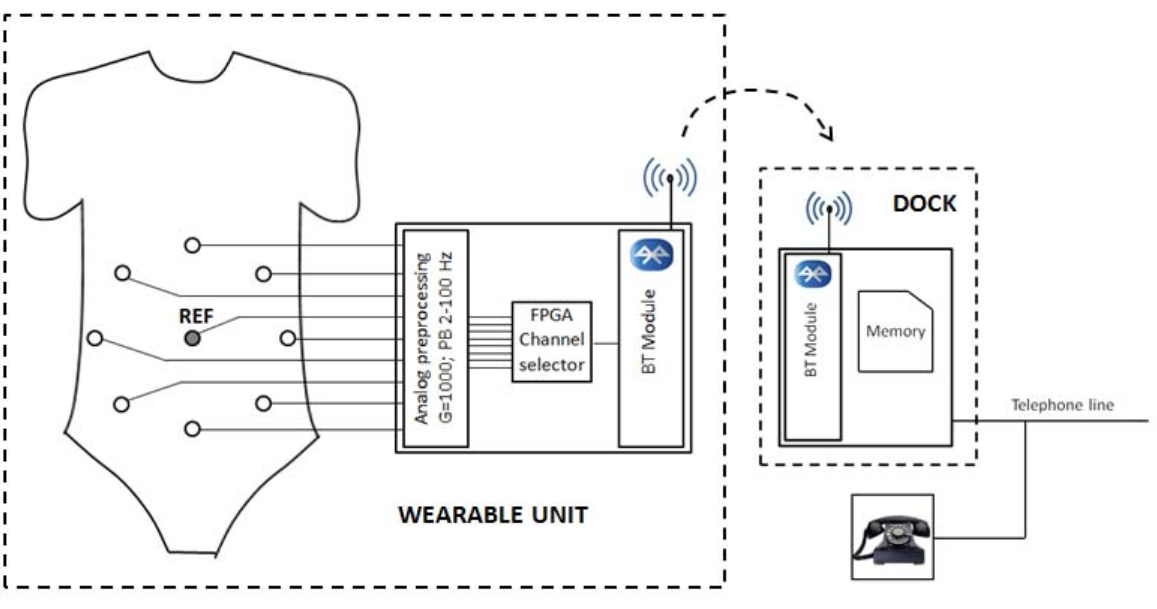
\includegraphics[width=0.97\textwidth]{img/rb-fpga.png}
            \caption{Monitoramento fetal domiciliar utilizando um FPGA e comunicação sem-fio. Fonte: \citet{fanelli2010prototype}.}
            \label{fig:rb-fpga}
        \end{figure}
        
        Caracteriza-se por uma unidade \wearable\ e uma estação de \textit{dock}. 
        Este é composto por um gravador colocado no na região do umbigo. 
        Um primeiro estágio opera um pré-processamento analógico com um FPGA extraindo a série, selecionando o canal com o melhor conteúdo de informação e os envia para o \textit{dock} através de uma conexão Bluetooth. 
        O \textit{dock} armazena as gravações em uma memória e as envia para o hospital através da linha telefônica.
        
        
        
	% !TeX spellcheck = pt_BR
%!TEX root = ../main_text.tex
\chapter{Trabalhos Relacionados} \label{chap:relacionados}

    \begin{comment}
    
    %not embedded
    O particionamento de forma geral é um problema de otimização na qual vários autores utilizam métodos para auxiliar na decisão de cada componente do \design\ referencial de \software. 
    Utiliza-se tanto processos manuais quanto algoritmos exatos ou heurísticos \citep{Arato2005}.
    
    \begin{wrapfigure}{r}{0.4\textwidth} \centering
        \vspace{-20pt}
        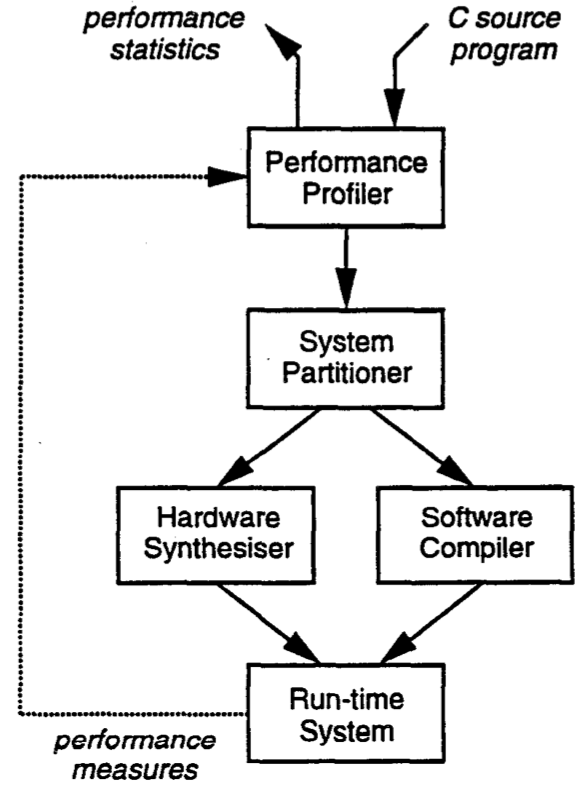
\includegraphics[width=0.4\textwidth]{img/rt-edwards_method.png}
        \vspace{-10pt}
        \caption{Metodologia de \codesign. Fonte: \citet{Edwards1994}.}
        \label{fig:tr-edwards_method}
    \end{wrapfigure}
    
    Os autores \citet{Edwards1994} utilizam do particionamento para aprimorar o desempenho do seu \software. 
    Em seu trabalho, realiza-se a tentativa de tratar regiões críticas da aplicação na qual uma solução em \software\ não pode chegar à restrições de desempenho requeridas e uma solução em \hardware\ deve ser encontrada, ou o desempenho total pode ser acelerada pela implementação de uma região crítica em \hardware.
    Apresenta-se uma metodologia para desenvolvimento \codesign\ no qual consiste na construção do código de uma aplicação em \textit{C} e as regiões críticas são identificadas e particionadas. 
    Feito isso realizar-se mensurações do projeto e uma nova verificação de particionamento é realizada, como é exibido na Figura \ref{fig:tr-edwards_method}.
    Utiliza-se também de um FPGA para as mensuras de desempenho e a propriedade de reconfiguração para novos testes em \hardware.
    
    Já o trabalho de \citet{Stitt2003} procura uma abordagem utilizando métodos de otimização de \software\ dinâmicos, introduzindo a primeira abordagem para particionamento de \hs\ dinâmico.
    O processo consiste na detecção da região de \software\ mais frequentemente executada e reimplementa-a em \hardware\ de FPGA.
    Afirmam que a utilização de particionamento dinâmico trás uma série de vantagens comparado com abordagens tradicionais manuais.
    
    Existem vários trabalhos que propuseram algoritmos exatos baseados em estratégias \textit{branch-and-Bound} \citep{Jigang2004, Mann2007, Strachacki2008}, programação dinâmica \citep{Madsen1997, Wu2006} e linear inteira (ILP, do inglês \textit{integer linear programming}) \citep{Niemann1997}.
    
    \citet{Nematbakhsh_theeffect} parte para o exame da relação entre o \textit{footprint} gerado para o FPGA e o \speedup\ do \software\ na situação na qual um FPGA é utilizado para a implementação de \textit{loops} e sub-rotinas críticas.
    Como utilizam uma abordagem direta, utilizaram de ferramentas protótipos e comerciais como \textit{Synopys' Nimble Compiler} e \textit{Proceler}, para a facilitação do processo.
    
    Abordagens mais recentes como a de \citet{Yan2017} parte da otimização \textit{position disturbed particle swarm} com otimização invasiva de \textit{weed} como o método de particionamento \hs.
    
    \citet{Wang2016} citam que o particionamento depende da exploração de caracterização, estimação e \design\ espacial das métricas de custo e desempenho sistêmico. 
    É também mencionado que o \codesign\ nos dias de hoje é tão complexo que a simplificação do particionamento só para duas partes não é suficiente para a representação do problema como um todo. 
    Sobre essa crítica, dissertam sobre a inclusão de parâmetros chave de \design\ e uso de recursos que deveriam ser incorporados à modelagem do sistema e dessa forma, o trabalho proposto visa considerar a modelagem de incerteza para particionamento de sistemas com um conjunto melhorado de parâmetros para compartilhamento de recursos \hs.
    Esse terceiro item a ser considerado ao problema de particionamento podem ser definidos em três tipos, sendo esses: 
    \textit{a)} o conjunto de recursos necessários para particionar uma dada tarefa (sendo esses RAM, ROM, DPS, blocos IP do inglês, \textit{intelectual propriety}, entre outros); 
    \textit{b)} possuem vários parâmetros de configurações que provê diferentes \textit{trade-off} entre recursos e desempenhos como por exemplo circuitos de multiplicações/divisões que podem ser sintetizados sequencialmente (pouca área e lento) ou combinatório\footnote{Por \textit{unrolling}, técnica de otimização de código no qual tenta reduzir ou eliminar as iterações de determinado \textit{loop} do código.} (muita área e rápido); 
    \textit{c)} a dificuldade da mensura de desempenho e impacto no uso de recursos em várias configurações de partição com precisão precisando ter em mente a partição com a natureza incerta dessas estimativas não precisas.
    A teoria da incerteza é uma abordagem que é um sistema matemático que é designado para modelar a indeterminação ao invés do uso da teoria da probabilidade. 
    Isso pois, quanto tem-se muitas amostras de uma quantidade indeterminada, seria significativo a utilização da teoria de probabilidade ou \textit{fuzzy} pela propriedade de serem contínuas entre o intervalo 0 (zero) à 1 (um). 
    Entretanto, se não possui-se amostras suficientes para a estimação de uma distribuição de probabilidade, utiliza-se do conhecimento do domínio para avaliação do grau de crença de que cada evento indeterminado acontecerá, no caso, aplicado pela teoria da incerteza. 
    E a teoria da incerteza é um ramo da matemática axiomática para modelagem de graus de crença, de modo geral.
    
    Como outro trabalho recente que aborda o particionamento, \cite{Choi2016} descreve um \textit{framework} chamado LegUp.
    Com essa ferramenta é possível compilar um \software\ e suas \textit{threads} gerando um sistema \textit{hardware-only} ou também um sistema híbrido particionado paralelo utilizando aceleradores, gerando também todos os itens necessários para tal como memórias sintetizadas e sistemas de interconexões.
    Utilizam duas técnicas de descrição de paralelismo em \software\ sendo elas a \textit{Pthreads} e a \textit{OpenMP} sendo a primeira permite a sintetização de funções operando concorrentemente em \hardware\ com aceleradores, e a segunda usada para gerar os próprios aceleradores executados concorrentemente em um sistema de compartilhamento de memória.
    Afirmam também que a sua ferramenta produz HDL de alto desempenho que pode ser comparado com circuitos que são gerados por ferramentas HLS comerciais. 
    Os resultados obtidos pelos cientistas \cite{Canis2011} mostraram que a ferramenta consegue gerar produtos tão bons quantos ferramentas HLS comerciais.
    
    Entretanto, além de todo arcabouço de algoritmos para escolhas para sistemas de propósito geral tal como os citados, existe ainda uma linha de pesquisa específica do problema na qual trata-se do particionamento em sistemas embarcados.
\end{comment}
    
    % Embedded
    % optimization problem
    A busca por otimização em dispositivos gerais com foco no problema de particionamento \hs\ já é amplamente pesquisado como é exibido nos trabalhos de \citet{Ernst1993, Gupta1995, Hardt1995, Gajski1994, Bolsens1997}, publicados na década de 90.
    
    \citet{Mei2000} descrevem um particionamento de \hs\ além de uma abordagem de escalonamento para Sistemas Embarcado Dinamicamente Reconfiguráveis (DRESs, do inglês \textit{Dynamically Reconfigurable Embedded Systems}) na qual possuem como projeto um processador de propósito geral junto com um FPGA sendo este reconfigurável em tempo de execução para reduzir custos.
    Dessa forma, analisaram o tempo de configuração e, como contribuição, a análise do tempo de reconfiguração parcial do FPGA.
    %Com a adição da reconfiguração parcial de \hardware, o escalonamento no FPGA torna-se um problema de alocação restrita, enquanto o escalonamento em circuitos integrados de aplicação específica (ASICs, do inglês \textit{application-specific integrated circuits}) é um problema de serialização.
    Para o escalonamento, utilizam um método baseado na heurística do Algoritmo Genético (GA, do inglês \textit{Genetic Algorithm}) e num algoritmo de escalonamento de lista com melhorias.
    O escalonador desenvolvido atua como uma sub-rotina do algoritmo de particionamento. 
    Ele é invocado no passo de evolução da população do GA. 
    Além do escalonamento já conhecido que determinam a ordem e tempo de execução, o algoritmo também faz o escalonamento no FPGA não só determinando o tempo de início da tarefa, mas sim sua posição no FPGA respeitando as restrições de recursos e precedentes, tornando assim o problema uma abordagem ao problema de alocação restrita.
    
    \citet{Arato2003} descrevem algumas versões diferentes do problema de particionamento, correspondendo à sistemas de tempo-real e custo restringido respectivamente, fornecendo análise matemática formal para os problemas, provando que são problemas $ \mathcal{NP} $-difíceis. 
    Apresentam uma abordagem baseada na Programação Linear Inteira (ILP, do inglês \textit{Integer Linear Programmimg}) resolvendo o problema de particionamento forma otimizada mesmo para sistemas de grande porte, além de outra abordagem utilizando a heurística de GA na qual encontram soluções próximas ao ótimo global para sistemas largos.
    Este problema representa um subgrupo da programação linear no qual algumas ou todas as variáveis do problema pertencem ao conjunto dos números inteiros. A tentativa de solucionar um PLI para um modelo puro com quantidades de restrições é um problema $\mathcal{NP}$-difícil.
    
    
    \citet{Mann2007} descrevem uma primeira tentativa para um algoritmo exato, não heurístico, do problema. 
    Utilizam um esquema na qual implementa-se a estratégia \textit{branch-and-bound} como um arcabouço, permitindo o incremento de outros algoritmos de forma complementar. 
    Em sua implementação, realizaram várias investigações para incrementar a eficiência do algoritmo, incluindo várias técnicas como: \textit{lower bounds based on LP-relaxation}, mecânica de inferência customizada, condições não-triviais necessárias baseadas num algoritmo \textit{minimum-cut} e diferentes heurísticas com passos pré-otimizados. 
    O algoritmo pode incluir mais de uma restrição, permitindo o \designer\ prescreva quais nós devem estar em qual nível no \design. 
    Eles demonstram que o produto final pode resolver problemas de particionamento altamente complexos em tempo razoável. 
    Citam que o resultado obtido é em entorno de dez minutos mais rápido que algoritmos exatos anteriores baseados em ILP para os testes realizados.
    
    Pesquisas mais recentes como a de \citet{BenHajHassine2017} procuram aplicar otimizações sobre o tempo de execução e gasto energético para \cores\ de SE por meio de particionamento.
    O algoritmo proposto destina-se alcançar um particionamento de grafos à procurar o melhor conjunto da relação energia e tempo de execução.
    Testado em comparação com outros algoritmos heurísticos como \textit{Simulated Annealing}, Busca Tabu e GA, mostrou-se ser mais adequado para tais aplicações.
    
    \citet{Trindade2016} utiliza do GA para solucionar o problema de particionamento em sistemas embarcados. 
    Propõe-se novas abordagens para o problema usando técnicas de verificação baseadas nas Teorias de Módulo de Satisfabilidade (SMT, do inglês \textit{Satisfiability Modulo Theories}). 
    Apresentam um exemplo, modelam e solucionam-o usando três diferentes técnicas sendo a principal ideia é aplicar o método de verificação SMT ao particionamento \hs, e por fim, comparam os resultados com técnicas de otimizações tradicionais como ILP e GA.
    
    
    
    Os trabalhos descritos acima buscam o estudo do desempenho e \design\ de SE no geral por meio de otimizações sobre o problema de particionamento em sistemas embarcados, mas nenhum abordando sistemas \wearables.
    
    
    
    
    \citeauthor{Jozwiak2017} em seu \textit{survey} publicado em \citeyear{Jozwiak2017}, apresenta uma extensa revisão da literatura considerando vários aspectos de um SE, bem como suas tecnologias de \design\ com foco em sistemas modernos incluindo \wearables.
    Cita-se dois paradigmas de desenvolvimento para SEs sendo eles o paradigma de sistemas \textit{life-inspired} e sistemas \textit{quality-driven}.
    O paradigma de sistemas \textit{life-inspired} especifica princípios básicos, características e organização funcional e estrutural de um SE por meio da analogia à vida de um organismo inteligente, além de básicas soluções de mecanismos e arquiteturas de sistemas para implementar tais princípios. 
    Já o paradigma de sistemas \textit{quality-driven} ou seja, orientado pela qualidade, caracteriza dispositivos que necessitam satisfazer as exigências de \textit{real-time}, baixo consumo de energia, entre outros. 
    %
    %Dessa forma, especifica-se qual a nova qualidade do sistema a ser requeria e como esta meta é obtida. 
    Ainda define qualidade de uma solução sistêmica proposta como o total de sua eficácia e eficiência na resolução do problema real. 
    %Eficácia entende-se como o grau em que uma solução atinge seus objetivos e a eficiência o grau em que uma solução usa recursos para realizar seus objetivos e juntas determinam o grau de excelência. 
    Elas são expressas em termos de parâmetros mensuráveis, o que é necessário para implementar o design \textit{quality-driven}.
    %Entretanto, é descrito ao final que, enquanto \designers\ aprenderam bastante na construção de plataformas de \hardware\ heterogêneos altamente paralelos, os métodos e ferramentas automatizadas para a sua programação e o paralelismo do algoritmo, bem como o \codesign\ coerente da arquitetura \hs\ ainda são atrasados perante à tecnologia.
    Além deste é possível ver documentos de \citet{Plessl2003, Ahola2007, Abdelhedi2016, Narumi2016, Lee2015} sobre \wearables\ junto de FPGA, mas nenhum utilizando a técnica de particionamento como meio para seu \design.
    
    
    
    Este trabalho portanto consiste na análise do problema de particionamento \hs,\  com foco em \design\ de sistemas \wearables\ em plataforma FPGA.
    
    
    \section{Comparativo entre os Trabalhos}      
        
        Fazendo uma relação entre a pesquisa proposta com os trabalhos relacionados, é possível visualizar pela Tabela~\ref{tab:comparativo_trabalhos} que, este trabalho propõe uma abordagem de particionamento \hs\ para \design\ de sistema \wearable\ em \hardware\ reconfigurável a fim de buscar otimizações em seu desempenho utilizando recursos em \hardware.
        
        \begin{table}[h] \scriptsize
            \caption{Comparativo visual entre os principais itens tratado nos trabalhos citados e o trabalho apresentado.}
            \label{tab:comparativo_trabalhos}
            \rowcolors{1}{lightgray}{white}
            \begin{tabularx}{\textwidth}{|X|c|c|c|X|} \hline
                \textbf{Trabalhos Relacionados} \centering & 
                                         \specialcell{\textbf{Particio-}\\\textbf{namento}} &
                                                  {\textbf{SE/}\textbf{\Wearable}} & 
                                                                     \textbf{FPGA} & 
                                                                              \textbf{Observações Adicionais} \\ \hline \hline
                
%                \citet{Edwards1994}           & \cmark & \cmark\ / \xmark & \cmark & Proposta de uma metodologia nova \\ \hline
%                \citet{Stitt2003}             & \cmark & \cmark\ / \xmark & \cmark & Particionamento Dinâmico \\ \hline
%                \citet{Jigang2004, Mann2007, 
%                Strachacki2008}               & \cmark & \xmark\ / \xmark & \xmark & \textit{Branch-and-bound} \\ \hline
%                \citet{Madsen1997, Wu2006}    & \cmark & \xmark\ / \xmark & \xmark & Prog. dinâmica \\ \hline
%                \citet{Niemann1997}           & \cmark & \xmark\ / \xmark & \xmark & Prog. linear inteira \\ \hline
%                \citet{Nematbakhsh_theeffect} & \cmark & \xmark\ / \xmark & \cmark & \textit{Footprint} FPGA vs. \speedup\ \software \\ \hline
%                \citet{Yan2017}               & \cmark & \xmark\ / \xmark & \xmark & Otimização \textit{position disturbed particle swarm} \\ \hline
%                \citet{Wang2016}              & \cmark & \cmark\ / \xmark & \cmark & Modelagem de incerteza para o particionamento \\ \hline
%                \citet{Choi2016}               & \cmark & \xmark\ / \xmark & \cmark & \textit{Framework} LegUp \\ \hline
                
                % embedded
                \citet{Mei2000}               & \cmark & \cmark\ / \xmark & \cmark & Processador (Particionamento e escalonamento para sistemas embarcados dinamicamente reconfiguráveis com GA) \\ \hline
                \citet{Arato2003}             & \cmark & \cmark\ / \xmark & \xmark & Particionamento para RTOS e custo restringido, utiliza-se de prog. linear inteira \\ \hline
                \citet{Mann2007}              & \cmark & \cmark\ / \xmark & \xmark & \textit{Branch-and-bound} \\ \hline
                \citet{BenHajHassine2017}           & \cmark & \cmark\ / \xmark & \xmark & Otimizações em \cores. Particionamento que visa o tempo de execução vs. gasto energético \\ \hline
                \citet{Trindade2016}          & \cmark & \cmark\ / \xmark & \xmark & Utiliza algoritmo genético \\ \hline
                \citet{Jozwiak2017}           & \cmark & \cmark\ / \xmark & \xmark & \textit{Survey} sobre particionamentos em sistemas embarcados. Classifica-os em dois paradigmas: \textit{life-inspired} \textit{quality-driven} \\ \hline
                % fpga
                \citet{Plessl2003, Ahola2007, 
                Abdelhedi2016, Narumi2016, 
                Lee2015}                      & \xmark & \cmark\ / \cmark & \cmark & Não realizam análise metodológica sobre o problema de particionamento \\  \hline \hline
                \textbf{Trabalho Proposto}    & \cmark & \cmark\ / \cmark & \cmark & \textbf{Análise em \wearable\ com foco em aumento de desempenho e controle energético e recursos} \\ \hline
            \end{tabularx}
        \end{table}

    A tabela exibe todos os trabalhos apresentados de forma a pontuar as ferramentas e os propósitos.
    Como existe muitos trabalhos que abordam SE, foi adicionado uma especificação indicando se além do foco em SE o trabalho aborda uma análise em sistemas \wearables.
    Da mesma forma, há trabalhos que trabalham com o particionamento \hs\ mas sem foco em \wearables, outros que não utilizam de plataformas FPGA como meio e outros que trabalham com \wearables\ e FPGA mas o objetivo do estudo do particionamento.
    Assim, a pesquisa tende realizar uma análise utilizando todos estes conceitos, sendo eles, o particionamento para \wearables\ utilizando plataformas FPGAs na obtenção de desempenho e gasto energético consciente.
    
    
    A seguir, serão apresentados os tópicos são necessários para o entendimento básico dos arcabouços metodológicos de \codesign\ e o seu particionamento para sistemas embarcados, em especial para sistemas \wearable, além de definições matemáticas sobre.
	%!TEX root = ../main_text.tex
\chapter{\Design\ de Sistemas \Wearable} \label{chap:design}

   A seguir, serão descritos alguns tópicos seguindo conceitos estabelecidos pelo livro de \citet{Sass2010} e utilizado por vários trabalhos como \citet{Arato2003, Arato2005, Mann2007, Hassine2017}.
   %Esses tópicos são necessários para o entendimento básico dos arcabouços metodológicos de \codesign\ e o seu particionamento para sistemas embarcados, em especial para sistemas \wearable, além de definições matemáticas sobre.

   Os tópicos a seguir são a Definição de \Design\ de Referência de \Software\ (Seção~\ref{sec:GCF}) bem como o Ganho de Performance (Seção~\ref{sec:ganho_performance}) em tais sistemas, o Particionamento \HS\ para Sistemas \Wearables\  (Seção~\ref{sec:desenvolvimento}) e a Proposta de Procedimento Analítico (Seção~\ref{sec:proposta}).

   \section{Introdução ao \Design\ Referencial de \Software\ Utilizando Grafo de Controle de Fluxo} \label{sec:GCF}

      \begin{wrapfigure}{O}{0.4\textwidth}
      	\centering
      	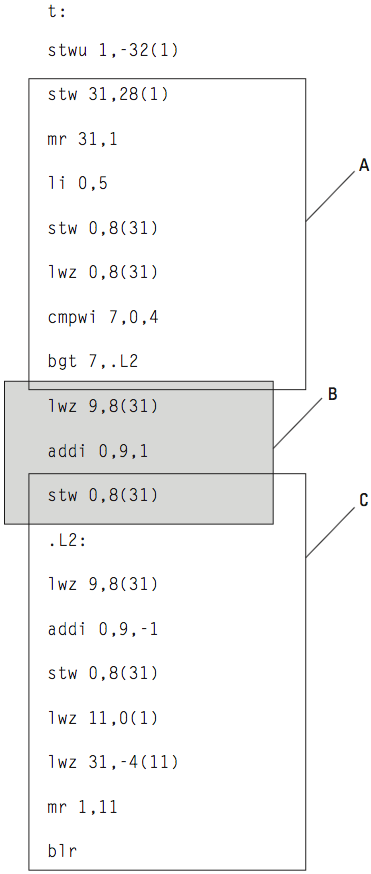
\includegraphics[width=0.35\textwidth]{img/f3-5.png}
      	%\vspace{10pt}
      	\caption{Identificação de blocos básicos em um código \assembly.}
      	\label{fig:blocos_basicos}
      	%\vspace{-15pt}
      \end{wrapfigure}

      É possível descrever sistemas livre de especificações formais de \software\ ou \hardware\ por meio de descrições de protótipos simples.
      Estes, conhecidos como \design\ referencial de \software.
      Como será visualizado a seguir, sua vantagem mais notável é a generalização de uma especificação completa, eliminando quaisquer tipo de incertezas sobre o comportamento do sistema ao realizar uma análise sobre, sendo este podendo ser representado por diversas formas.
      % além de outras como o fato de que sua especificação pode ser analisada por ferramentas computacionais, e gerando modelos aut.

      %Assumindo que o \design\ de referência de \textit{software} já exista,
      %Primeiramente, será demonstrado matematicamente como computação está em \design\ referencial de \sof%htware\ para que depois, isso possa nos auxiliar na decisão do que deverá ser implementado em nível de \hs.
      Como o algoritmo a ser analisado e particionado também pode ser representado em forma de grafo de tarefas/rotinas, pode-se então associar o \design\ da sub-rotina também com o uso da teoria de grafos \citep{Mann2007}, em especial o Gráfico de Controle de Fluxo (GCF).
      Ele é definido por
      \begin{equation}
         C = (B, F) \label{eq:subrotina}
      \end{equation}

       onde $B$ são vértices que representam os blocos básicos\footnote{De modo geral é um trecho de código sequencial maximal, onde só existe um ponto de entrada e um ponto de saída.}
      %http://www.dcc.ufrj.br/~gabriel/microarq/Escalonamento.pdf
      e $ F $ são arestas que indicam a todas as possibilidades de caminhos entre os blocos.

      Utilizando o exemplo da Figura \ref{fig:blocos_basicos}, o primeiro grupo \A\ é um bloco não básico porque não é maximal, ou seja, a primeira instrução \texttt{store word with update} deveria estar incluída ao grupo para conter o número máximo de instruções possuindo apenas um ponto de entrada e saída.
      Grupo \B\ é um bloco básico e o grupo \C\ não se define como bloco básico pois existe duas entradas para o bloco, sendo elas na instrução \texttt{store word} e também pelo \texttt{branching} direcionado para \texttt{L2}.

      Dessa forma, fazendo uma relação entre o processo de gerar um grafo de controle de fluxo a partir de um código em alto nível, a Figura~\ref{fig:f3-6} exibe um pequeno código demonstrativo na qual o processo ocorrerá.
      A partir do código em alto nível (Figura~\ref{fig:f3-6} \textit{a)}) é identificado os blocos básicos de acordo com o compilador\footnote{Deve-se atentar que, só é possível identificar blocos básicos em um arquivo em linguagem de programação \textit{C} desde que se saiba qual compilador foi utilizado para emitir o código \assembly.} utilizado.
      Neste exemplo, utilizou-se de um compilador para \texttt{PowerPC}\footnote{Arquitetura que utiliza RISC como arquitetura do conjunto de instruções.} onde os blocos básicos são identificados pela Figura~\ref{fig:f3-6} \textit{b)}.
      Por fim o grafo de controle de fluxo resultante deste processo, representado pela Figura~\ref{fig:f3-6} \textit{c)}.

      \begin{figure}[h] \centering
         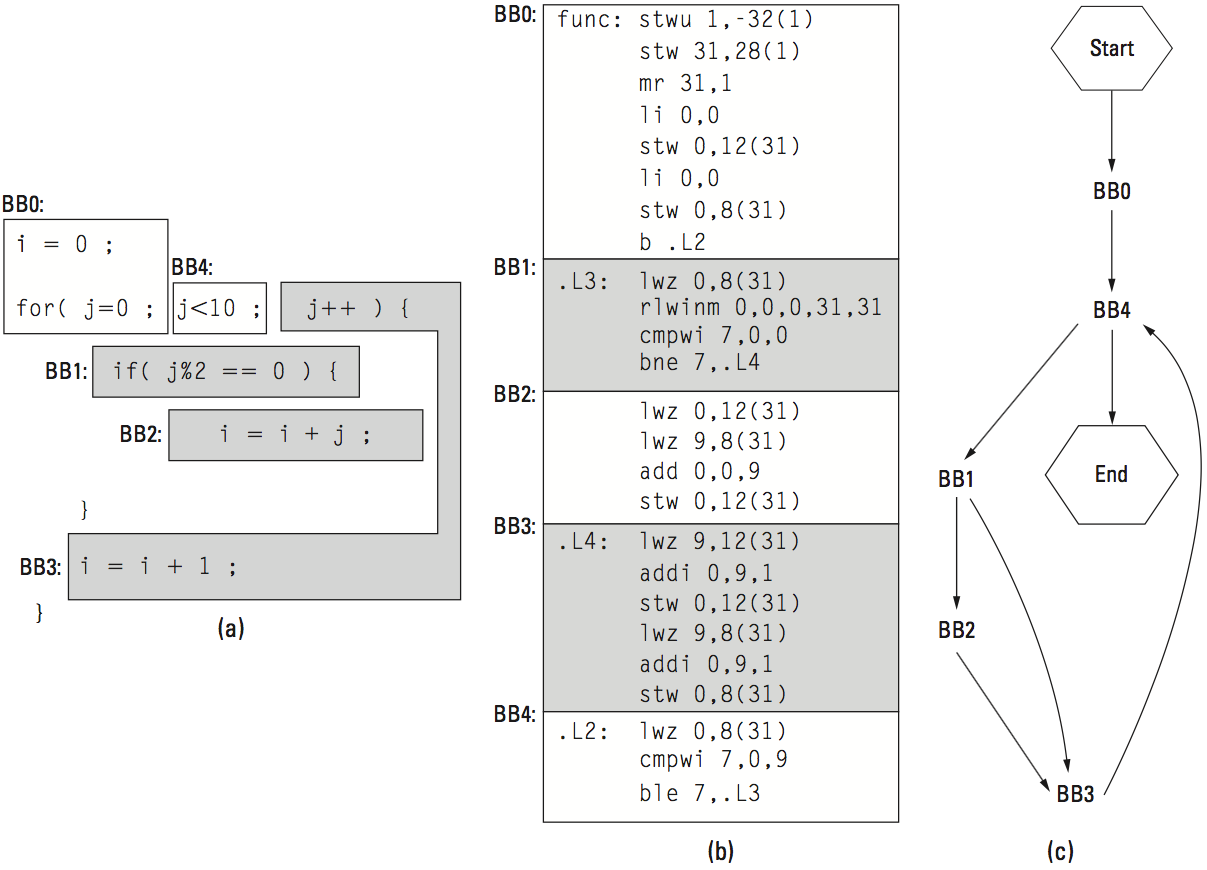
\includegraphics[width=0.95\textwidth]{img/f3-6.png}
         \caption{Identificação de blocos básicos e a representação por meio de um grafo não atrelado à uma especificação \hs.}
         \label{fig:f3-6}
      \end{figure}

      A decomposição de um \design\ referencial de \software\ pode gerar dois componentes: uma porção a ser realizada em \hardware\ e; outra executada em \software.
      Essa decisão de divisão é chamada de Problema de Particionamento.
      Segundo \citeauthor{Sass2010}, para sistemas em FPGA, o particionamento é um sub-problema de um problema mais geral no âmbito de \codesign, onde refere-se ao \design\ cooperativo entre engenheiros de \hs\ para um desenvolvimento mais eficiente.% envolvendo \textit{stakeholders}, por exemplo.
      %Para continuar, deve-se definir alguns conceitos básicos, descritos na Seção \ref{sec:gc}.

      \subsection{Grafo de Chamada} \label{sec:gc}
         Modelado uma sub-rotina de um \design\ referencial de \software\ utilizando o grafo de controle de fluxo, definido na Seção \ref{sec:GCF}, agora será descrito uma nova notação, chamada de Grafo de Chamada (GC) utilizado para o entendimento da partição.
         Consiste num conjunto de GCFs, um por sub-rotinas, ou seja,
         %
         \begin{equation}
            \mathcal{C} = {C_0, C_1, \dots C_{n-1}}
         \end{equation}
         %
         %onde $ C_i = (V_i, E_i) $
         onde $ C_i = (B_i, F_i) $ representa o grafo de controle de fluxo de uma sub-rotina $ i $, como mostrado na Equação~\ref{eq:subrotina}.
         Sendo assim, o grafo estático de chamada da aplicação é escrito por
         %
         \begin{equation}
            \mathcal{A} = (\mathcal{C}, \mathcal{L}) \label{eq:a}
         \end{equation}
         %
         onde \A\ representa uma aplicação específica e $ \mathcal{L} \subseteq \mathcal{C} \times \mathcal{C} $ é um subconjunto do plano cartesiano dos GCF.
         Duas sub-rotinas são relacionadas se podem ser determinadas que, no tempo de compilação, a sub-rotina $ i $ tem potencial de invocar a sub-rotina $ j $, ou seja, $ (C_i, C_j) \in \mathcal{L} $.

         É assumido que os blocos básicos de cada sub-rotina são disjuntos, ou seja, cada bloco básico em uma aplicação pertence a exatamente um GCF.
         Além do mais, é assumido também que um nó raiz para o GC é implícito, ou seja, uma sub-rotina é designada a iniciar a execução.
         Nem todos os executáveis podem ser expressados nesse modelo.
         Por exemplo, o manuseio de sinais e interrupções não são representadas e assim, não é possível determinar todos vértices $ F_i $ em uma dada sub-rotina $ C_i $ de um GCF antes da execução.
         %Uma outra forma é com o paradigma de orientação à objeto.
         %Ele depende do tempo de execução para conectar os métodos virtuais invocados e dessa forma, por \design, esse paradigma nos previne de saber todos os vértices antes da execução.
         %Para agora, será considerado que o modelo é suficiente para ser expressado em \design\ referencial de \software.

         Um equívoco comum é de que uma definição formal de particionamento só aplica à separação de aplicação componentes de \hs, ou seja, a partição contém exatamente dois conjuntos.
         Todavia, para fazer o problema mais tratável, é comum agrupar primeiramente operandos em recursos, ou seja, uma partição com um grande número de subconjuntos, e então mapeia esses recursos tanto em \hardware\ quanto \software.
         Assumindo que esses recursos atuam razoavelmente bem \textit{clustered}, então a decomposição de uma aplicação em componentes de \hs\ pode ser dirigida por comparações de ganho de performance desse recurso contra outro situado no outro conjunto.

         Definidos os conceitos prévios, será definido agora, formalmente, o conceito de uma partição.

         Uma partição $ \mathcal{S} = \{S_0, S_1, \dots\} $ de um conjunto universal $ U $ é um conjunto de subconjuntos de $ U $ sendo que
         %
         \begin{equation}
            \bigcup_{S \in \mathcal{S}} S = U \label{eq:part_form_1}
         \end{equation}
         \begin{equation}
            \forall S, S' \in \mathcal{S} | S \cap S' = \emptyset \label{eq:part_form_2}
         \end{equation}
         e assim
         \begin{equation}
            \forall S \in \mathcal{S} \cdot S \neq \emptyset \label{eq:part_form_3}
         \end{equation}
         %
         Descrevendo textualmente:
         \begin{description}
            \item [Equação \ref{eq:part_form_1}:] cada elemento de $ U $ é um membro de, pelo menos, um subconjunto $ S \in \mathcal{S} $;        

            \item [Equações \ref{eq:part_form_2} e \ref{eq:part_form_3}:] os subconjuntos $ S \in \mathcal{S} $ são emparelhados disjuntos e não vazio.
            Em outras palavras, cada elemento do nosso universo $ U $ termina exatamente em um dos subconjuntos de $\mathcal{S}$ e nenhum dos subconjuntos são vazios.

         \end{description}

         %exemplo
         Por exemplo, considerando um sistema hipotético \wearable\ na qual possui o universo $ U = \{a, e, i, o, u, y\} $ de recursos de processamento.
         Dessa forma, uma partição desse problema $ \mathcal{X}_a $ de $ U $ pode ser representado por
         %
         \begin{equation}
         \mathcal{X}_a = \left\{\{a, e, i, o, u\}, \{y\}\right\} \label{eq:xa}
         \end{equation}
         %
         e supondo que o conjunto possa ser representando por cada unidade, uma outra forma de representação pode ser
         %
         \begin{eqnarray}
         \mathcal{X}_b &=& \left\{\{a\}, \{e\}, \{i\}, \{o\}, \{u\}, \{y\}\right\} \label{eq:part_a} \\
         \mathcal{X}_c &=& \left\{\{a\}, \{e\}, \{i\}, \{o\} \right\} \label{eq:part_c} \\
         \mathcal{X}_d &=& \left\{\{a, e, i\}, \{i, o, u, y\}, \{\}\right\} \label{eq:part_d}
         \end{eqnarray}
         %
         Sobre tais conceitos, a Partição \ref{eq:part_c} viola a Equação \ref{eq:part_form_1} e a Partição \ref{eq:part_d} viola as Equações \ref{eq:part_form_2} e \ref{eq:part_form_3}, pois a primeira omite um item $y$ e a segunda possui um conjunto vazio além de redundância.
         %
         Assim, ao utilizar o particionamento para este exemplo, a Figura \ref{fig:parti_alfabeto} ilustra o $ \mathcal{X}_a $ (Equação \ref{eq:part_a}) graficamente, segundo a Partição \ref{eq:xa} como seria uma divisão entre \hs\ dos recursos listados.

         \begin{figure}[h] \centering
            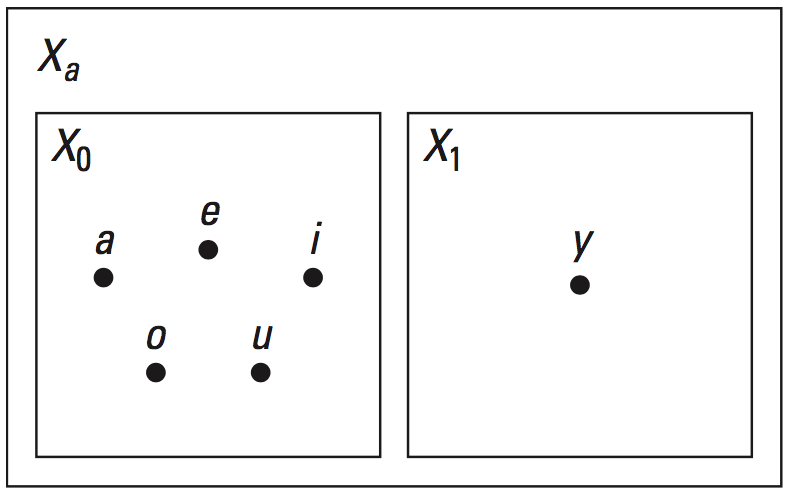
\includegraphics[width=0.5\textwidth]{img/f4-2.png}
            \caption{Figura representativa do mapeamento da aplicação.}
            \label{fig:parti_alfabeto}
         \end{figure}
%\end{commaent}

         Aprendido os conceitos, é possível aplicar o formalismo à $ \mathcal{A} $.
         Se assumirmos que nosso universo é o conjunto de todos os blocos básicos $B$ de todas as sub-rotinas de um dispositivo \wearable, então $U$ é as partições de sub-rotinas
         %
         \begin{equation}
            U = \bigcup_{C \in \mathcal{C}} B(C) \label{eq:bigcup}
         \end{equation}
         %
         e chamaremos de partição natural da aplicação, onde
         %
         \begin{equation}
            \mathcal{S}  = \left \{
            \underbrace{\left \{ b_0, b_1, \dots, b_i \right \}}_{\text{sub-rotina }C_0},
            \underbrace{\left \{ b_i, b_{i+1}, \dots, \right \}}_{\text{sub-rotina }C_1},\dots
            \underbrace{\left \{ b_j, b_{j+1}, \dots, \right \}}_{\text{sub-rotina }C_{n-1}}
            \right \}
         \end{equation}
         %
         O propósito é reorganizar a partição de blocos básicos e então mapear cada subconjunto de ambos os \hs.
         Dessa forma, estamos livres para criar e remover subconjuntos não vazios, e mover blocos básicos ao redor até termos uma nova partição e assim termos um novo resultado $ \mathcal{A}’ = (\mathcal{C}’, \mathcal{L}’) $, inferido a partir da reorganização da partição $ \mathcal{X}’ $.
         O segundo passo é mapear cada subconjunto de $ \mathcal{X} $ para ambos \hs\ como é exibido abaixo
         %
         \begin{equation}
            \mathcal{X}'   = \left \{
            \underbrace{
               \underbrace{
                  \left \{ b_j, b_{j+1}, \dots, \right \}
               }_{\text{sub-rotina }C_k}
               \underbrace{
                  \left \{ b_k, b_{k+1}, \dots, \right \}
               }_{\text{sub-rotina }C_l}
               \dots
            }_{\text{\software}}
            \
            \underbrace{
               \underbrace{
                  \left \{ b_0, b_1, \dots, b_i \right \}
               }_{\text{sub-rotina }C_r}
               \underbrace{
                  \left \{ b_i, b_{i+1}, \dots, \right \}
               }_{\text{sub-rotina }C_s}
               \dots
            }_{\text{\hardware}}
            \right \} \label{eq:part_final}
         \end{equation}


   \section{Ganho de Performance} \label{sec:ganho_performance}
      Para explicar como performance pode ser utilizada para guiar o particionamento, será descrita uma métrica simples chamada taxa de execução\footnote{Taxa de execução é a velocidade na qual um sistema computacional completa uma aplicação, e em um sistema de plataforma FPGA olhamos também para o \hardware\ para melhorar sua taxa de execução.}.
      É parcialmente motivada pelo fato de que: \textit{a)} o ganho de performance é relativamente fácil de ser mensurado e \textit{b)} por causa de que, de todas as métricas comumente utilizadas, \speedup\ é frequentemente a mais importante.
      Diferente do mundo \software\ onde se tem análise de ordem de complexidade, em \hardware\ não possui-se um guia geral para comparação.
      O ganho de performance para aplicações em geral pode estar na acumulação de pequenos ganhos que deveriam ser perdido numa aplicação direta na teoria de complexidade.

      % tempo software
      Assim, para o \software, será usado a informação de \profile\ (Seção \ref{sec:profile}) para coletar o tempo total de execução, bem com uma fração do tempo gasto em cada sub-rotina.
      O produto disso é a aproximação entre o tempo necessário para executar uma porção de aplicação em \software\ e usar isso como o tempo que se espera que tomará em futuras execuções.
      É considerado uma aproximação pois é dependente dos conjuntos de dados de entrada para muitas aplicações além da existência de erros que podem impactar a performance.
      Será utilizado $ s(i) $ para representar o tempo de execução esperado para uma invocação de uma sub-rotina $ i $, ou seja, bloco básico.

      % tempo hardware
      Precisa-se também aproximar o tempo que uma implementação equivalente em \hardware\ que iria tomar.
      No caso dos blocos básicos implementados, isso é frequentemente mais preciso.
      Como não possui-se um controle de fluxo, uma ferramenta auxiliar à síntese poderá dar uma aproximação de acurácia de propagação de tempo.
      Ou, se o recurso é \textit{pipelined}, o número de estágios é mais precisamente conhecido.
      Caso o recurso inclua controle de fluxo mas não contenha nenhum \textit{loop}, pode-se considerar o caminho mais longo como uma estimativa conservativa.

      Recursos com um número variável de iterações através de um \textit{loop} apresentam o maior obstáculo para encontrar um tempo de \hardware\ aproximado.
      Nesse caso, implementação e \textit{profiling} com recurso em \hardware\ pode ser a única solução.
      Independente, assume-se que uma aproximação apropriada $ h(i) $ para o existente tempo de execução em \hardware.

      % tempo mudanca de estado, configuracao, latencia
      Por fim, a `interfaceação' entre \hs\ requer tempo e este custo também precisa ser contabilizado.
      Pode-se aproximar deste custo pela aproximação do montante total do estado que necessita ser transferido ou o custo de configuração e latência.
      Em ambos os caso, são representados por $ m(i) $ para recursos $ i \in \mathcal{H} $, sendo $\mathcal{H}$ o conjunto de recursos do \hardware.

      % y é speedup
      O ganho, ao comparar uma solução \hs\ contra uma solução puramente \software, é tipicamente mensurado como \speedup.
      Utilizamos $ \gamma $ para sua representação e isso nos permitirá comparar recursos diferentes contra outros para determinar melhores particionamentos.
      Dessa forma, qualquer subconjunto de blocos básicos que não produzem um ganho de performance, podem ser excluídos de consideração.
      Em outras palavras, somente subconjuntos de blocos básicos para qual $ \gamma > 1.0 $ são considerados recursos candidatos.

      Então quando considerado se um conjunto particular de blocos básicos deveriam ser mapeados ao \hardware\ ou \software, estamos interessados em seu ganho em \speedup, ou seja
      %
      \begin{equation}
         \gamma =
         \frac{
            \text{\textit{hardware speed}}
         }{
            \text{\textit{software speed}}
         }
         =
         \frac{
            \frac{
               1
            } {
               \text{\textit{hardware time}}
            }
         } {
            \frac{
               1
            }{
               \text{\textit{software time}}
            }
         }
         =
         \frac{
            \text{\textit{software time}}
         } {
            \text{\textit{hardware time}}
         }
      \end{equation}
      %
      Mais especificamente, interessa-se no ganho de performance individual de cada recurso e assim, definindo $ \gamma(i), i \in \mathcal{C} $
      %
      \begin{equation}
         \gamma(i) = \frac{s(i)}{h(i) + m(i)}
      \end{equation}
      %
      onde $ h(i) $ e $ s(i) $ são o tempo de execução de uma implementação de um recurso $ i $ em \hs\ e a função $ m(i) $ é o tempo que se leva para sincronização, ou seja, o tempo que leva para guiar um dado entre o processador e o item reconfigurável.

      %Assumindo por um momento que usaremos esse recurso separado em nosso \design, deve-se questionar sobre o quão rápido é a aplicação.
      A velocidade da aplicação é dependente dos ganhos de performance do recurso e o quão frequentemente ele é utilizado no \design\ referencial de \software.
      Pode-se ter essa fração do tempo gerado de um recurso particular $ p(i) $ a partir de informações de \textit{profile} e dessa forma o \speedup\ da aplicação no geral será
      %
      \begin{equation}
         \Gamma = \left [
         (1 - p(i))
         +
         \frac{
            p(i)
         }{
            \gamma(i)
         } \right ]^{-1}
      \end{equation}
      %
      A inversão representa que estamos movendo entre taxa de execução e tempo de execução para manter o sentido de ganho de performance.

      A partir dessa equação, podemos observar que aumentando a velocidade do \hardware\ de um único recurso tem-se menos e menos impacto na performance da aplicação a medida que sua frequência decresce.

      Assim, para aumentar a performance sistêmica de uma aplicação no geral, também deve-se aumentar o sistema com múltiplos recursos que aumentará a performance de componentes individualmente assim como aumentando a fração agregada de tempo gasto em \hardware.
      Para computar o \speedup\ de múltiplos recursos em \hardware, ou seja, avaliar o ganho sistêmico de um conjunto de recursos $ \mathbb{D} $ onde cada membro do conjunto contribui à performance do sistema baseado na fração do tempo gasto em cada característica.
      Para estimar a performance desta partição, podemos adicionar recursos e rearranjar os termos para ter um ganho de performance almejado no geral, assim para o cálculo de performance dos recursos, utiliza-se da Equação \ref{eq:d_final}.
      %
      \begin{equation}
         \Gamma (\mathbb{D}) =
         \left [
         1 + \sum _{i \in \mathbb{D}} \left (
         \frac{
            p(i)
         }{
            \gamma(i)
         }-p(i)
         \right)
         \right ]^{-1} \label{eq:d_final}
      \end{equation}

      \subsection{A Considerações de Recursos} \label{sec:recursos}

         Seguindo a Equação \ref{eq:d_final}, uma tentativa de consideração de recursos seria a adição de recursos na abordagem $\sum_i p_i$, ou seja,  implementar tudo em \hardware\ para maximizar a performance, ignorando todos os custos de desenvolvimento e recursos limitados.
         Num FPGA, há um número finito de recursos disponíveis para implementação de circuitos em \hardware e como tais recursos são limitados, a maioria das aplicações realísticas iriam exceder esse limite disponível.
         Um meio de aproximação de recursos é contar o número de células lógicas requeridas para cada recurso.
         Um chip que terá um valor escalar $ r_{FPGA} $, representará o total de números de células lógicas disponíveis.
         Então $ r(i) $ pode ser usado para representar a quantidade de células lógicas requeridas por cada recurso $ i $.
         Fazendo uma simples relação, tem-se que $ \sum_{i \in \mathbb{D}} r(i) < r_{FPGA} $ restringe quão largo $ \mathbb{D} $ pode crescer.

         Sabendo que dispositivos modernos são heterogêneos, uma típica plataforma FPGA tem múltiplos tipos de recursos além de células lógicas como memória, blocos DSP, etc., podendo ser representados por um vetor de recursos
         %
         \begin{equation}
            \vec{r}_{FPGA} =
            \begin{pmatrix}
            r_{Logic\ Cells} \\
            r_{Memory}\\
            r_{DSP}\\
            \vdots \\
            r_{n-1}
            \end{pmatrix}
         \end{equation}
         %
         e com isso,
         %
         \begin{equation}
            \sum_{i \in \mathbb{D}} \vec{r}(i) < \vec{r}_{FPGA}
         \end{equation}
         %
         onde $ \mathbb{D} $ é o conjunto de recurso incluídos no \design.

         %Infelizmente\todo{a}, esse modelo não leva em consideração o fato de que alguns recursos alocados podem interferir em outros, além de que a estimativa de performance é frequentemente baseada na suposição que recursos são próximos um do outro e recursos de rotas não são parte integral do modelo.


%\chapter{O Particionamento de \HS\ para Sistemas \Wearable} \label{chap:desenvolvimento}
   \section{O Particionamento de \HS\ para Sistemas \Wearable} \label{sec:desenvolvimento}

      De início, será considerado como aplicação \wearable\ um conjunto de instruções organizadas, e como visto na Seção \ref{sec:gc}, esta também representada por uma coleção de grafos de controle de fluxo, ou seja, grafo de chamada, especificando a sua ordem de execução.
      A partir deste, será feito análises a fim da procura de um particionamento que atenda aos requisitos de dispositivos \wearables, como alto poder de processamento sem o \textit{trade-off} de energia, além de miniaturização, confiabilidade e outros.

      Após esclarecidos algumas definições prévias (Seção~\ref{sec:definicoes_previas}), será apresentado o problema na Seção~\ref{sec:declaracao_problema}.
      %Alguns fatores podem ajudar nas decisões de particionamento tal como expectativa de ganho de performance (Seção \ref{sec:ganho_performance}) e os recursos utilizados em \hardware\ (Seção \ref{sec:recursos}).%, a forma na qual são usados e, talvez os mais importantes, quanto de sobrecarga de comunicação a decomposição impõe (Seção \ref{sec:comunicacao}) \todo{deixar?}e dificuldade de implementar um conjunto específico em \hardware\ (Seção \ref{sec:dificuldades}).\todo{organizar}

      \subsection{Definições Prévias} \label{sec:definicoes_previas}
         \begin{description}
            \item [Recurso:] grupo conectado de instruções de uma aplicação de \design\ referencial de \software\ `adequado' para uma implementação em \hardware.

            O recurso pode variar de um pequeno conjunto de instruções até um modulo de \software\ completo consistente de múltiplas sub-rotinas.
            Como o tamanho dos recursos afetam na performance, a decisão de implementação em \hardware\ depende da sua melhoria no sistema por inteiro e mensura-se os recursos utilizados com relação a outros recursos candidatos.

            Se determinado que o recurso é vantajoso, então os recursos de implementação em \hardware\ aumentam a arquitetura de \hardware;

            \item [Implementação em \hardware:] recurso adicional de uma específica aplicação;

            \item [Adequado:] descrevendo de forma mais geral no âmbito de sistemas \wearable, é a definição da situação na qual o projetista do sistema antecipa a percepção de vantagens na implementação em \hardware.
            %Para obter uma boa partição, geralmente deve-se examinar grupos que podem ser maiores ou menores que sub-rotinas definidas pelo programador.
         \end{description}

         \begin{comment}
         \begin{figure}[h] \centering
         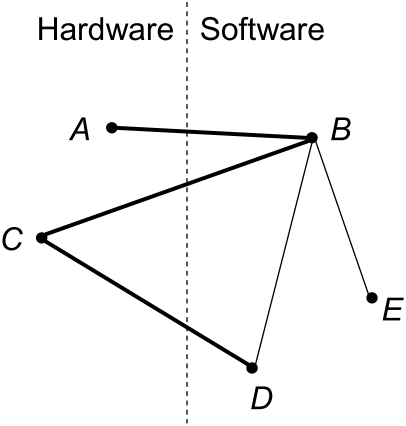
\includegraphics[width=0.4\textwidth]{img/partitioning.png}
         \caption{Representação Geral de um Particionamento em um grafo não direcionado.
         Os $\bullet$ (pontos) representam componentes da aplicação e as --- (linhas) seus respectivos fluxos de comunicação.
         A linha tracejada representa a divisão de níveis entre eles, sendo este \hs.
         Fonte: \citet{Mann2007}.}
         \label{fig:f4-4}
         \end{figure}
\end{comment}
         %\section{Declaração Formal do Problema}
         %	Descreveremos problema segundo a definição de \citeauthor{Arato2005, Mann2007} a seguir.

         %\section{Solução analítica para particionamento}
         %\section{Visão Analítica Para o Particionamento}


      \subsection{Declaração do Problema} \label{sec:declaracao_problema}
         Nesta seção serão apresentadas as declarações matemáticas do problema de agrupamento de instruções em recursos e seus mapeamentos em \hardware\ ou \software, ou seja, o particionamento \hs.
         %Segundo \cite{Sass2010}, a forma mais comum de transcrever é descrever manualmente o \core\ com um HDL utilizando \design\ referencial de \software\ como especificação, método utilizado para descrever o problema.

         No particionamento, muitos problemas práticos impactam diretamente na performance do sistema.
         Nem todos os problemas podem ser incorporados num modelo analítico \cite{Wang2016}, e por isso, só podemos esperar que as soluções matemáticas produzam uma uma resposta aproximada ao problema de particionamento ao utilizar a declaração formal.

         Muitas das entradas do modelo são estimadas ou aproximações no qual futuramente degrada a fidelidade de resultados.
         %%Este é um fato relevante pois com isso, resolvendo o problema de particionamento `no papel', tem-se um particionamento que é próximo ao ótimo.
         %%Assim, cabe ao \designer\ ser habilidoso em usar os guias e projetar uma solução mais refinada.
         Dessa forma, é mais eficiente usar uma combinação de técnicas \textit{ad hoc} e matemáticas para encontrar uma solução ótima ou aproximada do que simplesmente confiar numa intuição.


         %\begin{comment}
         %\section{Declaração do Problema}
         Já descrito as ferramentas matemáticas necessárias para descrever o problema fundamental do particionamento no Capítulo \ref{chap:revisao_bibliografica}, pode-se então descrever formalmente o problema em termos de variáveis. % e descrever um algoritmo \todo{algorit?}para encontrar uma solução aproximada.
         %
         A ideia básica consiste em encontrar um particionamento para todos os blocos básicos de uma aplicação e então separá-los em \hs.
         Formalmente, procura-se por uma partição $ \mathcal{P} $ de todos os blocos básicos $ U $ de uma aplicação (Equação \ref{eq:bigcup}).
         %
         %$$ U = \bigcup_{C \in \mathcal{C}} B(C) $$
         %
         %$ C = (B,F) $
         Definida a partição e o universo, tem-se então um subconjunto $ \mathbb{C}\ |\ \mathbb{C} \subseteq U $, onde $ C \in \mathcal{C} $ é um vértice de um grafo de \design\ referencial de \software\ $ \mathcal{A} = (\mathcal{C}, \mathcal{L}) $ (oriundo da Equação \ref{eq:a}).
         O conjunto $ \mathbb{C} $, chamado conjunto de candidatos, contém todos os recursos arquiteturais potenciais, ou seja, o subconjunto de $ U $ que é esperado para melhorar a performance do sistema se implementado em um \hardware\ reconfigurável.
         Devido ao limite de recursos, deve-se refinar para o subconjunto $ \mathbb{D} \subseteq \mathbb{C} $ que maximiza nosso métrica de performance.
         Assim
         \begin{equation}
            \begin{array}{rrcl}
            \text{max}                 & \Gamma ( \mathbb{D})               & ~   & ~                \\
            subject\ to & \sum_{i \in \mathbb{D}} \vec{r}(i) & < & \vec{r}_{FPGA}
            \end{array}
            \label{eq:constraints}
         \end{equation}
         %
         Descrevendo algoritmicamente, uma abordagem seria encontrar todas as partições de $ U $, sintetizando e \textit{profiling} cada partição, e então, quantitativamente avaliar cada $ \Gamma $.
         Entretanto, este é um problema linear inteiro devido à natureza de alocação e utilização dos recurso físicos do FPGA. %(Seção \ref{sec:pli})

         A seguir, será descrito como é feito uma abordagem para tal, seguindo estudos de \citet{Arato2003, Wang2016}.

\begin{comment}

      \subsection{Abordagem Heurística}
         O problema de particionamento é essencialmente uma questão indireta de manipulação de parâmetros $ p(i) $ e $ \gamma(i) $ (tempo gasto em e ganho de performance, respectivamente) pelo rearranjo do particionamento $ \mathcal{X} $.
         Então seleciona-se os elementos de $ \mathcal{X} $ que satisfaz as restrições de recurso e maximiza a performance do sistema $ \Gamma $, Equação \ref{eq:constraints}.

         Uma metodologia heurística que pode ser aplicada seria iniciar a partição natural provida pelo \design\ referencial de \software, ou seja, utiliza-se as sub-rotinas de uma aplicação original.
         %
         Utilizando a ferramenta de \textit{profiling}, lista-se as sub-rotinas em ordem decrescente em tempo e verifica-se as que possuem maior valor $ p $.
         O valor de $ \gamma $ será estimado pela performance esperada a partir da implementação em \hardware\ e ao final, tem-se um ganho estimado do sistema para cada sub-rotina.

         Em seguida, quer-se manipular iterativamente a partição $ \mathcal{X} = \{ X_0, X_1, X_2, ...\} $ criando um novo subconjunto de blocos básicos por meio de operações de casamento e movimentações de blocos.
         A ideia em realizar alterações iterativas é encontrar mudanças que podem alterar os valores da fração $ p $ ou o valor de $ \gamma $.

         Num \wearable\ que tenha como procedimentos cálculos matemáticos, verificar quais funções possui maior impacto na sua execução e assim, realizar uma busca a fim de encontrar uma partição de procedimentos que poderiam ser implementados em um acelerador aumentando possivelmente o \speedup\ do sistema.

         Para aumentar o ganho performance de recurso $ \gamma (i) $ utilizando abordagens heurísticas, necessita-se verificar o grafo de controle de fluxo do recurso e avaliar se uma mudança o tornará mais sequencial ou paralelo.

         Uma forma de reduzir a fração de tempo gasta de uma sub-rotina é torná-la maior na quantidade de recurso alocada a ela.
         Por exemplo, casando vários blocos básicos num único bloco.
         Isso pode ser alcançado procurando por relações no grafo de chamadas ou, após a manipulação, por relacionamentos no grafo de controle de fluxo que conecta subconjuntos.

         %Frequentemente, algoritmos que são inerentemente sequenciais, ou seja, uma forte dependência em seu fluxo ou dependências de controle, possuem melhor performance em processadores, por este não ter a sobrecarga de configurações de transistores e de possuírem melhor gerenciamento de energia nessas circunstâncias.
         %Ou seja, simplesmente adicionar blocos básicos a qualquer custo pode ter um efeito indesejável de aumentar o comportamento sequencial do recurso, reduzindo o valor de $ \gamma $.
         %Entretanto, se um componente utilizar-se de menos recursos, então possui potencial de aumentar seu ganho de desempenho pela simplicidade.

         Exemplificando de uma forma mais abstrata, considera-se uma sub-rotina $ X $ e quebrando-a em duas sob-rotinas $ X – X' $ e $ X' $, onde a sub-rotina $ X – X' $ invoca $ X' $.
         Então se $ X' $ extrai partes de $ X $ que podem ser melhoradas em nível de \hardware\ deixando a parte sequencial em $ X – X' $, então $ \gamma $ de $ X' $ será maior que $ \gamma $ de $ X $ original e provavelmente necessitará de menos recursos.

         %A lei de Ahmdal tenta sempre aumentar a fração de tempo gasto na porção de código que acaba de ser melhorada.
         %No entanto, quando limitado os recursos, nem sempre é melhor.

         Com isso, é importante notar que qualquer mudança no subconjunto pode afetar a performance para melhor ou pior.
         Em geral, heurísticas trabalham examinando os grafos da aplicação e então fazendo alterações incrementais ao subconjunto de uma partição.
         Tais mudanças são guiadas pela tentativa de diminuir o tempo gasto em uma sub-rotina não aumentando dramaticamente seus recursos ou decrescendo sua performance; e a tentativa de melhorar a performance sem aumentar o tempo gasto em uma sub-rotina.

\end{comment}


   %\section{Metodologia Proposta}
   \section{Proposta de Procedimento Analítico} \label{sec:proposta}

      Como conclusão deste capítulo, será formulada uma proposta de metodologia analítica baseada nos conceitos propostos pela literatura, com o foco em componentes procedurais integrados à sistemas \wearables.
      %E com isso, o trabalho consiste em desenvolver seus respectivos grafos e realizar o particionamento a fim de encontrar uma solução aproximada, respeitando os seus requisitos de funcionamento.
      %
      Tal metodologia, apresentada pelo Algoritmo~\ref{alg:proposta}, será considerada apenas como uma orientação para os passos a serem realizados, sendo então, uma proposta representativa do processo a ser realizado para a análise e decisão de particionamento.

      \begin{algorithm}[h]
         \SetKwData{itt}{it}
         \SetKwData{pl}{partition\_list}
         \SetKwData{complexSet}{how\_complex\_set\_is}
         \SetKwData{md}{matriz\_dados}
         \SetKwData{complexSet}{how\_complex\_set\_is}
         \SetKwFunction{graph}{makes\_graph}
         \SetKwFunction{porte}{analyses\_complex\_set}
         \SetKwFunction{synth}{synthesizes}
         \SetKwFunction{resources}{resources\_used}
         \SetKwFunction{die}{die\_used}
         \SetKwFunction{energy}{energy\_spent}
         \SetKwFunction{profiling}{profile}
         \SetKwFunction{performance}{performance\_analysis}
         \SetKwFunction{factor}{complexity\_factor}
         \SetKwFunction{ilp}{integer\_linear\_solve}
         \SetKwFunction{heuristic}{heuristic}
         \KwIn{a project description.}
         \KwOut{a partition solved.}

         %\BlankLine
         \Begin{

            \BlankLine
            \profiling{}\;
            \BlankLine

            \tcp{extration project analyses}
            \graph{Flow Control Graph}\;
            \graph{Call Graph}\;
            %\complexSet $\leftarrow$ \porte{}\tcp*{verify if it is a big project}

            \BlankLine

            \If{exist partitions that can be synthesized}{
               \ForEach{partition project:\itt $\in$ \pl}{
                  \synth{\itt}\;
                  \BlankLine
                  \resources{\itt}\tcp*{analysis after synth}
                  \die{\itt}\;
                  \energy{\itt}\;
                  %\BlankLine


                  \performance{\itt}\;
               }
               \BlankLine

               %\uIf(\tcp*[f]{verify if it is a small project}){\factor{\complexSet}}{
                  \ilp{\pl}\tcp*{analyse quantitatively each $ \Gamma $}
               %}
               %\lElse{
                  %\heuristic{\pl}\;
               %}
            }
         }
         \caption{Metodologia para avaliação de \wearables.}
         \label{alg:proposta}
      \end{algorithm}

      Apresentado o procedimento metodológico, a seguir será listada cada função pertencente à metodologia acima, descrevendo suas funções e seu propósito no trabalho para a obtenção dos objetivos.
      Para um melhor compreendimento, serão divididos em quatro seções, sendo elas: visualização do projeto, síntese, análise de síntese, particionamento.

      \begin{comment}
      Dessa forma, o primeiro passo proposto é a análise do sistema por meio de testes em nível de \software, ou seja, o sistema realizado sobre um processador.
      Como exibido no Algoritmo~\ref{alg:manual}, os processos se baseiam na construção e análise do sistema em um processador.
      Deve-se realizar a construção de seus gráficos para seu entendimento (linhas 2 e 3), e em seguida (linha 4) uma avaliação do porte do sistema, item essencial para a escolha do algoritmo propício ao realizar o particionamento, caso exista.
      Nas linhas 5, 6 e 7 são análises feitas a partir da execução do mesmo numa plataforma, obtendo seu \profile, performance e gasto energético respectivamente.

      \begin{algorithm}[h]
        %\KwResult{Write ere the result }
        \SetKwData{md}{matriz\_dados}
        \SetKwData{complexSet}{how\_complex\_set\_is}
        \SetKwFunction{graph}{makes\_graph}
        \SetKwFunction{porte}{analyses\_complex\_set}
        \SetKwFunction{energy}{energy\_spent\_analyses}
        \SetKwFunction{performance}{performance\_analyses}
        \SetKwFunction{profiling}{profile}
        \KwIn{software reference design.}
        \KwOut{software analyses.}
        \BlankLine
        \tcc{this algorithm happens in a soft core system without anyone accelearator}
        \BlankLine
        \Begin{

           \tcp{extration project analyses}
           \graph{Flow Control Graph}\;
           \graph{Call Graph}\;
           \complexSet $\leftarrow$ \porte{}\tcp*{verify if it is a big project}

           \BlankLine

           \tcp{physical project analyses}
           \profiling{}\;
           \performance{}\;
           \energy{}\;
        }
        \caption{Processos manuais para análise inicial do dispositivo.}
        \label{alg:manual}
      \end{algorithm}
\end{comment}


      \begin{enumerate}
         \item Procedimentos para visualização geral do projeto.
         Por meio dos dados do \profile\ e a construção dos grafos, é possível ter uma visão geral, verificando se o sistema possui possíveis seções de processamentos críticos para a realização de particionamento \hs.
         As funções presentes são:

         \begin{itemize}
            \item \texttt{profile():}
               procedimento referente à Seção~\ref{sec:profile}.
               Realiza-se uma análise de tempo gasto em cada procedimento do projeto, apresentando-a ao final de sua execução.
               Com os resultados, é possível ver locais onde existe um tempo maior de processamento gasto ou de recursos utilizados indicando uma verificação detalhada sobre este a fim de candidatá-lo para uma implementação em \hardware;

            \item \texttt{makes\_graph(}\textit{type}\texttt{):}
               constrói-se grafos relativos ao projeto, sendo estes de acordo com o tipo especificado no parâmetro.
               A construção do grafo segue como descrito na Seção~\ref{sec:GCF} na qual procura-se por seções de códigos compondo-os em blocos, compreendendo o fluxo do algoritmo e consecutivamente os procedimentos de chamadas.
               O parâmetro simboliza a especificação de qual tipo de grafo será construído, sendo ele um grafo de controle de fluxo (Seção~\ref{sec:GCF}) ou grafo de chamada (Seção~\ref{sec:gc}), que como já explicado, necessita do anterior para sua construção;
         \end{itemize}

         \item \texttt{synthesizes():}
            caso exista uma possibilidade de particionamento, análise obtida pelo \profile, visualização do grafo e obtenção de uma lista de candidatos, realiza-se então o procedimento de geração de HDL para o desenvolvimento de aceleradores em \textit{hardware} reconfigurável e sua análise de performance e gastos tanto de energia quanto de recursos;

         \item Após a execução do processo de síntese realizado junto com a ferramenta sintetizadora assistida pelo computador, é possível obter vários dados analíticos de alocação de recursos como quantidade de elementos lógicos utilizados, pinos virtuais e físicos, quantidade de bits de memória, além de vários outros.
         E com a sua sintetização na plataforma, também é possível obter a avaliação de consumo energético, \profile\ e performance.
         Estes são representados pelos métodos abaixo na qual, aplica-se a cada componente sintetizado separadamente.
         \begin{itemize}

            \item \texttt{resources\_used():}
               quais e a quantidade de recursos alocados para utilização no projeto de geração de aceleradores.
               A alocação de muitos recursos implica num gasto maior de energia criando um \textit{trade-off} a ser analisado;

            \item \texttt{die\_used():}
               tamanho do \textit{die} utilizado para o projeto do acelerador.
               Sistemas \wearable\ possuem como requisito a sua miniaturização, impedindo que seu uso limite a capacidade de locomoção, usabilidade ou conforto do usuário, por exemplo;

            \item \texttt{energy\_spent():}
               valores energéticos do uso do recurso implementado, incluindo os módulos pertencentes a ele como memórias, DSPs e quaisquer outros que estejam integrados à plataforma;

            \item \texttt{performance\_analysis():}
               comparação das implementações em \hardware\ sobre os recursos em nível de \textit{software}, ou seja análise de performance.
         \end{itemize}

         \item \texttt{integer\_linear\_solver():}
            após realizado todas as análises individuais acima, inicia-se o processo de procura de uma solução de particionamento que obtenha bons resultados nos requisitos de um sistema \wearable.
            Dessa forma, é realizado uma avaliação por meio de um \textit{solver} linear inteiro segundo os dados obtidos.
            Com o \textit{solver}, é possível realizar uma busca a procura de um particionamento que atenda a quantidade máxima de restrições exigidas por um \wearable.
      \end{enumerate}


      %Conclusão
      Assim, o trabalho consiste numa metodologia na qual aborda o particionamento para dispositivos \wearables, partindo de uma análise de execução do \software, candidatando alguns procedimentos para sua sintetização e assim a avaliação destes segundo os recursos utilizados para a completude de suas tarefas o que chamamos de particionamento, consistindo da procura de um conjunto que traga melhor desempenho no seu uso. Tudo isso, utilizando recursos disponibilizados pela plataforma em \hardware.
      %O Algoritmo~\ref{alg:proposta} tem como o objetivo a demonstração do passos necessários para o compreendimento do sistema a ser analisado e consecutivamente a sua partição em busca do aprimoramento da sua performance.

    %!TEX root = ../main_text.tex

\chapter{Metodologia Proposta} \label{chap:met2}
   %bla bla bla
   Apresentado o problema de particionamento, sua importância, será apresentado uma abordagem para o projeto de sistemas computacionais \wearables\ e aplicações deste em sistemas hipotéticos.

   % Tem vários trabalhos, mas sem wearable
   Como foi possível perceber no Capítulo Trabalhos Relacionados (Capítulo \ref{chap:relacionados}), existem vários trabalhos em sistemas computacionais embarcados, entretanto, nenhum que abordasse o tema para \wearables.
   %justificativa de bateria e die
   Partindo deste pressuposto, esta pesquisa propõe o estudo de dispositivos \wearables\ e a aplicação de técnicas de particionamento a fim de obter um desempenho melhor para estes.

   % pesquisa com fourier
   %Sendo assim, será realizado uma pesquisa de particionamento sobre algoritmos comumente utilizados em sistemas \wearables\ de forma a verificar seus gastos energéticos e recursos utilizados em \hardware, como por exemplo o cálculo da Transformada de Fourier, fórmula utilizado em situações cabíveis em dispositivos \wearable\ como análise, filtros, reconstrução e compressão de imagens, por exemplo.

   %metodologia
   A metodologia proposta baseia-se em procedimentos que utilizam as técnicas descritas neste documento.
   No Capítulo \ref{chap:design} foi descrito os principais métodos utilizados neste trabalho, e ao final foi apresentado um procedimento na qual a metodologia usará como base.
   O método consiste unicamente na organização dos conceitos discutidos a fim de obter uma análise sistemática do projeto e assim, realizar o particionamento a procura de melhorias.
   A diferença entre a análise metodológica de um exemplo hipotético e de um dispositivo real é que com o real, todas as principais funções do dispositivo são consideras e assim, a quantidade de procedimentos a serem considerados para o particionamento \hs\ seria maior, criando um leque maior de possibilidade para análise.
   Assim, para demonstração da metodologia, será realizada sua aplicação para a análise de dois dispositivos \wearables\ hipotéticos descritos nas Seções~\ref{sec:hip1} e \ref{sec:hip2} a seguir.


   \section{\Wearable\ Hipotético 1: Mão Biônica} \label{sec:hip1}

      \paragraph{Apresentação}
         % Exemplificação teórica
         %A seguir será apresentado uma situação hipotética na qual a metodologia do tema pesquisado seria aplicada.
         % porque do problema
         Como já é de conhecimento, o ser humano, bem como todos os outros animais, usa de seus músculos corporais para as tarefas cotidianas como andar, comer, etc.
         Com o estímulo ordenado dos músculos, é possível realizar atuações até mais complexas como segurar um objeto pelas mãos ou mesmo, ter controle sobre um automóvel ou realizar uma performance artística/musical.
         %Todos estes necessitam de uma ordenação e coordenação dos movimentos realizados.
         %apresentação do wearable
         Assim, uma situação de uso de \wearable\ é, ao invés do usuário utilizar de suas próprias mãos para realizar alguma atividade como a de segurar um objeto, com a adição de um sistema \wearable, seria possível intermediar a atuação final (tomar algo pelas mão), com a leitura da tensão elétrica muscular do usuário ao longo do tempo, a fim de substituir a atuação de sua mão por meio de atuadores mecânicos artificiais, como mostra a Figura~\ref{fig:maobionica}.

         \begin{figure}[h] \centering
            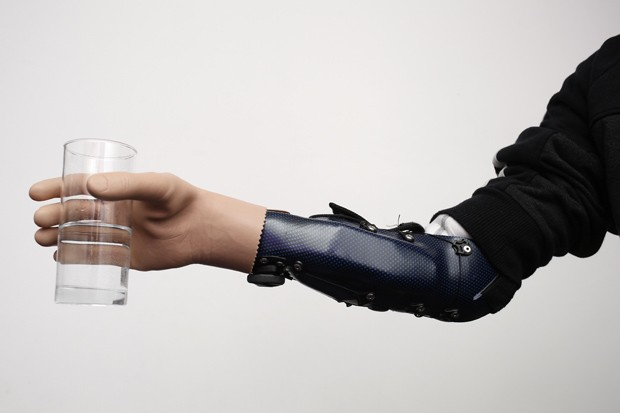
\includegraphics[width=0.7\textwidth]{img/maobionica.jpg}
            \caption{Demonstração de uma mão biônica. Fonte: \url{https://goo.gl/96PURB} Acesso: 30/07/2017.}
            \label{fig:maobionica}
         \end{figure}

         %técnico
         Descrevendo-o de uma forma mais técnica, o \wearable\ deve ser capaz de realizar leituras eletromiográficas%
         \footnote{Técnica na qual realiza o monitoramento de atividades elétricas das células musculares.},
         interpretá-las de acordo com um pretexto e realizar a atuação.
         Um pseudo-algoritmo é apresentado em Algoritmo~\ref{alg:wearable1}.
         %
         % particionamento no wearable apresentado
         Pode-se supor que o dispositivo foi inteiramente construído em uma solução em \software\ com a justificativa de projeto de uma construção mais simples.
         Assim sendo, o particionamento \hs\ entra com o papel de analisar o projeto a fim de buscar por combinações de particionamento que apresentem melhorias em performance ou no gasto energético ao estado atual.
         A análise é importante mesmo para projetos que já possuam aceleradores em \hardware\ em seu projeto pois a verificação atua como uma forma de validação e confirmação de sua performance como uma solução aproximada do ótimo.

         \begin{algorithm}[h]
            \SetKwData{md}{matrix\_data}
            \SetKwData{mdp}{matrix\_data\_preprocessed}
            \SetKwData{eb}{buffer\_state}
            \SetKwData{ea}{state\_before}
            \SetKwData{sx}{sensor$_i$}
            \SetKwFunction{leSensores}{reads\_sensors}
            \SetKwFunction{preprocess}{pre\_process}
            \SetKwFunction{process}{processes}
            \SetKwFunction{atuacao}{operates}
            \SetKwFunction{bu}{backup}

            \KwIn{sensors reads.}
            \KwOut{acting.}
            \BlankLine

            \Begin{
               \BlankLine
               \tcp{statements}
               \sx\tcp*{$i$ information's source}
               \md\tcp*{data's matrix before handling}
               \mdp\tcp*{data's matrix after handling}
               \eb\tcp*{last state applied and current}
               \ea\tcp*{generated state to be compared}
               \BlankLine

               \While{wearable mode on}{
                  \md $\leftarrow$ \leSensores{\sx}\;
                  \mdp $\leftarrow$ \preprocess{\md}\;

                  \BlankLine

                  \tcp{process the datas}
                  \If{\eb $\leftarrow$ \process{\mdp} $\ne$ \ea}{
                     \tcp{operates}
                     \ea $\leftarrow$ \eb\;
                     \atuacao{\ea}\;

                     \BlankLine
                     \bu{}\tcp*{saves the data persistently}
                  }
                  \BlankLine
               }
            }

            \caption{\Wearable\ 1 - Procedimentos realizados pelo dispositivo \wearable\ denominado Mão Biônica.}
            \label{alg:wearable1}
         \end{algorithm}

         Suponha então que deseja-se realizar uma avaliação de particionamento \hs\ de um dispositivo \wearable\ que atua por meio de tais sinais eletromiográficos.
         %O primeiro passo a ser realizado é a construção do grafo de chamada do projeto, exibido no próximo tópico.

      \paragraph{Análise Usando \Profile}
         O primeiro procedimento a ser realizado para a obtenção de informações de projeto e execução do programa é com a execução de um \software\ que faça o seu \profile.
         Ao realizar esta tarefa, obtêm-se resultados de tempo de execução dos principais procedimentos do projeto, listados de forma ordenada por tempo gasto, como já descrito na Seção \ref{sec:profile}.
         
         Feito esta análise, é construído o grafo de chamada de acordo com a especificação de funcionamento do projeto.

      \paragraph{Grafo}
         A partir do pseudo-algoritmo dado e da análise \profile, é possível gerar o grafo de chamada, exibido pela Figura~\ref{fig:graph_w1}.
         %explicação grafo
         Como descrito na Seção \ref{sec:GCF}, é realizado uma análise no projeto verificando os códigos e funções, gerando o seu respectivo grafo de chamada.
         %Como este é um exemplo hipotético, gerou-se um grafo mais simples, mas que ainda representa o real funcionamento do dispositivo.

         \begin{figure}[h] \centering
            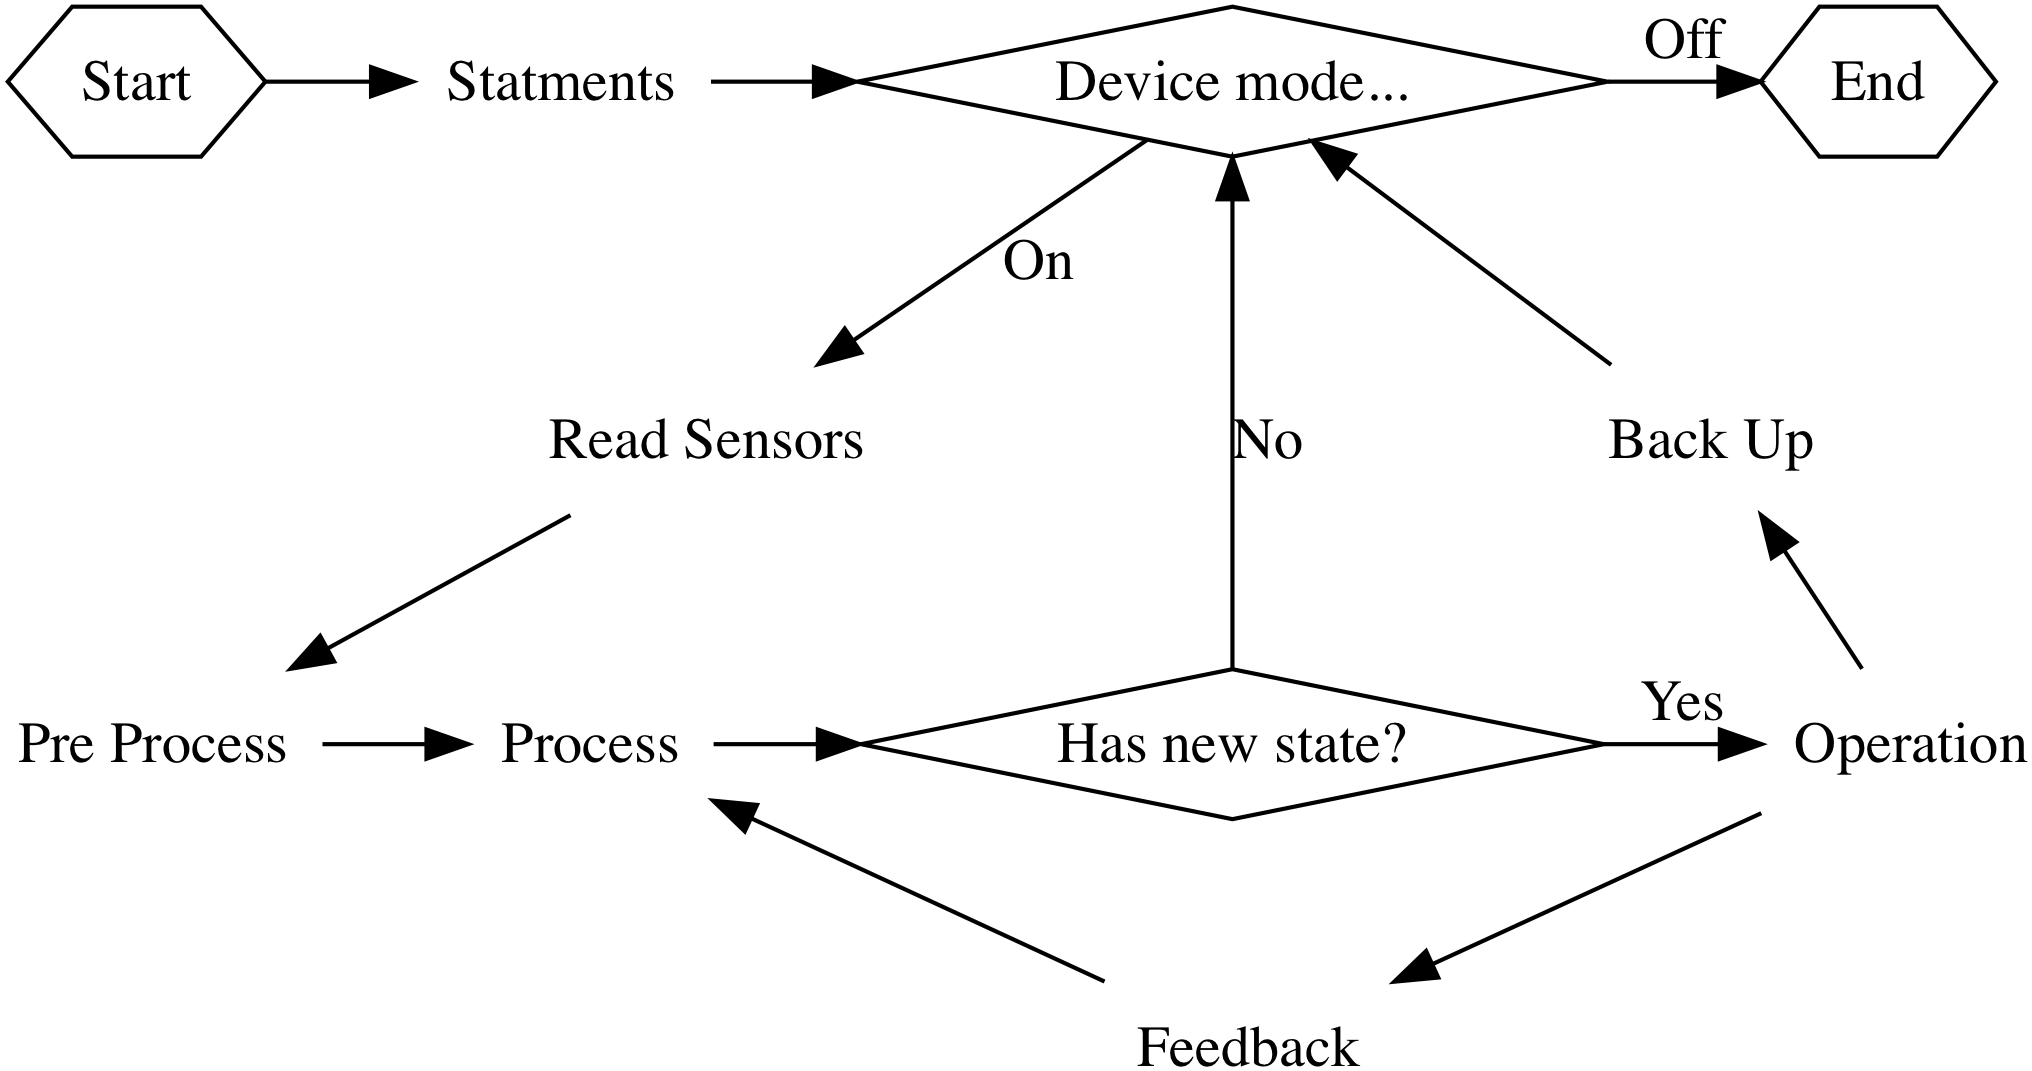
\includegraphics[width=0.9\textwidth]{img/graph_wearable.png}
            \caption{Exemplificação de um grafo de chamada para o exemplo.}
            \label{fig:graph_w1}
         \end{figure}

         %explicando o grafo
         %start
         O processo representado pelo grafo da Figura~\ref{fig:graph_w1} inicia-se pelo estado de formato hexágono com etiqueta \textit{start}.
         %statment
         Ao iniciar o dispositivo, é realizado as inicializações de ambiente, definidas pelo estado seguinte \textit{statments}, realizando todas as definições prévias para seu uso.
         Este processo é unicamente para inicialização do equipamento, redefinindo todos os estados da última operação ou de um estado específico de inicialização.
         %if 1
         Em seguida, tem-se o primeiro losango indicando uma verificação de estado.
         Neste, verifica-se se o dispositivo entrou-se em modo de desligamento, se sim, desligando-o de forma segura.
         %process
         Caso contrário, realiza leituras eletromiográficas, o pré-processamento delas e em seguida o processamento dos dados.
         %if 2
         Após processado, é verificado se existe um novo estado de acordo com os valores lidos.
         %operacao
         Se este novo estado é distinto do anterior, então o dispositivo deve realizar a operação de alteração da atuação para este novo, além do armazenamento deste em forma persistente para inicialização, caso estabelecido e o processo é reiniciado na verificação de de dispositivo ligado.
         Neste também é realizado a leitura de \textit{feedback} da atuação retornando-o para o processamento para avaliar o erro e gerar uma resposta para tal.

         % grafo hipotético vs real
         O grafo gerado deste exemplo apresentado é uma solução simplista pelo fato de ser inteiramente hipotético.
         Com um exemplo real, seria possível ter um detalhamento maior no grafo, já que este teria informações suficientes sobre os procedimentos do dispositivo para compreendimento.

         Ao concluir a construção do grafo do sistema \wearable\ e analisá-lo, consegue-se ter conhecimento de grupos procedurais importantes e assim, consequentemente separá-las em módulos.
         %Como \wearables\ baseiam-se em avaliação, interpretação e ação, será aplicada uma identificação de grupo para facilitar o entendimento de cada módulo do dispositivo.
         Foram denominados três grupo para a organização dos procedimentos, sendo eles Leitura, Processamento e Atuação, e serão descritos a seguir.

         \begin{description}
            \item [Módulo de Leitura:]
            A leitura é realizada por meio de um sensor muscular na qual obtém sinais eletromiográficos, ou seja, um sensor de eletromiograma.

            Não só como a leitura mas a interpretação dos sinais elétrico depende diretamente da natureza dos dados sensoriais obtidos pelo eletromiograma, um pré-processamento de tais dados é um fator está relacionado diretamente com a obtenção de informação do conjunto de dados.
            Então, supondo que o dispositivo \wearable\ também necessite de um pré-processamento dos dados para filtragem e preparação para o processamento central de fato, este estaria incluso dentro do módulo de leitura, enviando-os em seguida para o processamento central.
            
            O grupo será composto pelos procedimentos: \texttt{Statments}, \texttt{Read Sensors} e \texttt{Pre Process}.

            \item [Módulo de Processamento Central:]
            Com os dados já trabalhados para serem utilizados de forma mais clara, o próximo passo a ser realizado é a interpretação destes de acordo com um pretexto pré-estabelecido pelo projetista e assim tomar uma decisão sobre este.
            Dessa forma, é realizado uma verificação de padrões do conjunto de dados recebido e a alteração de estado de atuação caso necessário.

            Caso exista tal mudança, especificar qual e passar isso para o próximo módulo, a atuação.
            Caso contrário realiza novas leituras de dados, já que não obteve nenhuma alteração de estado de atuação.

            Para o projeto ser mais responsivo, seria ideal obter também um \textit{feedback} relativo à atuação, criando uma correlação mais precisa entre os dados lidos de sensores musculares com o estado do atuador e sua atuação.
            O \textit{feedback} seria relacionado à completude da atuação, verificando se a atuação foi realmente executada como esperado e, caso negativo, encontrar o valor de erro para a sua tentativa de correção, processamento a ser realizado neste módulo.
            
            Composto pelos procedimentos: \texttt{Process} e \texttt{feedback}.

            \item [Módulo de Atuação:]
            Meio no qual realiza-se a atuação, segundo implicação oriunda do processamento central.

            Neste, também seria realizado as leituras de \textit{feedback}, enviando-os para o módulo de processamento central.
            
            Composto pelas funções: \texttt{Operation} e \texttt{Back Up}.
         \end{description}

      Após feito o \profile\ e o desenvolvimento do grafo, deve-se verificar quais procedimentos são candidatos a serem sintetizados para análise de performance.
      Procedimentos que realizam cálculos matemáticos repetitivos, ou que são executados ocasionalmente são excelentes candidatos já que pode-se utilizar os recursos de \hardware\ para o processamento com maior vazão de dados ou o acionamento e desligamento do recursos quando não utilizado, respectivamente às situações apresentadas.

      \paragraph{Análises de Síntese}
         Construído o grafo e verificado os candidatos ao particionamento por meio do \profile, realiza-se então a sintetização de todos os procedimentos candidatos bem como suas análises de uso de recursos e performance.
         
         Todos os procedimentos do projeto apresentado são candidatos a serem sintetizados e analisados.
         São procedimentos que também necessitam de resposta imediata ao estímulo dado, aproximando ao máximo à uma atuação instantânea realizada pelos membros musculares naturais.
         Isso pois, todos os procedimentos podem ser executados sem a presença de um microcontrolador, usando recursos de uma máquina de estados para controle por exemplo.
         
         Dessa forma, como são candidatos, serão sintetizados, analisados e comparados com os procedimentos realizados via \software\ por meio de um microcontrolador.
         
      \paragraph{\textit{Solver}}
         Obtida as análises de cada componente em nível de \software\ e \hardware, utiliza-se de \textit{solvers} para encontrar uma solução boa.
         
         No Capítulo \ref{chap:relacionados}, existem inúmeras aplicações que utilizam desde métodos exatos baseado em programação inteira linear até metaheurísticas.
         Dessa forma, após a aplicação do método \textit{solver}, obteremos um particionamento solucionado pelo solver de acordo com as restrições de recursos impostas.


   \section{\Wearable\ Hipotético 2: Capacete para Segurança de Ciclistas} \label{sec:hip2}
      \paragraph{Apresentação}
         Outro exemplo de \wearable\ e suas análises está em propor um capacete desenvolvido para a segurança de ciclistas.
         O hipotético propósito deste seria fornecer um auxílio para a segurança do usuário, junto com dados estatísticos de corrida com a bicicleta.
         
         O equipamento seria utilizado para verificar situações na qual um veículo estaria se aproximando do usuário pela suas costas de forma a gerar uma colisão, local sem visibilidade constante pelo ciclista.
         Dessa forma, o capacete poderia avisar o ciclista para manter cuidado e tomar uma atitude segura enviando alguma informação para seu \textit{smartphone} ou para algum dispositivo \textit{wearable} acoplado ao seu corpo como uma pulseira.
         Ambos dispositivos poderiam passar a informação para o ciclista por meio de estímulos visuais ou físicos como luzes ou vibrações ou, pensando num equipamento mais tecnológico, um aviso em um óculos com realidade aumentada, por exemplo.
         
         Como já dito, além da prevenção de acidentes, o equipamento poderia ainda suportar procedimentos que realizem a obtenção e envio de dados de atividades físicas do usuário como distância percorrida, tempo de atividade e na qual, após o processamento dos dados, a geração de informações como velocidade média, estimação de calorias queimadas, entre outras.
         Isso, enviando para um aplicativo no seu telefone móvel por meio de uma conexão sem fio.

         O projeto, em termos técnicos, seria composto de sensores capazes de realizar a verificação de objetos volumosos e sua distância em relação ao ponto atual do ciclista.
         Ao avistar um objeto aproximando, por meio de uma conexão sem fio, o capacete enviaria um pacote de notificação para os dispositivos acoplados ao corpo do usuário avisando-o que está em uma situação de perigo.
         Além de tais dispositivos, o capacete poderia reagir também com sinais luminosos situados nele próprio, a fim de alertar o ciclista e/ou também o motorista mostrando que existe um algo em sua frente que na qual, necessita de sua atenção para não haver uma colisão.
         
         Já os dados de atividade física podem ser obtidos por meio de acelerômetros, giroscópios, GPS, RTC, na qual permitem a interpretação dos dados por meio de cálculos, gerando informações de posicionamento, orientação, velocidade, tempo, além de gasto energético, velocidade média percorrida e até um sistemas de conquista de metas.
         É possível desenvolver um sistema na qual relacione todos os sensores como o exemplo de que o sensor de risco só seja ativado quando o ciclista esteja se movimentado, situação na qual utiliza os sensores de distância e acelerômetro.
         Os dados de todos os sensores seriam gravados em uma memória não volátil para acesso e sincronização com um \textit{smartphone} futuramente.
   
         A seguir será exibido vários procedimentos responsáveis por demonstrar a execução do dispositivo.         
         O primeiro, Algoritmo~\ref{alg:wearable2_leituras}, exibe o procedimento para leitura de sensores e o armazenamento de tais informações em memória não-volátil.
         Caso verificado que existe uma situação de risco acontecendo por meio da leitura, também será realizado o envio de um sinal de interrupção para o controlador a fim de que os procedimentos de aviso sejam realizados.
   
         \begin{algorithm}[h]
            \SetKwData{data}{datas}
            \SetKwData{typew}{type\_warning}
            \SetKwData{sx}{sensor$_i$}
            \SetKwFunction{leSensores}{reads\_sensors}
            \SetKwFunction{preprocess}{pre\_process}
            \SetKwFunction{process}{processes}
            \SetKwFunction{atuacao}{operates}
            \SetKwFunction{finterrupt}{does\_interruption}
            \SetKwFunction{bu}{backup}
            
            \BlankLine
            \KwIn{sensors reads.}
            \KwOut{backups and interruptions signals.}
            \BlankLine
   
            \Begin{
               \tcp{statements}
               \sx\tcp*{$i$ information's source}
               \data\tcp*{data's matrix before handling}
               \typew\tcp*{type of warning to do to user}
               \BlankLine
   
               \While{wearable mode on}{
                  \data $\leftarrow$ \leSensores{\sx}\;
                  \BlankLine
   
                  \tcp{process the datas}
                  \typew $\leftarrow$ \process{\data}\;
                  
                  \BlankLine
                  \If{\typew $=$ dangerous}{
                     \finterrupt{\typew}\;
                  }                  
                  
                  \BlankLine
                  \bu{\data}\;
   
                  \BlankLine
               }
               \BlankLine
            }
   
            \caption{\Wearable\ 2 - Procedimento que realiza leituras de sensores e armazena seus dados em memória não-volátil.}
            \label{alg:wearable2_leituras}
         \end{algorithm}
         
         Dessa forma, o Algoritmo~\ref{alg:wearable2_leituras}, na linha 6, realiza leitura dos sensores e em seguida verifica se existe alguma gravidade na situação.
         Se positivo, gera o sinal de interrupção.
         Como esse módulo é um módulo independente e gerador de interrupções, ao realizar uma, não necessita de criar-se um bloqueio em seus procedimentos. 
         Isso significa que o módulo poderá continuar com suas instruções de ler, analisar e gravar os dados, independente do controlador estiver ou não com interrupção.
         
         Após o controlador receber a interrupção, inicia-se o processo do Algoritmo~\ref{alg:wearable2_interrupcao} para tratá-la.
         A função \texttt{does\_interruption} é estimulada sempre que um sinal de interrupção é ativado ou mantido ativo.
         %buffer
         Após iniciada, tipo da interrupção é gravado numa variável auxiliar com nome \texttt{buffer\_type\_warning}.
         Isso é importante pois, caso a interrupção seja retirada no meio da função, não permita a possibilidade de um dispositivo realizar o alerta e outro não, criando uma confusão no compreendimento do usuário sobre sua situação.
         Como já dito, o processo de alerta ficará ativo enquanto a interrupção estiver ativada e assim, como exibido na linha 4, o procedimento continuará em repetição enquanto o valor não ser alterado, na linha 10.
         %conexao
         O primeiro passo a se fazer ao receber a interrupção é verificar se o capacete possui conexão sem-fio com os equipamentos que possuem suporte (como o \textit{smartphone} e o \textit{wearable}).
         Se sim, envia sinal do tipo de interrupção para os dispositivos para que eles façam a parte deles.
         %leds
         Como é possível que nenhum dispositivo esteja conectado, foi idealizado também uma forma de aviso integrado ao capacete, a fim de não ficar  à mercê desses para manter a segurança do ciclista.
         Dessa forma, o dispositivo também contaria com \textit{leds} na qual seriam ativados quando estivesse em uma situação de risco, com é exibido na linha 9.
         
         Ao final do Algoritmo~\ref{alg:wearable2_interrupcao}, quando a interrupção é retirada, o \texttt{while} da linha 4 é tido como falso e assim, na linha 12, é realizado o término da interrupção em todos os dispositivos voltando para o estado normal.

         \begin{algorithm}[h]
            \SetKwProg{Fn}{Function}{ do}{end}
            \SetKwFunction{inter}{is\_there\_interruption\_yet}
            \SetKwData{typew}{type\_warning}
            \SetKwData{btypew}{buffer\_type\_warning}
            \SetKwFunction{startInterrupt}{does\_interruption}
            \SetKwFunction{finishInterrupt}{finishes\_interruption}
            \SetKwFunction{conexao}{verifies\_connection}
            \SetKwFunction{smartphone}{tries\_send\_to\_smartphone}
            \SetKwFunction{fwearable}{tries\_send\_to\_wearable}
            \SetKwFunction{leds}{does\_leds\_warning}
            
            \BlankLine
            \KwIn{interruption info.}
            \KwOut{interruption warnings.}

            \BlankLine            
            
            \typew\tcp*{interruption signal}
            \BlankLine            
            
            \Fn{\startInterrupt}{

               %\BlankLine
               \btypew $\leftarrow $ \typew\tcp*{gets the last interruption information}           
               \BlankLine            
               
               \While{\inter{\btypew}}{
               
                  \If{\conexao{}}{
                     \smartphone{\btypew}\;
                     \fwearable{\btypew}\;
                  }
                  
                  \BlankLine
                  
                  \leds{\btypew}\;
                  \btypew $\leftarrow $ \typew\tcp*{gets the last interruption information}
                  \BlankLine
               }
               \BlankLine
               
               \finishInterrupt{}\;
            }
            \caption{\Wearable\ 2 - Procedimento que realiza os procedimentos após um sinal de interrupção recebido pelo sensor de distância.}
            \label{alg:wearable2_interrupcao}
         \end{algorithm}         
         
         Por fim, tem-se o Algoritmo~\ref{alg:wearable2_control} que fica responsável dos módulos que necessitam de controle para funcionamento.
         Isso é necessário em procedimentos de sincronização e controle, sendo que neste caso é a sincronização dos dados de atividades obtidas pelos sensores para o aplicativo no \textit{smartphone}.
         
         
         \begin{algorithm}[h]
            \SetKwData{menu}{menu}
            \SetKwData{data}{datas}
            \SetKwData{typew}{type\_warning}
            \SetKwData{sx}{sensor$_i$}
            \SetKwFunction{bu}{backup}
            \SetKwFunction{conexao}{verifies\_connection}
            \SetKwFunction{fgets}{gets\_datas}
            \SetKwFunction{smartphone}{sends\_to\_smartphone}
            \SetKwFunction{fwearable}{wearable}
            \SetKwFunction{leds}{leds\_warning}
            \SetKwFunction{fmenu}{operation\_from\_user}
            
            \BlankLine
            \KwIn{sensors reads.}
            \KwOut{acting.}
            \BlankLine
   
            \Begin{
               \BlankLine
               %\menu $\leftarrow $ \fmenu{}\;
               \While{device mode on}{

                  \While{\conexao{}}{
                     \If{does app need fitness informations}{
                        \smartphone{\fgets{}}\;
                     }
                     
                  }               
                 
                  \BlankLine
               }
               \BlankLine
            }
   
            \caption{\Wearable\ 2 - Procedimentos para controle geral do \wearable.}
            \label{alg:wearable2_control}
         \end{algorithm}

         Tendo o projeto em mãos, realiza-se sua análise, usando primeiramente o \profile.
         
   
      \paragraph{Análise Usando Profile}
         Tal como o exemplo hipotético anterior (Seção~\ref{sec:hip1}), aplica-se o processo de análise execução neste projeto a fim de identificar procedimentos que necessitam de muitos recursos ou de um tempo maior para processamento. 
         Isso é obtido com o uso da ferramenta \profile.
      
         
      \paragraph{Grafo}
         Em seguida, tendo o projeto em mãos, realiza-se a construção de seu grafo de chamada, no qual é exibido na Figura~\ref{fig:graph_w2}. 
         
         \begin{figure}[h] \centering
            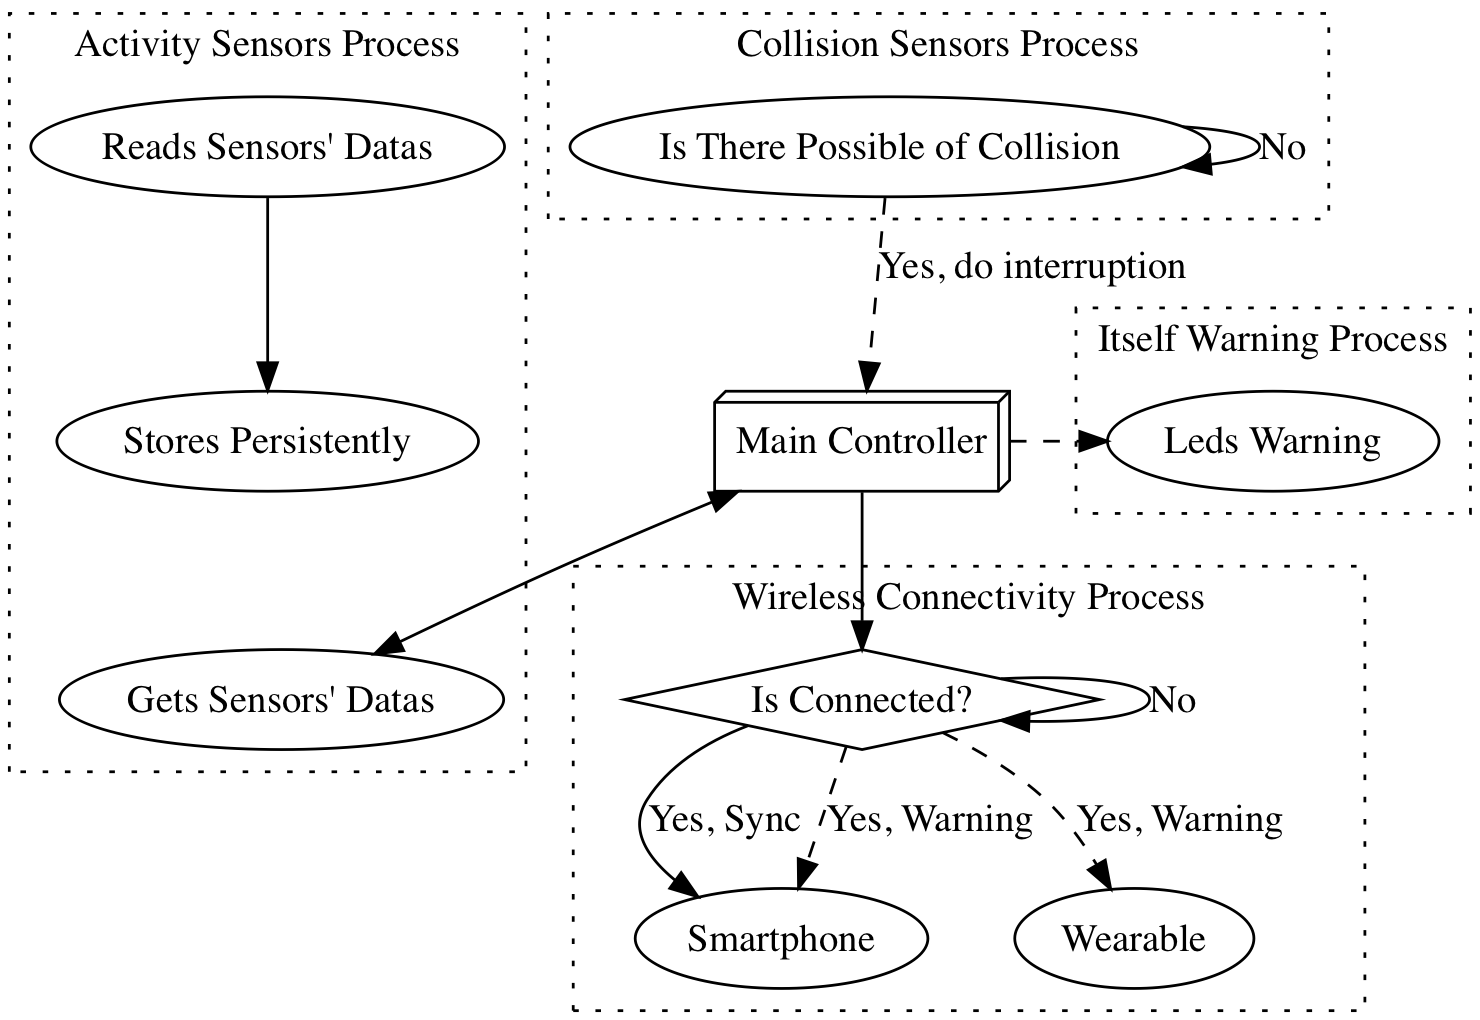
\includegraphics[width=0.9\textwidth]{img/graph_wearable2.png}
            \caption{Exemplificação de um grafo de chamada para o exemplo hipotético do capacete de segurança.}
            \label{fig:graph_w2}
         \end{figure}
         
         O grafo apresentado possui vários módulos que trabalham tanto colaborativamente quanto independente, e assim, serão mencionados e descritos separadamente a seguir para seu compreendimento.
         
         Antes de falar de cada módulo, será descrito alguns detalhes prévios.
         É possível visualizar que existem dois tipos de setas presente no grafo, isso foi feito como forma de demonstração de barramentos de comunicação na qual constituem de dados de baixa prioridade (troca de informações comuns) e dados com alta prioridade (interrupções).
         O primeiro, representado por uma seta não-tracejada ($\longrightarrow$) indica informações com baixa e o tracejado ($\dashrightarrow$), informações de alta prioridade, respectivamente.
         
         \begin{description}           
            
            \item [Sensores de Atividade:]
               Este bloco possui duas funções diferentes sendo a primeira apresenta neste tópico.
               O procedimento de leitura e armazenamento de dados sensoriais não é dependente do controlador, e com isso o processo (executado pelos procedimentos \texttt{lê sensores} e \texttt{Armazena Persistentemente}) é executado por si só.
               Dessa forma, neste processo, o capacete coleta dados e salva-os em memória constantemente a fim de criar um banco temporal de informações sem depender de um controlador para esta ação;              
               
            \item [Leitura de Dados \textit{Fitness} e Sincronização destes com o \textit{Smartphone}:]
               O outro processo, ainda relacionado ao modo anterior, parte da leitura dos dados já obtidos e envio desses do capacete para um aplicativo situado em um \textit{smartphone}.
               Este processo é já necessita de ser controlado por uma controladora e assim, foi associado com o controlador principal do projeto, para gerenciar com corretude a troca de informações;
               
            \item [Sensor de Colisão:]
               Com a leitura de dados sensoriais, outro processo também independente e de grande importância para o sistema é na análise de situações de risco e a geração de interrupções no controlador, caso exista uma.
               Esse módulo de sensoriamento de colisão compõe-se de procedimentos que realizam análises constantes de situações de risco do ciclista e enviando mensagens com interrupções para o controlador quando necessário;
               
            
            \item [Alarmes:] 
               Ao receber uma interrupção de colisão, o controlador fará logo em seguida os procedimentos de avisos nos respectivos dispositivos associados ao capacete no momento ocorrido.
               Dessa, forma o projeto constitui-se de dois tipos de avisos diferentes para o usuário, descritos a seguir:
               
               \begin{itemize}
                  \item \textbf{\textit{Alertas para Dispositivos Sem-Fio:}} 
                     Como o sistema possui comunicação sem-fio, é possível que ele envie um aviso de alerta para outros sistemas próximos a ele como \textit{smartphone} e \textit{wearables}.
                     Dessa forma, é possível que o \textit{smartphone} faça ações como vibrações ou sinais sonoros, bem como o \textit{wearable} e suas funções, a fim de alertar o usuário.
                  
                  \item \textbf{\textit{Alertas Próprio:}} 
                     Caso a comunicação não funcione, o dispositivo também terá acoplado a ele um sistema próprio na qual realizará o papel de informar o usuário sobre sua situação de risco. 
                     Este funcionará independente dos sistemas externos como meio alternativo de concluir o objetivo de informar o usuário imediatamente.
                     
               \end{itemize}
         \end{description}
         
         Com as informações obtidas até o presente momento por meio do \profile\ e o formato e fluxo do grafo, é possível identificar possíveis componentes a serem analisados em execução em \hardware, ou seja candidatos.
         
         Não é possível descrever os candidatos no exemplo hipotético pois necessita-se de informações de execução obtidas pelo \profile.
         Entretanto, podemos inferir uma lista de acordo com o propósito final de projeto e esta indução será descrita a seguir.
         Para um projeto que tenha como foco sua performance e confiabilidade, procedimentos como Verificação de Colisão e Leitura de Sensores de Atividade poderiam ser taxados como candidatos pelo fato de talvez estes se beneficiarem com a utilização de recursos em \hardware\ para a obtenção de seus objetivos.
         O procedimento de aviso integrado ao capacete também seria um candidato à análise, visto que desenvolvendo um circuito digital para seu acionamento, tem-se então respostas imediatas às interrupções geradas.
         Estes formam os componentes candidatos ao particionamento, segundo a análise induzida realizada.
         
         Por outro lado, o capacete também tem módulo de conexão sem-fio, requerendo um controlador para seu gerenciamento.
         Tal controlador deve ser capaz de certificar a conexão de dispositivos compatíveis de forma segura, realizar a transferência de informações de atividades entre o capacete e o aplicativo e tratar as interrupções com prioridade, sempre visando o consumo eficiente de energia.
         Estes, por sua vez, poderiam continuar em sua implementação em \software\ (não tornando candidatos), por se tratarem de procedimentos que não necessitam de performance, nem de grandes recursos de \hardware\ para a conclusão de suas tarefas.
         Os procedimentos compõe principalmente de leitura de dados em memória e seu envio via interface de comunicação sem-fio além do acionamento de tarefas a partir sinais interruptores.
         
         
       
      \paragraph{Análises de Síntese}
         Procedimento idêntico ao realizado com o \wearable\ hipotético da Seção~\ref{sec:hip1}.
         
         
      \paragraph{\textit{Solver}}
         Procedimento também idêntico ao realizado com o \wearable\ hipotético da Seção~\ref{sec:hip1}.
      
      
      
   \section{\Wearable\ Hipotético 3: Capacete Sensorial} \label{sec:hip3}

      \paragraph{Apresentação}
         Suponha uma outra situação na qual uma empresa que realiza o plantio e colheita de uma determinada fruta, necessita de acompanhar o clima e vários outros dados do ambiente em vários pontos diferentes de seus hectares.
         Entretanto, a instalação de postes coletores de dados nos seus vastos terrenos seriam um projeto inviável, segundo a empresa.
         
         
         % tipos de dados requeridos
         Feita a respectiva análise de requisitos do projeto, verificou-se que a empresa necessita de informações de: temperatura, pressão, radiação ultravioleta, chuva, luminosidade, fogo, radiação infravermelha, monóxido de carbono, gás natural, gás combustível, além de um sensor de distância em relação ao ponto atual do usuário.
         %Sensores passivos
         Dessa forma, foi apresentado então uma solução que baseia-se em um capacete com realidade virtual na qual realizaria a coleta dos dados por meio de sensores e, além de exibi-los à tela integrada nele, também enviaria-os para uma nuvem na qual apresentaria os dados para a central de processamento final.
         %Sensores ativos
         Diferentemente dos sensores passivos\footnote{Sensores na qual interpretam os respectivos dados do ambiente de forma passiva.} como sensor de temperatura, chuva e outros, o cálculo da distância partiria de um processo mais complexo, envolvendo várias fases de processamento.
         O procedimento, de modo introdutório, baseia-se na utilização de dois raios lasers junto à uma câmera externa para avaliar a distância de objetos.
         O vão entre os dois pontos é relativo à superfície do objeto, na qual altera de acordo com a distância entre o usuário e o objeto.
         Dessa forma, A distância entre os dois pontos aumenta na imagem captada à medida que a distância entre o usuário e o objeto reduz, e vice-versa.

         Assim, o Algoritmo~\ref{alg:wearable3_sensors} retrata, de forma geral, o processo de leitura dos sensores inclusive no cálculo de distância utilizando os lasers.
         Já o Algoritmo~\ref{alg:wearable3_main} gerencia os processos de leitura, exibição dos dados na tela do dispositivo e também o envio deste para a nuvem.
   
         \begin{algorithm}[h]
            \SetKwProg{Fn}{Function}{ do}{end}
            \SetKwData{md}{vector\_data}
            \SetKwFunction{stemp}{reads\_temperature}
            \SetKwFunction{spressure}{reads\_pressure}
            \SetKwFunction{suv}{reads\_ultraviolet}
            \SetKwFunction{srain}{reads\_rain}
            \SetKwFunction{sluminosity}{reads\_luminosity}
            \SetKwFunction{sfire}{reads\_fire}
            \SetKwFunction{sir}{reads\_infrared}
            \SetKwFunction{scarbon}{reads\_carbon\_monoxide}
            \SetKwFunction{snaturalgas}{reads\_natural\_gas}
            \SetKwFunction{sgas}{reads\_gas}
            \SetKwFunction{sdistance}{reads\_distance}
            \SetKwFunction{img}{image\_process}

            \BlankLine
            \KwOut{data's sensors vector.}
            \BlankLine

            \Fn{reads\_sensors}{
               \BlankLine
               \tcp{statements}
               \md\tcp*{data's vector}
               \BlankLine
               \tcp{reads passive sensors}
               \md $\leftarrow$ \stemp{}\;
               \md $\leftarrow$ \spressure{}\;
               \md $\leftarrow$ \suv{}\;
               \md $\leftarrow$ \srain{}\;
               \md $\leftarrow$ \sluminosity{}\;
               \md $\leftarrow$ \sfire{}\;
               \md $\leftarrow$ \sir{}\;
               \md $\leftarrow$ \scarbon{}\;
               \md $\leftarrow$ \snaturalgas{}\;
               \md $\leftarrow$ \sgas{}\;
               \BlankLine
               \tcp{reads active sensors}
               \md $\leftarrow$ \sdistance{\img{}}\;
               
               \BlankLine
               \Return \md\tcp*{return the datas to the controller}
            } 

            \caption{\Wearable\ 3 - Procedimentos de leitura do ambiente por meio de uma estação de sensores.}
            \label{alg:wearable3_sensors}
         \end{algorithm}
                  
         
         \begin{algorithm}[H]
            \SetKwData{md}{vector\_data}
            \SetKwData{sx}{sensor$_i$}
            \SetKwFunction{leSensores}{reads\_sensors}
            \SetKwFunction{preprocess}{pre\_process}
            \SetKwFunction{process}{processes}
            \SetKwFunction{atuacao}{operates}
            \SetKwFunction{bu}{cloud\_backup}
            \SetKwFunction{showit}{show\_informations}

            \BlankLine
            \KwOut{acting.}
            \BlankLine

            \Begin{
               \BlankLine
               \tcp{statements}
               \md\tcp*{data's vector}
               \BlankLine

               \While{wearable mode on}{
                  \md $\leftarrow$ \leSensores{}\;

                  \BlankLine

                  \showit{\md}\tcp*{shows the datas on the wearable's screen}

                  \BlankLine
                  \bu{\md}\tcp*{saves the data persistently}
                  
                  \BlankLine
               }
            }

            \caption{\Wearable\ 3 - Método principal para controle.}
            \label{alg:wearable3_main}
         \end{algorithm}


      
      \paragraph{Análise Usando \Profile}
      
         Com o processo de análise pela técnica de \profile\ é possível identificar os principais procedimentos que requerem o maior tempo de processamento.
         Procedimento semelhante às análises de \wearables\ anteriores (Seções~\ref{sec:hip1} e \ref{sec:hip2}).
         
         O método de cálculo de distância utiliza de vários procedimentos complexos, possuindo talvez a maior quantidade de recursos de processamento e tempo para a conclusão de suas tarefas.
         Com o processo de geração de código HDL por meio de HSL, seria possível utilizar de recursos como aceleradores para o processamento de imagem a fim de agilizar o processamento ou a redução de gasto energético, por exemplo.


      \paragraph{Grafo}
         O grafo representante do Algoritmo~\ref{alg:wearable3_sensors} é exibido na Figura~\ref{fig:graph_w3_a}.
         É apresentado o processo de captura de dados pelos sensores passivos e também o método de cálculo de distância por meio dos dos lasers.
         Ao lado direito do grafo, existe um ponto na qual aponta para o processo de leitura dos sensores.
         Tal ponto representa a invocação do método, ou seja, os dados dos sensores só serão lidos quando forem solicitados e assim, serão retornados como é exibido pelo segundo ponto a baixo do grafo.
         
         Realizado uma invocação do método de leitura de sensores, os dados de cada sensor passivo serão lidos e armazenados num vetor de informações.
         Por outro lado, também é realizado a captura de imagens para processamento da distância na qual o processo consiste, de forma geral, em três etapas, sendo elas a captura e o processamento da imagem e o cálculo da distância em relação à distância dos pontos.
        
         \begin{figure}[h] \centering
            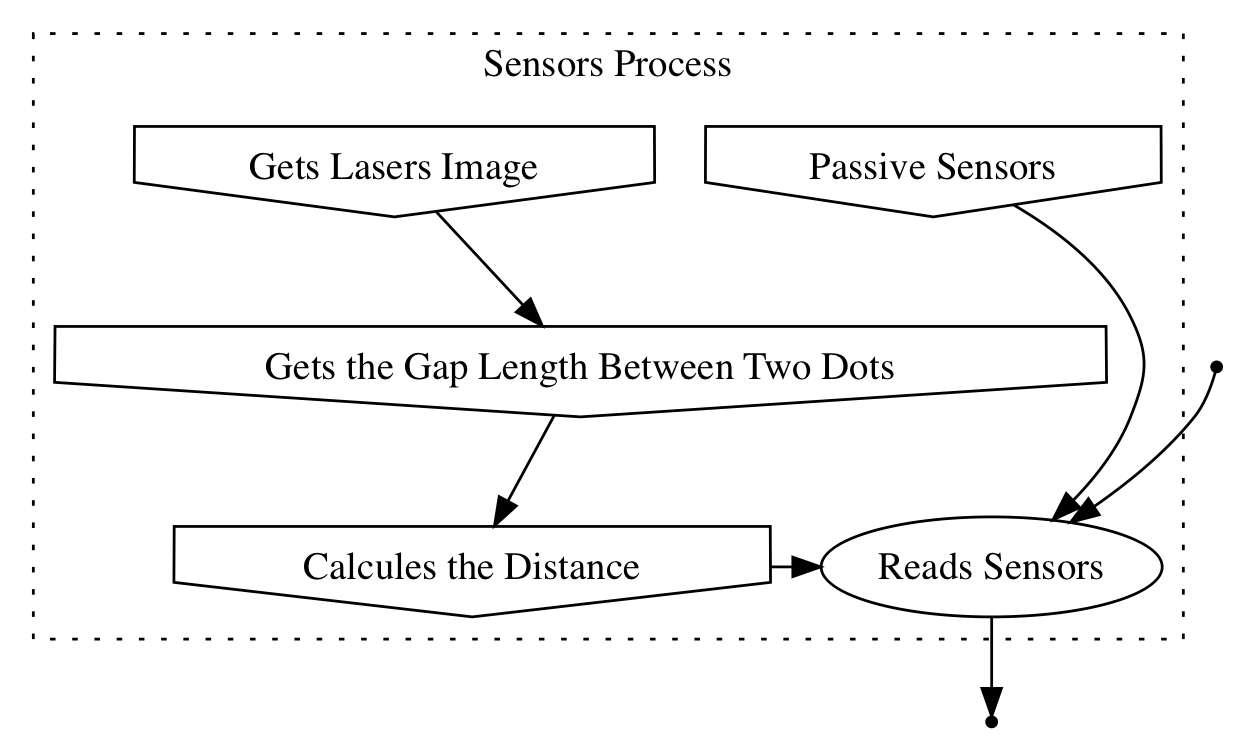
\includegraphics[width=0.8\textwidth]{img/graph_wearable3_b.png}
            \caption{Exemplificação de um grafo de chamada para o exemplo.}
            \label{fig:graph_w3_a}
         \end{figure}
         
         Já o Algoritmo~\ref{alg:wearable3_main} é representado pelo grafo da Figura~\ref{fig:graph_w3_b}.
         Constitui-se do processo principal na qual invoca o procedimento de leitura de sensores.
         Como este é basicamente para controle, nele ordena-se os passos de leitura, exibição e envio dos dados para uma nuvem, caso o dispositivo permaneça ligado neste processo.
         O módulo de leitura de sensores exibido no canto esquerdo da Figura~\ref{fig:graph_w3_b} simplifica o processo da Figura~\ref{fig:graph_w3_a}, já explicada.
         
         \begin{figure}[h] \centering
            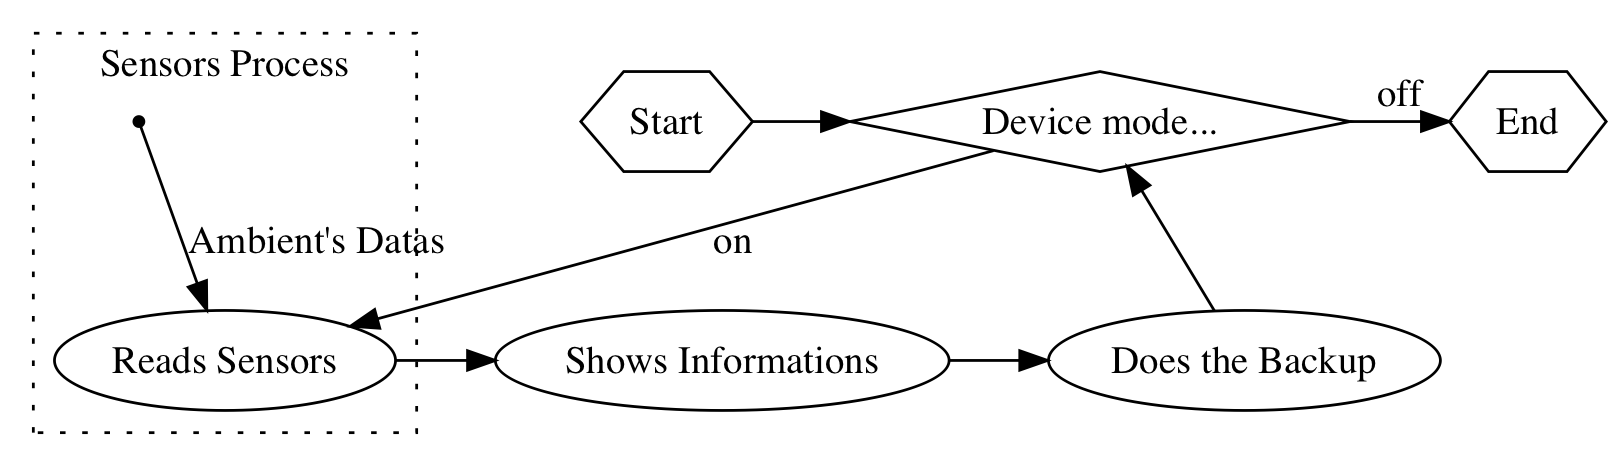
\includegraphics[width=1\textwidth]{img/graph_wearable3.png}
            \caption{Exemplificação de um grafo de chamada para o exemplo.}
            \label{fig:graph_w3_b}
         \end{figure}
         

      \paragraph{Análises de Síntese}
         Idem ao processo das seções anteriores, na qual realiza uma visão do projeto com os candidatos apresentados pelas ferramentas e sintetiza-os a fim de avaliar suas características de funcionamento.
         
      \paragraph{\textit{Solver}}
         Idem às análises anteriores (Seções~\ref{sec:hip1} e \ref{sec:hip2}).

   
   
   
   
   
   
   
   
   
   
	%%\input{tex/chap-Resultados.tex}
	%!TEX root = ../main_text.tex
%\chapter{Experimentos e Resultados} \label{chap:experimentos}

\chapter{Conclusões Parciais e Trabalho Futuro} \label{chap:conclusao}

   Neste capítulo serão descritas as conclusões parciais da pesquisa realizada até o momento e as próximas etapas a serem executadas.   

   \section{Conclusões}
      %demora da pesquisa em wearables
      Mesmo a tecnologia embarcada tenha tido um grande avanço nos últimos tempos sendo utilizada nos mais diversos fins, sistemas \wearables\ tiveram seu primeiro aparecimento em pesquisas científicas em \citeyear{Mann1996} por \citeauthor{Mann1996}.
      Isso, por causa de empecilhos tecnológicos e ferramentais como a necessidade da miniaturização, mobilidade e eficiência energética da tecnologia dos equipamentos utilizados na qual, sem tais especificações, seria inviável a utilização do \wearable.
      
      %não tem particionamento para wearables
      Existe várias pesquisas relacionadas à área de sistemas embarcados no âmbito de particionamento de \hs, inclusive utilizando FPGAs como meio.
      Entretanto, até o momento deste, não foi encontrado nenhum relato de experiências científicas sobre o particionamento para sistemas \wearables\ com utilização de recursos de \hardwares\ reconfiguráveis, tema tratado neste documento.
      
      % objetivos concluídos até então
      Objetivos realizados até o presente momento:
      
      \begin{itemize}
         \item Introdução de sistemas computacionais \wearables\ e apresentação do problema de particionamento \hs\ no âmbito de de sistemas computacionais embutidos, com foco em sistemas \wearables;
         
         \item Apresentação de:
         \begin{itemize}
            \item Principais soluções apresentadas ao logo dos anos e as utilizadas atualmente;
            \item Ferramentas HLS como LegUp e OpenCL para a geração de sistemas computacionais que usufruem de aceleradores em \hardware.
         \end{itemize}
         
         \item Apresentação da abordagem metodológica a ser utilizada para a procura da solução do problema de particionamento \hs\ apresentado.
      \end{itemize}
      
      
   \section{Trabalho Futuro}
      A seguir será apresentado os tópicos relativos às próximas etapas a serem realizadas neste trabalho.
      
      \begin{itemize}
         \item Geração de HDL, utilizando as ferramentas automatizadas quando aplicável:
         \begin{itemize}
            \item LegUp;
            \item OpenCL.
         \end{itemize}
         
      \item Realizar-se-á análises de algoritmos situados em sistemas diferentes, sendo esses:
         \begin{itemize}
            \item \textbf{Totalmente em nível de \software:} sem auxílio de qualquer acelerador como ao utilizar a plataforma Beagle Bone como sendo o sistema embarcado completo para execução em aplicações \wearables; e em
            
            \item \textbf{Híbridos:} formados de processadores e aceleradores utilizando dos recursos de dispositivos reconfiguráveis  a fim de prover maior \speedup\ utilizando recursos de \hardware.
         \end{itemize}
         
         \item A análise de desempenho será feita com os dados obtidos dos dois sistemas citados acima.
         Executando o projeto nos dois sistemas, em nível de \software\ e híbrido, é possível relacionar o ganho de desempenho realizando as operações apresentadas na Seção~\ref{sec:ganho_performance}.
                  
         
      	\item Redução do tempo de seu desenvolvimento até a disposição do produto ao mercado utilizando os recursos que o desenvolvimento com \hardware\ reconfigurável proporciona. %Wolf1994.
         \end{itemize}
      
\end{mainmatter}

%% Produce the appendices
\begin{appendices}
\begin{flushleft}

\end{flushleft}
	\selectlanguage{brazilian}
  	%%!TEX root = ../main_text.tex

\chapter{Apêndices}


\begin{algorithm}[h] \footnotesize
    \KwIn{vetor buffer.}
    \KwOut{média, variância, desvio padrão.}
    
    \BlankLine
    \Begin{
        $\vars{soma}= \vars{variancia} = 0$;
        \BlankLine
        
        \lFor{$\func{length}(\vars{buffer})$}{$\vars{soma} \mathrel{+}= \vars{buffer}_i$}
        \BlankLine
        
        $\vars{media} = \vars{soma} \div \func{length}(\vars{buffer})$\;
        \BlankLine
        
        
        \lFor{$\func{length}(\vars{buffer})$}{
            $\vars{variancia} \mathrel{+}= (\vars{buffer}_i - \vars{media})^2$
        }
        
        \BlankLine
        $\vars{variancia} \mathrel{\div}= \func{length}(\vars{buffer})$\;
        \BlankLine
        $\vars{dp} = \func{sqrt}(\vars{variancia})$\;
        
        \Return \vars{media}, \vars{variancia}, \vars{dp}\;
    }
    \caption{Método Estatístico.}
    \label{alg:statistic}
\end{algorithm}

\begin{algorithm}[h] \footnotesize
    \KwIn{vetor buffer, ponto.}
    \KwOut{distância interpolada.}
    
    \BlankLine
    \Begin{
        
        $\vars{nova\_distancia} = 0$\;
        \BlankLine
        
        \For{$\vars{i}\ in\ 1:\func{length}(\vars{buffer})$}{
            $\vars{c} = \vars{d} = 1$;
            
            \BlankLine
            \For{$\vars{j}\ in\ 1:\func{length}(\vars{buffer})$}{
                \If{$\vars{i} \ne \vars{j}$}{
                    $\vars{c} \mathrel{\times}= \vars{ponto} - \vars{j}$;
                    %\BlankLine
                    $\vars{d} \mathrel{\times}= \vars{i} - \vars{j}$;
                }
            }
            \BlankLine
            $\vars{nova\_distancia} \mathrel{+}= \vars{buffer}_i \times \vars{c} \div \vars{d}$;
        }
        \BlankLine
        
        \lIf{$\vars{nova\_distancia} \ge 0$}{$\Return\ \vars{nova\_distancia}$}
        \lElse{$\Return\ 0$}
        
    }
    \caption{Método Interpolação por Lagrange.}
    \label{alg:lagrange}
\end{algorithm}

\begin{algorithm}[h] \footnotesize
    \KwIn{distância$_1$, distância$_2 = 0$, distância$_3 = 0$.}
    \KwOut{primaridade.}
    
    \BlankLine
    \Begin{
        
        $\vars{primo} = \vars{distancia}_1 + \vars{distancia}_2 + \vars{distancia}_3$;
        \BlankLine
        
        \lIf{$\vars{primo} \le 1$}{\Return 0}
        \BlankLine
        \lIf{$\vars{primo} = 2$}{\Return 1}
        \BlankLine
        
        \lIf{\vars{primo} $\func{mod}(2) = 0$}{$\vars{primo} \mathrel{+}= 1$}
        \BlankLine
        
        $\vars{divisor} = \vars{primo} \div 2$;
        
        \lIf{\vars{divisor} $\func{mod}(2) = 0$}{$\vars{divisor} \mathrel{+}= 1$}
        \BlankLine
        
        
        \While{\vars{divisor} $> 2$}{
            \lIf{\vars{primo} $\func{mod}(divisor) = 0$}{\Return 0}
            \BlankLine
            \lElse{\vars{divisor} $\mathrel{-}= 2$;}
            
        }
        \Return 1;
        
    }
    \caption{Método Número Primo.}
    \label{alg:prime}
\end{algorithm}

\begin{algorithm}[h]
    \footnotesize
    \KwIn{distância lida; distância mínima.}
    \KwOut{boolean.}
    
    \BlankLine
    \Begin{
        \tcp{Se há risco, retorna TRUE}
        \uIf{\vars{distancia\_lida} $\le$ \vars{distancia\_minima}}{
            \Return 1
        }
        \lElse {
            \Return 0
        }
        
    }
    \caption{Método avaliação de Risco.}
    \label{alg:risk}
\end{algorithm}

%%!TEX root = ../main.tex
% !TeX encoding = UTF-8

       \begin{algorithm}[t] \footnotesize
           \KwIn{vetor buffer.}
           \KwOut{média, variância, desvio padrão.}
           
           \BlankLine
           \Begin{
               $\vars{soma}= \vars{variancia} = 0$;
               \BlankLine
               
               \lFor{$\func{length}(\vars{buffer})$}{$\vars{soma} \mathrel{+}= \vars{buffer}_i$}
               \BlankLine
               
               $\vars{media} = \vars{soma} \div \func{length}(\vars{buffer})$\;
               \BlankLine
               
               
               \lFor{$\func{length}(\vars{buffer})$}{
                   $\vars{variancia} \mathrel{+}= (\vars{buffer}_i - \vars{media})^2$
               }
               
               \BlankLine
               $\vars{variancia} \mathrel{\div}= \func{length}(\vars{buffer})$\;
               \BlankLine
               $\vars{dp} = \func{sqrt}(\vars{variancia})$\;
               
               \Return \vars{media}, \vars{variancia}, \vars{dp}\;
           }
           \caption{Método Estatístico.}
           \label{alg:statistic}
       \end{algorithm}
       
       \begin{algorithm}[t] \footnotesize
           \KwIn{vetor buffer, ponto.}
           \KwOut{distância interpolada.}
           
           \BlankLine
           \Begin{
               
               $\vars{nova\_distancia} = 0$\;
               \BlankLine
               
               \For{$\vars{i}\ in\ 1:\func{length}(\vars{buffer})$}{
                   $\vars{c} = \vars{d} = 1$;
                   
                   \BlankLine
                   \For{$\vars{j}\ in\ 1:\func{length}(\vars{buffer})$}{
                       \If{$\vars{i} \ne \vars{j}$}{
                           $\vars{c} \mathrel{\times}= \vars{ponto} - \vars{j}$;
                           %\BlankLine
                           $\vars{d} \mathrel{\times}= \vars{i} - \vars{j}$;
                       }
                   }
                   \BlankLine
                   $\vars{nova\_distancia} \mathrel{+}= \vars{buffer}_i \times \vars{c} \div \vars{d}$;
               }
               \BlankLine
               
               \lIf{$\vars{nova\_distancia} \ge 0$}{$\Return\ \vars{nova\_distancia}$}
               \lElse{$\Return\ 0$}
               
           }
           \caption{Método Interpolação por Lagrange.}
           \label{alg:lagrange}
       \end{algorithm}
       
       \begin{algorithm}[t] \footnotesize
           \KwIn{distância$_1$, distância$_2 = 0$, distância$_3 = 0$.}
           \KwOut{primaridade.}
           
           \BlankLine
           \Begin{
               
               $\vars{primo} = \vars{distancia}_1 + \vars{distancia}_2 + \vars{distancia}_3$;
               \BlankLine
               
               \lIf{$\vars{primo} \le 1$}{\Return 0}
               \BlankLine
               \lIf{$\vars{primo} = 2$}{\Return 1}
               \BlankLine
               
               \lIf{\vars{primo} $\func{mod}(2) = 0$}{$\vars{primo} \mathrel{+}= 1$}
               \BlankLine
               
               $\vars{divisor} = \vars{primo} \div 2$;
               
               \lIf{\vars{divisor} $\func{mod}(2) = 0$}{$\vars{divisor} \mathrel{+}= 1$}
               \BlankLine
               
               
               \While{\vars{divisor} $> 2$}{
                   \lIf{\vars{primo} $\func{mod}(divisor) = 0$}{\Return 0}
                   \BlankLine
                   \lElse{\vars{divisor} $\mathrel{-}= 2$;}
                   
               }
               \Return 1;
               
           }
           \caption{Método Número Primo.}
           \label{alg:prime}
       \end{algorithm}
       
       \begin{algorithm}[t]
           \footnotesize
           \KwIn{distância lida; distância mínima.}
           \KwOut{boolean.}
           
           \BlankLine
           \Begin{
               \tcp{Se há risco, retorna TRUE}
               \uIf{\vars{distancia\_lida} $\le$ \vars{distancia\_minima}}{
                   \Return 1
               }
               \lElse {
                   \Return 0
               }
               
           }
           \caption{Método avaliação de Risco.}
           \label{alg:risk}
       \end{algorithm}
       


\begin{comment}
Por exemplo, considerando as vogais da língua inglesa onde o universo $ U = \{a, e, i, o, u, y\} $. 
Assim, uma partição desse problema $ \mathcal{X}_a $ de $ U $ pode ser representado por


\begin{equation}
\mathcal{X}_a = \left\{\{a, e, i, o, u\}, \{y\}\right\} \label{eq:xa}
\end{equation}

e supondo que o conjunto pode ser representando por cada unidade, uma outra forma de representação pode ser


\begin{eqnarray}
\mathcal{X}_b &=& \left\{\{a\}, \{e\}, \{i\}, \{o\}, \{u\}, \{y\}\right\}
\end{eqnarray}

Sobre tais conceitos, a Partição \ref{eq:part_c} viola a Equação \ref{eq:part_form_1} e a Partição \ref{eq:part_d} viola as Equações \ref{eq:part_form_2} e \ref{eq:part_form_3}.

\begin{eqnarray}
\mathcal{X}_c &=& \left\{\{a\}, \{e\}, \{i\}, \{o\} \right\} \label{eq:part_c} \\
\mathcal{X}_d &=& \left\{\{a, e, i\}, \{i, o, u, y\}, \{\}\right\} \label{eq:part_d}
\end{eqnarray}

A Figura \ref{fig:f4-2} ilustra o $ \mathcal{X}_a $ graficamente, segundo a Partição \ref{eq:xa}.

\begin{figure}[h] \centering
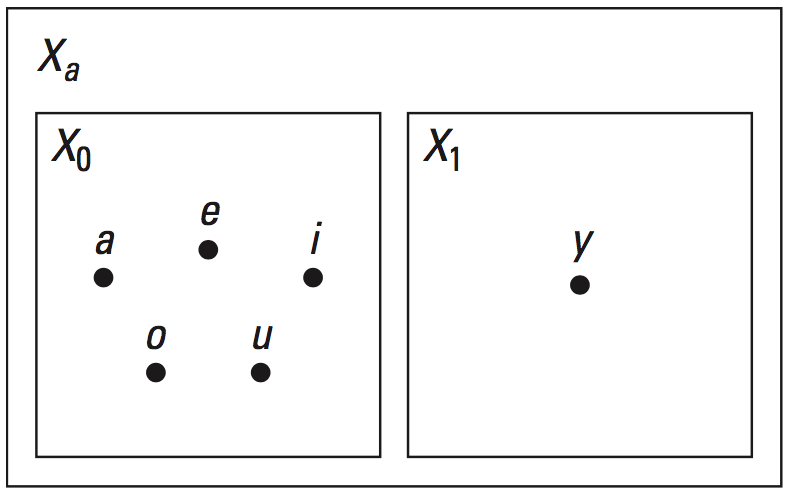
\includegraphics[width=0.5\textwidth]{img/f4-2.png}
\caption{Figura representativa do mapeamento da aplicação.}
\label{fig:f4-2}
\end{figure}
\end{comment}

\begin{comment}

%\chapter{Transferência de Estado} 

\section{Transferência de Estado} \label{chap:tranferencia}
   Segundo \citeauthor{Sass2010}, manter estado consistente sobre dispositivos FPGA e processadores é um desafio.
   Isso pois, como cada FPGA tem sua própria hierarquia de memória independente, estados são amplamente distribuídos no \design\ e há ampla variedade de interconexões entre FPGA e processadores.
   Assim, isso significa menos estados para serem transferidos e grande variedade de mecanismos disponíveis.
   Os tipos de estados serão descritos a seguir pois são requisitos para identificação de qual parte do estado da aplicação precisa ser explicitada pela comunicação processador e recurso.
   %Para entender melhor deve-se definir dois conceitos sendo eles estado afetado e preso ajudando a decidir quais partes do estado da aplicação necessitam de ser explicitamente comunicados entre processador e recurso.
   
   \begin{description}
      \item [Estado Afetado:]
      Na computação alguns estados são independentes pela construção e não precisam de ser transferidos de lugares. Retirando tais estados, restam os estados afetados.
      
      Esses, são os dados da aplicação que, durante a transferência de controle, podem ser modificados ou lidos por um recurso ou processador, necessitando de ser consistente entre todas as distribuições.
      %Estados afetados podem existir em grande escala. Principalmente quando arranjos, estruturas de dados complexas ou ponteiro estão envolvida e podem ser acessados de várias formas possíveis e geralmente não é possível saber se dois ponteiros estão apontando para um mesmo endereço.
      
      \item [Estado Preso:]
      Acontece quando parte da hierarquia de memória é compartilhada, nem todo o dado tem que ser explicitamente transferido e assim, caso todo o estado corrente esteja em memória primária (RAM) e ambos os dispositivos possuem acesso a ela, então não existe razão para a transferência explícita dos dados.
      
      Processadores modernos são construídos com quantidade significativa de memória que podem ser utilizadas como parte de estado sem a atualização da memória primária.
      Compiladores naturalmente utilizam toda a vantagem de registradores para armazenar os estados.
      
      Implementações em \hardware\ também incorporam dados ao longo do projeto e seus registradores e \textit{flip-flops} possuem valores intermediários entre ciclos de \textit{clock} dentro do projeto.
      O estado de uma aplicação é armazenado em várias partes do sistema.
      Para um recurso implementar parte de uma aplicação, precisa-se então integrar-se com parte do estado.
      
      Esse pode ser considerado mais facilitado pelo fato de que o estado está localizado em um espaço comum. Mas se um estado está localizado num registrador ou em uma cache de um processador, ele não pode ser acessado pelo sistema externo e, neste caso, o estado encontra-se preso e deve ser explicitamente transmitido pela interface.
      
      \begin{figure}[h] \centering
         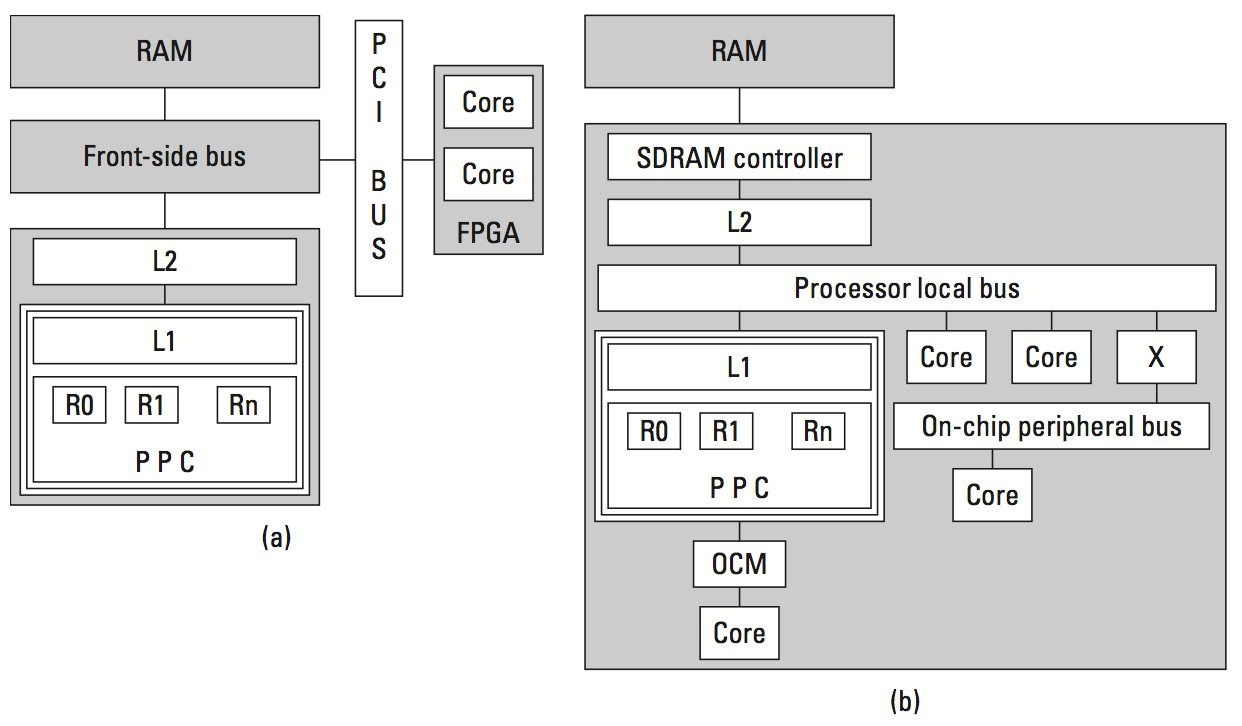
\includegraphics[width=1\textwidth]{img/f4-7.png}
         \caption{Situações na qual pode ocorrer bloqueio de estado. \textit{a)} Situação na qual existe um processador externo ao FPGA e sua memória interna é inacessível. \textit{b)} Situação onde o processador situa-se na plataforma FPGA. Fonte: \citet{Sass2010}.}
         \label{fig:4-7}
      \end{figure}
      
      Em ambos os casos mostrados na Figura \ref{fig:4-7} o FPGA (representado pelos \cores\ não possui autorização para o acesso aos registradores do processador (representados por $R_n$). Mesmo em \textit{b)} onde o processador é integrado à plataforma FPGA, não possui-se acesso sendo necessário a disponibilização manual deste.
   \end{description}
   
   
   \section{Problema de Transferência de Estado}
   Estados afetados que estão presos necessitam de ser explicitamente comunicados e esta é feita por um processo chamado \textit{marshaling}.
   Assim, será feito um \textit{Marshaling} de grupos de elementos de um estado afetado de uma aplicação em registros lógicos que são explicitamente transferidos.
   
   Tendo a premissa que o processador possui o controle inicial, tem-se quatro tipos de registros que podem ser utilizados.
   Os dois primeiros, \textit{Type-I} e \textit{Type-F}, são utilizados para iniciar e outro para finalizar a transferência de um conjunto de elementos para o recurso, respectivamente.
   Os outros dois tipos de \textit{marshal} são usados repetidamente. Um quando o recurso é invocado (\textit{Type-CI}, do inglês \textit{copy-in}), e quando é completado (\textit{Type-CO}, do inglês \textit{copy-out}).
   %Um exemplo de \textit{Type-F} é quando tem-se um \core\ que acumula um valor em uma variável global. O registro \textit{Type-F} seria utilizado para ler o valor da variável após sua última invocação.
   
   Um processo de tradução pode ser incorporado com o \textit{marshaling}, sendo o exemplo a conversão de ponto flutuante para fixo quando transferido para um recurso o que acontece também com transformações mais complexas.
   %O agrupamento de elementos é lógico pelo fato do \textit{assembly} não significar estritamente que os elementos são copiados para uma memória de locação contínua.
   
   A forma mais simples de transferir estados é copiando os registros, parando o processador enquanto o recuso processa.
   Este é chamado de \textit{push} os dados no qual transmite o dado antes da transferência do controle. Ao final, realiza-se o \textit{pulls} dos dados.
   
   
   Embora isso, uma transferência instantânea de estado não é sempre simples. Quando o estado afetado é grande mas o dado atua é pequeno, o padrão de acesso ao dado é randômico e a transferência lógica de registro é larga sendo mais vantajoso o uso de interfaces de comunicação para servir o recurso. Ou seja, utilizado quando o recurso foi designado para reduzir a latência da tarefa e a transferência do registo é pequena.
   Quando o registro lógico e o dado atual são largos, utiliza-se de padrão de acesso regula que transmite dados continuamente. É usado quando o recurso aumenta o \textit{throughput} e a redução de latência ou metas de performance não são possíveis.
   
   Isso é útil por exemplo na ordenação onde transferir um arranjo completo quando invocado é uma operação cara e desnecessária já que dependendo do algoritmo, pode-se utilizar apenas frações deste.



\section{Análise de Performance de Sistema} \label{sec:amdahl}
	A análise de performance de um sistema é definida pela Lei de \citeauthor{amdahl1967validity} de \citeyear{amdahl1967validity} relaciona o tempo gasto para executar uma tarefa com um único processador e o gasto com $j$ processadores. Nessa definição, $T_1$ representa um computador sequencial e $T_j$ um computador com $j$ núcleos. Sendo $s$ a fração relativa ao trecho estritamente serial e $q$ a fração relativa ao tempo paralelizável, tem-se as seguintes definições básicas

	\begin{eqnarray}
		T_1   & = & s + q = 1\\
		T_j & = & T_1 \times s + T_1 \times  \left(\frac{q}{j}\right)
	\end{eqnarray}

    O \textit{speedup}, cálculo do ganho da utilização de vários \cores, é obtido pela Fórmula \ref{eq:spu_init}.

	\begin{eqnarray}
		Speedup & = & \frac{T_1}{T_j} \label{eq:spu_init}
	\end{eqnarray}

	Dessa forma, realizando substituições das definições básicas na Equação \ref{eq:spu_init}, tem-se a Equação final de \speedup\ em \ref{eq:spu_fim}.

	\begin{eqnarray}
		Speedup & = & \frac{T_1}{T_j} = \frac{(s + q)}{\left(s+\frac{q}{j}\right)} = \frac{1}{\left(s+\frac{q}{j}\right)} \\
		%T(n) & = & T(1)(B + \frac{1}{n}(1 - B)) \\
		Speedup & = & \frac{1}{s + \left(\frac{1 - s}{j}\right)} \label{eq:spu_fim}
	\end{eqnarray}

	Essa equação articula os limites de um melhoramento global para uma aplicação que um simples aprimoramento pode fazer em tempo de execução.

	Generalizando a equação para incluir todo potencial de aprimoramento e métricas de performance arbitrária, pode-se caracterizar os limites como coleções de aprimoramento.
    Se esses aprimoramentos são recursos de \hardware\ e podemos antecipar o ganho requerido ganho potencial de recursos para cada recurso, então pode-se desenvolver um modelo que irá orientar ao processo de particionamento.

    Tal lei não é adequada pois:
	\begin{itemize}
		\item Visa um simples realce e não nos auxilia a selecionar um subconjunto de uma coleção de recursos potenciais;
		\item Foca somente no tempo de execução;
		\item Não visa recursos requeridos;
		\item Não visa custo de comunicações.
	\end{itemize}

	Perfis baseados em exemplos requerem representações de entrada e é uma aproximação de tempo gasto. Sem implementar todo o potencial de recursos em \hardware, pode ser difícil antecipar os recursos requeridos. Pode-se com determinação analítica calcular quantos ciclos de \textit{clock} um recurso de \hardware\ irá tomar, podendo assim calcular métricas como \speedup. Entretanto, é impossível saber quando um processo arbitrário será completado. Ao invés de prover uma solução automatizada, a solução analítica simplesmente provê um \textit{framework} para guiar um \designer\ de sistema a criar uma solução criativa.

	\subsection{Abstração e Estado}
		No contexto de desenvolvimento, um módulo é uma abstração de alguma funcionalidade em um sistema.
		A palavra abstração é definida como `operação intelectual em que um objeto de reflexão é isolado de fatores que comumente lhe estão relacionados na realidade', ou seja, no sentido amplo da palavra, significa tirar fora, extrair, remover.
		Um módulo tenha uma boa abstração terá suas interfaces e descrições mais fáceis de serem compreendidas, entretanto isso torna sua implementação mais complexa.
		Uma boa abstração capta todas características importantes de algo criando assim uma organização e dessa forma, uma representação rica em informação pode não ser tão relevante\todo{rever}.
		Em contra partida, caso seja feito uma abstração ruim de algo, forçará-nos a pensar não só sobre a singularidade do módulo, mas também como foi implementado, o que não é uma informação valiosa para uma abstração.

		Estado é uma palavra já conhecida no âmbito de sistemas eletrônicos. Estados são explicitados num \design\ de máquinas sequenciais por exemplo, e podem ser um ponto de memória de dispositivos eletrônicos.
		Em sistemas embarcados, sua definição é um pouco mais abstrata à dita já que um estado de módulo pode ser armazenado em vários lugares em várias formas distintas como \textit{flip-flops}, \textit{static RAM}, arquivos, ou até mesmo em memórias \textit{off-chip}. Dessa forma, estado pode ser definido como uma condição de memória onde é possível segurar uma informação por um certo período de tempo.

	\subsection{Coesão e Acoplamento}
		Definido o conceito de abstração e estado de sub-rotinas, é necessário esclarecer os conceitos de mensurações sobre módulos sendo essas coesão e acoplamento.

		Coesão é uma métrica de abstração. Assim, se os detalhes dentro de um módulo no ato da implementação são funcionalidades compreendidas facilmente, então o módulo possui coesão.
		O acoplamento é a forma de como os módulos estão relacionados uns com os outros. Uma dependência entre módulos existe quando um comunica diretamente com outro. Quando um módulo \A\ invoca um módulo \B, então \A\ depende de \B. Entretanto, \B\ não necessariamente depende de \A.

		Dependências não são sempre explícitas e com isso entra-se o conceito de estado para auxiliar na formação de um módulo.
		Quando dois módulos parecem não ter nenhuma dependência entre si mas o sistema exige que ambos tenham terminado seus processamentos ao mesmo tempo, cria-se então uma dependência e etiquetados como dependentes por temporização. O fato de dois módulos serem utilizados no mesmo estado os tornam dependentes.

		São necessárias para que o procedimento possa funcionar corretamente com todos os outros módulos, mas precisa-se saber o grau de acoplamento em número e tipo.
		%Dependência surgidas a partir de interfaces formais possuem  são as melhores formas de dependências.
		Uma forma de reduzir acoplamento em sistemas são por meio de encapsulamentos. Eles envolvem manipulações de estado e introdução à interface formal sendo a ideia principal a movimentação de um estado dentro de um módulo e fazer com que isso seja exclusivo, ou seja, não compartilhado, técnica bastante eficaz. Pode ser reconhecida também como informação escondida.
		Ao realizar tal procedimento, permite-se maior liberdade de mudança interna no módulo pois, alterando seu estado, a mudança deste não introduz erro em outro módulo consequente. E se o módulo possuir uma boa abstração, então a informação escondida também permite que o módulo seja implementado de forma mais independente.

		É preciso evitar acoplamentos quando desnecessário e para isso existem várias técnicas para manipulação do grau de acoplamento. Uma fácil de ser resolvida é como exibida na Figura \ref{fig:acoplamento}. Em a) que os sub-módulos \B\ e \C\ possuem dependência do módulo somatório \A. Na Figura \ref{fig:acoplamento} b) o somatório \A\ é duplicado dentro de cada sub-módulo eliminando cada uma das dependências existentes, reduzindo o fator de acoplamento.

		\begin{figure}[h] \centering
			\includegraphics[width=0.6\textwidth]{img/f3-4.png}
			\caption{Exemplo de redução do fator acoplamento em um módulo.}
			\label{fig:acoplamento}
		\end{figure}

		%Será proposta uma situação exibindo o porquê desta abordagem pode ter mais vantagens: suponha que A foi designado para calcular somente números não-sinalizados. Mas com o passar do tempo, C necessita de operar com número sinalizados. Dessa forma, na Figura \todo{a} o \design\ deveria alterar tanto C quanto A. Alterando A, obrigatoriamente afetará B. Mesmo que B continue a trabalhar bem com a alteração de A, ouve uma cascata de alterações a serem feitas ao longo do tempo sobre algo que deveria ser pequeno, simples e isolado.

		%Discutindo sobre desvantagens deste procedimento, talvez se pensa que isso pode aumentar no tamanho do \design\ do projeto já que está duplicando um item, mas não. É possível que a funcionalidade de A seja simplesmente mesclado com o configurable logic block (CLB) já alocado para os sub-módulos B e C e consequentemente é possível que não haja nenhum ganho de conexão no CLB alocado. É claro que isso não é sempre verdade e é possível sim que tenha aumento de custo. Uma segunda desvantagem é, ao duplicar um módulo, agora se tem o mesmo componente em dois lugares. Se um erro for encontrado em um, deverá ser alterado noutro também.



\subsection{Invocação e Coordenação}

	Da mesma forma que modelos de computação sequencial e \textit{multithread} podem realizar invocações de sub-rotinas, o mesmo pode ser realizado em \hardware\ com o codinome de política de coordenação. Em nível de \hardware\ existe diferenciações pois neste não existe controle de de \textit{thread} mas geralmente possui somente um controlador que habilita ou não o recurso para processamento. Muitas máquinas de estado têm uma ordem de estados \textit{idle} e a transferência de controle pode ser a sua ativação. Existe três abordagens para coordenar um \hardware\ e \textit{\software} e serão descritas a seguir.


	\subsubsection{Modelo de Coprocessador}

		Também conhecido como modelo \textit{go/done} ou modelo cliente/servidor, o modelo coprocessado é similar a sub-rotina chamada acoplamento. Neste modelo, o \hardware\ fica em estado neutro, esperando fornecer um serviço para o processador. O processador envia um sinal de início e espera o resultado. Neste modelo, todo recurso em \hardware\ deve ter o estado \textit{idle} já definido em \design\ e padronizado para iniciar em modo desligado. Um item importante nesse sistema é saber manusear o tempo enquanto o recurso está operando algumas formas em especiais serão citadas a seguir.


		\paragraph{Fixando o Tempo}

			Para recursos de pequeno porte que possuem um tempo fixo, o mecanismo mais eficiente é o processador realizar um número de instruções ``\textit{no-op}'' para que em seguida possa receber o resultado sempre checando o sinal \textit{done}.



		\paragraph{\textit{Spin-Lock}}

			Quando o total de tempo é desconhecido, utiliza-se mecanismo de \textit{spin-lock}. É um processo conhecido como \textit{pooling} onde o processador fica num processo repetitivo de questionamento ao recurso se sua operação já foi finalizada.



			\begin{verbatim}
				// Simple y = m*x + b Example
				invoke_hw(m, x, b);
				while(!done) {
				    done = check_done_signal();
				}
				y = retrieve_results();
			\end{verbatim}



		\paragraph{Bloqueio}

			A forma tradicional utilizada nesta situação é tratar o recurso como um dispositivo de I/O. O sinal \textit{done} pode ser tratado como uma interrupção ao processador no qual permite o recolhimento do resultado.

			\begin{verbatim}
				// Simple y = m*x + b Example
				invoke_hw(m, x, b);
				yield();
				y = retrieve_results();
			\end{verbatim}



		\paragraph{Solução Especial para o Modelo de Coprocessador}

			A transferência de um estado de \hardware\ para \software\ é muito das vezes impraticável. Determinando primeiramente os métodos, o algoritmo foca nos locais mais prováveis para a extração de recursos.

			Um grafo de chamadas estático é construído e a recursão é utilizada para detectar componentes fortemente conectados do grafo e retirados de consideração.

			\begin{figure}[b] \centering
				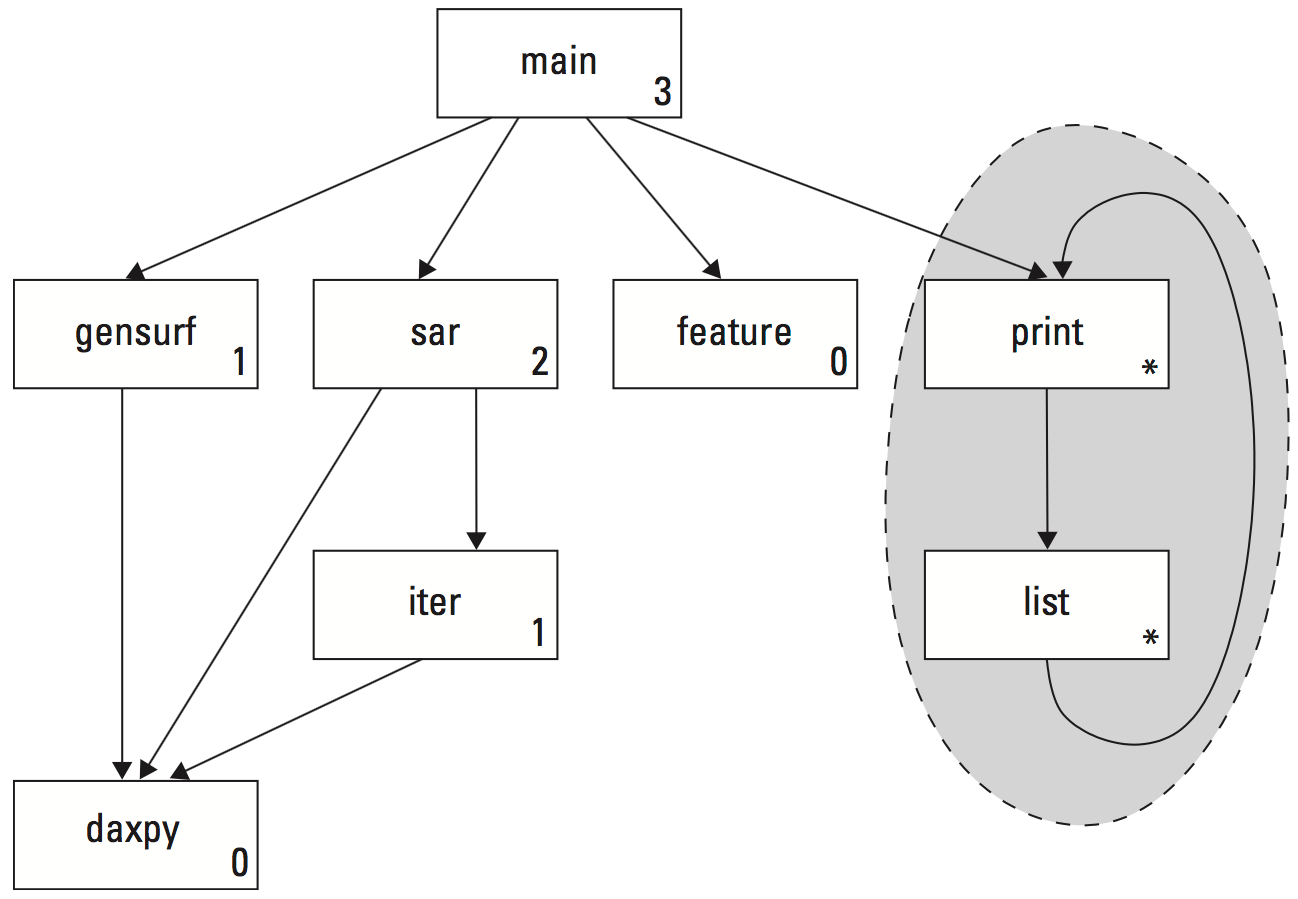
\includegraphics[width=0.6\textwidth]{img/f4-4.png}
				\caption{Análise de funções na qual os comandos \texttt{print} e \texttt{list} repetem inúmeras vezes.}
				\label{fig:perf_print_list}
			\end{figure}

			O exemplo da Figura \ref{fig:perf_print_list} mostra que as funções \texttt{print} e \texttt{list} formam um componente fortemente conectado e são marcados com um *. Em seguida, os vértices restantes de $ G $ são assinalados por uma regra ordinal,

			$$
			\text{ord}(u) =
			\left\{\begin{matrix}
			0 & \text{se nó } u \text{ é uma folha} \\
			\underset{(u,v) \in E(G)}{\max}\ \{ \text{ord}(v) \} + 1 & \text{caso contrário}
			\end{matrix}\right.
			$$


	\subsubsection{Modelo \textit{Multithread}}
		Além do modelo coprocessado, tem-se o modelo \textit{multithreads} que emerge como uma importante técnica de programação utilizada até em computadores com multiprocessadores. Neste modelo, o paralelismo natural do \hardware\ é conhecido e o \designer\ reconhece que o processador e os componentes executam continuamente. A coordenação desses componentes é manuseada por comunicações primitivas que tem sido desenvolvidas por processo concorrentes como semáforos, mensagens e outros. Cada \hardware\ é considerado um componente que executa como uma \textit{thread} paralela e o sistema de semáforos é utilizado para deixar o sistema consistente e assim, ao invés de bloqueado, o \hardware\ conceitualmente fica em bloqueio esperado pelo semáforo ou por uma mensagem.


	\subsubsection{Modelo de Rede em Chip}
		Este modelo investiga o estado distribuído completamente e depende da troca de mensagem para explicitar o estado. A coordenação é implícita com a transferência de estado. Como é assumido que o \design\ referencial de \software\ foi construído com comandos de troca de mensagem explícita, não se considera em um manual de sistemas embarcados. Entretanto, tem-se visto que técnicas de alta-performance continuam filtrando-se para o nível de sistemas embutidos.


\section{Programação Linear Inteira (PLI)} \label{sec:pli}
	Este problema representa um subgrupo da programação linear no qual algumas ou todas as variáveis do problema pertencem ao conjunto dos números inteiros. A tentativa de solucionar um PLI para um modelo puro com quantidades de restrições é um problema $\mathcal{NP}$-difícil.

	Um modelo de PLI pode ser obtido com a seguinte característica:

	\begin{equation}
			\begin{array}{rrcll}
			\text{min}  &  c' x    &  ~     &  ~            &  ~               \\
			subject\ to &  a'_i x  &  \leq  &  b_i,         &  \quad i \in M_1 \\
			~           &  a'_i x  &  \geq  &  b_i,         &  \quad i \in M_2 \\
			~           &  a'_i x  &   =    &  b_i,         &  \quad i \in M_3 \\
			~           &  x_j     &  \in   &  \mathbb{Z},  &  \quad j \in N_1 \\
			~           &  x_j     &  \in   &  \mathbb{Z},  &  \quad j \in N_1 \\
			\end{array}
            \label{eq:constraints_pli}
	\end{equation}
    
    onde:
    
    \begin{description}
    	\item [$c'x:$] é uma função linear de custo;
    	\item [$x:$] variáveis de decisão;
    	\item [$a':$] coeficientes fixos;
    	\item [$a'x \leq b, a'x = b$ e $a'x \geq b:$] restrições para validação da solução.
    \end{description}


\section{Questões} 

	\subsection{\textit{Profiling}} \label{sec:dificuldades}

			Uma suposição não adequada com a formulação analítica é que ela usa informação de \textit{profile} para aproximar o tempo de fração que uma aplicação gasta em uma sub-rotina ou bloco básico, mas no entanto, várias situações podem gerar resultados enganosos.



		\subsubsection{Execução Dependente de Dados}

			Quanto um simples conjunto de dados não representa o tempo gasto de cada sub-rotina quando este é alterado a sub-rotina não terá mudanças substanciais com a mudança do dado de entrada. A detecção da situação onde um único conjunto de dados não é representativo torna a situação difícil e requer que o \designer\ do sistema compreenda a operação fundamental da aplicação como é o caso da análise de complexidade das rotinas. É possível analisar esses casos com alguns métodos sendo a análise manual dos algoritmos e suas operações básicas, a coleta de informações \textit{profiling} baseado em diferentes conjuntos de dados ou mesmo a tentativa de separar a aplicação talvez ao longo dos limites do módulo e fazer o \textit{profile} de cada módulo independente.

		\subsubsection{Comportamento Correlacionado}

			Outra questão surge em aplicações que explicita o uso de eventos cronometrados. Muitos \textit{profile} assumem que a aplicação fará um progresso estável em direção à solução mas algumas aplicações incorporam o tempo. Sistemas de \textit{profiles} usam um temporizador de intervalo para amostrar o contador de programas dependendo da aplicação para não serem correlacionados estatisticamente com o temporizador. No entanto, se a aplicação possui operações executando em tempos regulares, periódicos, então os resultados do \textit{profiling} podem ser considerado enganosos. Por exemplo, se uma aplicação é executada a cada 10ms e a amostragem é feita a cada 10ms, então o \textit{profiler} não fornecerá dados concretos referentes ao sistema.



		\subsubsection{Comportamento Faseado}

			Sobre a totalidade de sua execução, o controle se move entre \textit{clusters} de operações relacionadas, isso é, a execução de uma aplicação exibida localmente. Como um exemplo, consideremos uma aplicação que possui três rotinas. Assumindo que cada possui $ 33\% $ de tempo de execução, e que cada tem a possibilidade de ter um \speedup\ de 50\% e postas de forma ordenada da primeira à última. Se existe espaço somente para uma rotina em recursos de FPGA, então o \speedup\ máximo será de 12\%. Mas se o comportamento faseado é suportado pelo \design\ de sistema, então há mais opções. Um é olhar procurar itens em comum sobre os três \textit{cores} e uma segunda é um \hardware\ multiplexado por tempo. Não há abordagens automáticas para esse.



		\subsubsection{Efeitos de I/O}

			\textit{Profiles} não contam tempo de I/O tais como acesso ao espaço de usuário e dispositivos realizando algum procedimento de busca ou ação.



		\subsubsection{Números de Chamada}

			\textit{Profiles} entretanto continuará a calcular quando sub-rotinas são invocadas. É importante ter noção o quanto uma sub-rotina é invocada.

	\subsection{Estrutura de Dados}

		Design de referência de \software\ naturalmente reflete um viés em relação às implementações em \software. Isso é compreensível, já que a programação é ensinada no contexto de modelo de computação sequencial ordinário. Com esses modelos, a diferença entre

	\begin{verbatim}
	while( i!=NULL ) {
	  proc(i) ;
	  i = i->next ;
	}
	\end{verbatim}
	e
	\begin{verbatim}
	while( i<n ) {
	 proc(x[i]) ;
	 i=i+1;
	}
	\end{verbatim}

		é insignificante já que ambos tomam $ \mathcal{O}(n) $ passos, mas em nível de \hardware\ o último pode ser mais desejável sendo no mínimo, uma ampla janela de pré-busca é possível. Se pudermos determinar que, em várias iterações do ciclo, cada \texttt{proc(x[i])} é independente, então pode-se melhorar o \design\ por meio de \textit{pipeline} ou paralelismo regular.

		O \design\ de referência de \software\ serve como extremamente bem como uma especificação, mas se executar um \textit{profile} do \design\ de referência, não será capturado os benefícios da implementação pois esses benefícios provem de alterações algorítmicas e são improváveis de serem reveladas por técnicas automáticas. Consequentemente, cai sobre o \designer\ de sistema compreender ambos o algoritmo de \software\ implementado no \design\ referencial e como pode ser re-implementado em \hardware.

		Há vários formas comuns de estruturas de \software\ que pode ser rearranjadas para produzir melhor \design\ de \hardware. Estruturas de dados que utilizam ponteiro como listas encadeadas, árvores, etc. podem ser representadas por uma estrutura ``\textit{flat}'' como vetores e arranjos produzindo acesso regular em memória que podem ser pré-buscadas subsequentemente ou utilizadas em \textit{pipeline}. Outra forma de ganho de performance é no tamanho de bit. Programadores de \software\ geralmente assumem um valor fixo, mesmo que utilizem somente poucos bits de informação. Enquanto \software\ tem caminho de dados fixos e relativamente baixa largura de banda entre componentes, \hardware\ se destaca no gerenciamento de largura de bits arbitrárias sendo possível alavancar grande largura de banda fornecida pela interconexão programável do FPGA.

	\subsection{Manipulando Tamanho de Recurso}

		A mudança mais simples envolve quebrar uma sub-rotina em sub-rotinas menores fazendo com que o recurso em \hardware\ fique menor e mais fácil de ser implementado.

		Há três momentos que agregar sub-rotinas são necessárias. Se duas sub-rotinas tomam 25\% cada uma do tempo da aplicação, então elas são candidatos fortes para a implementação em \hardware. No entanto, se for implementado individualmente, cada uma invoca o custo da sua interfaceação. Se há três sub-rotinas relacionadas (uma invocando a próxima), então a combinação delas pode reduzir o custo de invocações. Entretanto, o custo da interface não é sempre insignificante e vale a pena o esforço do usuário para investigar a situação.

		Qualquer outra mudança é substancial. Frequentemente, implementação em \hardware\ tem performance significativa por ter formato de dados de dados específicos da aplicação. Para que o \software\ seja mais eficiente nos formato de dados não padronizados, programadores irão investir em estruturas de dados que não são bem mapeadas para o \hardware. Assim, vale a pena olhar para o propósito e considerar a substituição de estruturas de dados para melhor explorar o \hardware.


\end{comment}


\begin{comment} %comment Módulos e Interfaces em \Design\ de \Software
\section{Conceitos e Componentes de \Design\ de Sistemas}
% \subsection{Módulos e Interfaces}
%Existem duas filosofias de \design\ para a construção de um sistema. Em um delas é possível realizar a especificação de cada função do projeto, chamado de blocos básicos\footnote{Um bloco básico é uma sequência maximal de instruções sequenciais com \textit{single entry and single exit} (SESE).}, e conectá-los logicamente de acordo a fim gerar o sistema completo. Tal é descrito como abordagem \textit{bottom-up}.
%A segunda baseia-se na descrição de um sistema completo e geral sendo que, em seguida, o \designer\ desmembra-o definindo seus sub-blocos até chegar ao nível mais básico de suas funções. Essa é chamada de abordagem \textit{top-down}.
%O conceito de abordagem de desenvolvimento de projetos é importante para descrever os conceitos de módulo e interface.%, segundo \citet{Sass2010}.

\subsection{Módulos e Interfaces em \Design\ de \Software}
\citet{Sass2010}, em seu livro, descreve que módulo é qualquer conjunto de operação auto-contidas que possui um nome, interface formal e geral e alguma descrição funcional. Isso significa que qualquer procedimento, mesmo que em \software\ ou em descrição de \hardware, que possa ser representado por uma caixa graficamente é considerado um módulo.
Define-se por interface formal o nome do módulo e a enumeração de duas operações, incluindo suas entradas e saídas, caso existam e a interface geral inclui todas as características da interface formal e qualquer protocolo ou comunicação adicional implícita. Com a interface formal descrita, é possível realizar inspeções mecânica e técnica no módulo enquanto a geral, o entendimento desse em alto nível.
Por último, um módulo pode ter também uma descrição funcional no qual pode ser implícita, formal ou informal. Quando a descrição é implícita, a descrição está presente de forma clara no nome do módulo, como por exemplo \texttt{full\_adder}. A formal consiste na documentação ou em meios matemáticos e comentários formais sobre as operações do módulo e a informal pode ser comentários descritivos ao longo da escrita da função.

Outros termos importantes são implementação e instância. Uma implementação é a realização de uma funcionalidade pretendida de um módulo mesmo que este tenha várias implementações como é permitido num ambiente de descrição de \hardware\ criar várias arquiteturas diferentes para um mesmo módulo.
Já a instância é o uso de uma implementação.
Enquanto em instâncias em nível de \software\ imagina-se relações um-a-um entre implementação e instância, em \hardware\ é comum o uso de copias físicas de cada implementação, sendo cada cópia representa uma instância no final. Na Figura \ref{fig:instance} é possível ver em \textit{a)} um instância padrão de uma implementação e em \textit{b)} uma outra instância com uma identificação única.

\begin{figure}[h] \centering
\includegraphics[width=0.7\textwidth]{img/f3-2.png}
\caption{Instâncias e suas descrições. Fonte: \cite{Sass2010}.}
\label{fig:instance}
\end{figure}

Como exemplificação, pode-se construir um somador completo de 4-bit utilizando várias instâncias da implementação do somador completo de 1-bit, exibido na Figura \ref{fig:somador_instancias}.

\begin{figure}[h] \centering
\includegraphics[width=0.98\textwidth]{img/f3-3.png}
\caption{Somador completo 4-bit utilizando instâncias de 1-bit. Fonte: \cite{Sass2010}.}
\label{fig:somador_instancias}
\end{figure}
\end{comment}

\begin{comment}
\subsection{Abstração e Estado}
\subsection{Coesão e Acoplamento}
\end{comment}




\begin{comment}
\section{Publicações}

	Neste apêndice são listados os trabalhos publicados em eventos científicos desenvolvidos durante o período de realização da presente pesquisa.

	\begin{enumerate}
		\item a
	\end{enumerate}

	O trabalho a seguir foi submetido e aceito para publicação em eventos científico.

	\begin{enumerate}
		\item  a
	\end{enumerate}
\end{comment}

\begin{comment}
\section{Reprodutibilidade}

	O código fonte do resolvedor desenvolvido no presente trabalho foi disponibilizado no seguinte endereço \todo{url.rar}. Convido o leitor interessado a validar os resultados obtidos bem como dar continuidade ao trabalho. A Tabela \ref{tab:parametros} apresenta uma lista de parâmetros que podem ser passados ao resolvedor via linha de comando.

	\begin{table}[H]
	\caption{Lista de parâmetros para o resolvedor}
	\begin{tabular*}{20cm}{lp{12cm}}
	-xml= & Arquivo de entrada para o resolvedor (obrigatório) \\
	-out= & Arquivo para o qual a solução obtida será salva (obrigatório) \\
	-time\_limit= & Limite de tempo de execução em segundos (obrigatório) \\
	-seed= & ``Semente'' aleatória (obrigatório) \\
	-alg= & Seleciona o algoritmo a ser aplicado (obrigatório) \\
	\\
	-bl\_max & Máximo de iterações do método de descida (Não Ascendente Randômico) \\
	\\
	-sa\_max & Máximo de iterações por temperatura no algoritmo SA \\
	-sa\_alpha & Razão de esfriamento do algoritmo SA \\
	-sa\_tempini & Temperatura inicial do algoritmo SA \\
	-sa\_tempmin & Temperatura mínima do algoritmo SA (usualmente 0)\\
	-sa\_reheats & Número de reaquecimentos do algoritmo SA\\
	\\
	-ils\_max & Máximo de iterações por temperatura no algoritmo SA \\
	-sa\_alpha & Razão de esfriamento do algoritmo SA \\
	-sa\_tempini & Temperatura inicial do algoritmo SA \\
	-sa\_tempmin & Temperatura mínima do algoritmo SA (usualmente 0)\\
	-sa\_reheats & Número de reaquecimentos do algoritmo SA\\


	\label{tab:parametros}
	\end{tabular*}
	\end{table}

\end{comment}

\end{appendices}
\let\cleardoublepage\clearpage
%% Produce the un-numbered back matter (e.g. colophon,
%% bibliography, tables of figures etc., index...)
\begin{backmatter}
	%!TEX root = ../Dissertacao.tex

\bibliographystyle{kluwer}
\bibliography{bibliography}
\printindex
\end{backmatter}

%% Close
\end{document}
